
%Aaron Titus
%PHY 2010 Lab Manual
%
%lab.cls file is from Benjamin Crowell, www.lightandmatter.com

\documentclass[10pt]{tituslab}
\usepackage{hyperref}
\usepackage{mandi131}
\usepackage{listings}
\usepackage{moreverb}
\usepackage{array}
\usepackage{pifont}
\usepackage{url}


% Typeset a block of code
% Use this as an alias for the lstlisting environment provided by listings package
\lstnewenvironment{myvpython}{\lstset{language=Python,numbers=none,upquote=true,breaklines,showstringspaces=false}}{}
\definecolor{vpythoncolor}{rgb}{0.95,0.95,0.95}
\lstset{backgroundcolor=\color{vpythoncolor}} 
\lstnewenvironment{vpythonprogram}{\lstset{language=Python,numbers=left,upquote=true,breaklines,showstringspaces=false}}{}
\lstnewenvironment{arduinoblock}{\lstset{language=C,numbers=left,numberstyle=\tiny,upquote=true,breaklines}}{}


%commands for frames
\newcommand{\tightframe}[1] {
	\ \\
	\noindent
	\fbox{
			\parbox[l]{5.5in}{
			#1 
		}
	}
}

\newcommand{\tinyanswerspace}{
\vspace{0.25in}
}
\newcommand{\smallanswerspace}{
\vspace{0.5in}
}

\newcommand{\tinyframe}[1] {
	\ \\
	\noindent
	\fbox{
			\parbox[l]{5.5in}{
			#1 
			\vspace{0.5in}
		}
	}
}

\newcommand{\smallframe}[1] {
	\ \\
	\noindent
	\fbox{
			\parbox[l]{5.5in}{
			#1 
			\vspace{1in}
		}
	}
}

\newcommand{\medframe}[1] {
	\ \\
	\noindent
	\fbox{
			\parbox[l]{5.5in}{
			#1 
			\vspace{2in}
		}
	}
}

\newcommand{\bigframe}[1] {
	\ \\
	\noindent
	\fbox{
			\parbox[l]{5.5in}{
			#1 
			\vspace{4in}
		}
	}
}

%%%%%%%%%%%%%%%%%%%%%%%%%%%%%
% commands for images
%an image with caption
\newcommand{\image}[2]{
\begin{figure}[h!]
\begin{center}
\includegraphics[scale=1]{#1}
\caption{#2}
\label{#1}
\end{center}
\end{figure}
}

%an image with caption and scale
\newcommand{\scaledimage}[3]{
\begin{figure}[h!]
\begin{center}
\includegraphics[scale=#3]{#1}
\caption{#2}
\label{#1}
\end{center}
\end{figure}
}
%%%%%%%%%%%%%%%%%%%%%%%%%%%%%
%commands for menu names, filenames, hyperlinks,  ...
%scientific notation with no units
\newcommand{\menu}[1]{
	{\bf #1}
}
\newcommand{\link}[1]{
	\texttt{#1}
}
\newcommand{\file}[1]{
	\emph{#1}
}
\newcommand{\button}[1]{
	\fbox{#1}
}

%%%%%%%%%%%%%%%%%%%%%%%%%%%%%
%units and constants

%units and common expressions
\newcommand{\kg}{\ensuremath{\kilogram}}
\newcommand{\m}{\ensuremath{\meter}}
\newcommand{\km}{\ensuremath{\kilo\meter}}
\newcommand{\mps}{\ensuremath{\meter\per\second}}
\newcommand{\mpss}{\ensuremath{\meter\per\second \squared}}
\newcommand{\kgmps}{\ensuremath{\kilogram \usk \meter\per\second}}
\newcommand{\angmom}{\ensuremath{\kilogram \usk \meter \squared \per\second}}
\newcommand{\rps}{\ensuremath{\radian \per\second}}
\newcommand{\npkg}{\ensuremath{\newton \per \kilogram}}
\newcommand{\N}{\ensuremath{\newton}}
\newcommand{\n}{\ensuremath{\newton}}
\newcommand{\gearth}{\ensuremath{\unit{9.8}{\npkg}}}
\newcommand{\gpm}{\ensuremath{\gram \per \mole}}



%%%%%%%%%%%%%%%%%%%%%%%%%%%%%
%math formatting

%adds parenthesis, especially useful for numerical constants
\newcommand{\lr}[1]{\ensuremath{\left(#1\right)}} %adds \left and \right parenthesis around quantity

%a vector with no units
\newcommand{\triple}[3]{
	\ensuremath{\langle #1, #2 , #3 \rangle}
}

%scientific notation with no units
\newcommand{\sci}[2]{
	\ensuremath{#1 \times 10^{#2}}
}
\newcommand{\scie}[2]{
	\ensuremath{#1 \mbox{e} {#2}}
}
\newcommand{\sciE}[2]{
	\ensuremath{#1 \mbox{E} {#2}}
}

%zero vector with units
\newcommand{\vectzero}[1]{\ensuremath{\vectncomps{0}{0}{0}{#1}}}
%zero vector with no units
\newcommand{\zerovect}{\ensuremath{\triple{0}{0}{0}}}
%zero vector with units
\newcommand{\zerovectunits}[1]{\ensuremath{\vectncomps{0}{0}{0}{#1}}}

%common math equations; the entire equation with & = &
%unit vector
\newcommand{\equnitvectsub}[2]{\ensuremath{\vectsubhat{#1}{#2} & = & \frac{\vectsub{#1}{#2}}{\vectsubmag{#1}{#2}}}}
%momentum principle delta p = Fnet delta t
\newcommand{\eqmpDp}{\ensuremath{\Delta \vec{p} & = & \vectsub{F}{net}\Delta t}}
%momentum principle delta p = Fnet delta t
\newcommand{\eqmpupdate}{\ensuremath{ \pfin & = & \pinit + \vectsub{F}{net}\Delta t}}
%traditional f=ma
\newcommand{\eqmpma}{\ensuremath{\vectsub{F}{net} & = & \frac{\Delta \vec{p}}{\Delta t}\\
& = & m\frac{\Delta \vectsub{v}{cm}}{\Delta t}\\
& = & m \vectsub{a}{cm}\\
}}

%pf
\newcommand{\pfin}{\ensuremath{\vectsub{p}{f}}}
%pi
\newcommand{\pinit}{\ensuremath{\vectsub{p}{i}}}

%unit vector with subscript
\newcommand{\hatsub}[2]{\ensuremath{\vectsubhat{#1}{#2}}}

%%%%%%%%%%%%%%%%%%%%%%%%%%%%%%%%%
%computer code
\newcommand{\type}[1]{
	{\texttt{#1}}
}
\newcommand{\code}[1]{
	{\texttt{#1}}
}

\newcommand{\report}{
	\newpage 
	\section*{Lab Report}
}


\begin{document}
\myeqnspacing % Do this early and often, since it gets reset by \normalsize
%========================= frontmatter =========================
\frontmatter
\yesiwantarabic
\frontmatter
\thispagestyle{empty}
\noindent\vspace{0mm}\\
\noindent\vspace{10mm}\hspace{1mm}\textsf{\textbf{\LARGE{PHY 1200: Physics for Video Games (with GlowScript)}}}\\
\noindent\vspace{4mm}\hspace{4in}\textsf{\Large{Notes, Labs, and Programs}}\\
\noindent\vspace{4mm}\hspace{4in}\textsf{\Large{Aaron Titus}}\\
\noindent\vspace{4mm}\hspace{4in}\textsf{\Large{High Point University}}\\
\noindent\vspace{4mm}\hspace{4in}\textsf{Spring 2016}\\
\noindent\vspace{4mm}\hspace{4in}\textsf{http://physics.highpoint.edu/$\sim$atitus/}
\yesiwantarabic
\mynormaltype

\pagebreak[4]
\noindent
Copyright (c) 2011 by A. Titus. This lab manual is
    licensed under the Creative Commons
    Attribution-ShareAlike license, version 1.0, 
    http://creativecommons.org/licenses/by-sa/1.0/.
    If you agree to the license, it grants you certain privileges that
    you would not otherwise have, such as the right to copy the book,
    or download the digital version free of charge from
    \href{http://physics.highpoint.edu/~atitus/}{http://physics.highpoint.edu/$\sim$atitus/}. At your option, you may also copy this book
    under the GNU Free Documentation License version 1.2, http://www.gnu.org/licenses/fdl.txt,
    with no invariant sections, no front-cover texts, and no back-cover texts.


\tableofcontents
%========================= main matter =========================
\mainmatter
\startchaptersonleftpage
%-- I want the whole book numbered sequentially, arabic:
\pagenumbering{arabic} 
\addtocounter{page}{4} 
\parafmt
\myeqnspacing % Do this early and often, since it gets reset by \normalsize
%\twocolumn

\lab{Coordinates}

\section*{Cartesian Coordinate System}

To specify the location of an object, we use a coordinate system. The one shown in Figure \ref{coordinates/2d-coordsystem} is a two-dimensional (2-D) Cartesian coordinate system with the $+x$ direction defined to the right and the $+y$ direction defined to be upward, toward the top of the page.

\scaledimage{coordinates/2d-coordsystem}{A 2-D Cartesian coordinate system.}{0.5}

A three-dimensional (3-D) coordinate system with the $+z$ axis defined to be outward toward you, perpendicular to the page, is shown in Figure \ref{coordinates/3d-coordsystem}.

\scaledimage{coordinates/3d-coordsystem}{A 3-D Cartesian coordinate system.}{0.5}

A coordinate system is defined by:

\begin{enumerate}
	\item an origin
	\item a scale (determined by the tick marks, numbers, and units)
	\item an orientation; the direction of the +x, +y, and +z directions, respectively. 
\end{enumerate}

The orientation is described verbally by saying something like ``The +x direction is toward the right of the origin.'' Or, ``The +y direction is upward toward the top of the page.''

\section*{Coordinates}

A point on a Cartesian coordinate system is designated by a pair of numbers in 2-D and a triplet of numbers in 3-D. On a 2-D coordinate system, the pair of numbers represents the $(x,y)$ coordinates of the point.

On the coordinate system in Figure \ref{coordinates/x-y-points}, the red dot is at the location $(+1,+3)$ meters. And the blue dot is at the location $(+4,-4)$ meters. Thus, we say that the x-position of the red dot is $+1$ m, and the y-position of the red dot is +3 m. Likewise, the x-position of the blue dot is +4 m, and the y-position of the blue dot is -4 m.

\scaledimage{coordinates/x-y-points}{Coordinates of certain points on a coordinate system.}{0.5}

The sign of the coordinate tells us the side of the origin that the point is on. Thus, $x=+1$ means that the point is on the right-side of the origin. If $x=-1$ then the point is on the left-side of the origin.

Likewise, $y=+3$ means that the point is above the origin, and $y=-4$ means that the point is below the origin.

\tightframe{
{\bf Question:}  State in words the location of a point with a positive z-coordinate.

{\bf Answer:}  Using the coordinate system in Figure 1.2, a positive value of z means that the point is in front of the page (which we assume to be the x-y plane), toward you. For example if you are reading this page, then your eyes have positive z coordinates.
}

\section*{Computer Convention}

Programming languages define the origin of the monitor to be at the top left corner. The $+x$ axis is to the right, and the $+y$ axis is downward, as shown in Figure \ref{coordinates/comp-coords}. 

The units, in computer graphics, are pixels. If the resolution of a monitor is is $1440 \times 900$, it means that the monitor displays 1440 pixels horizontally and 900 pixels vertically. Since the origin is in the top left corner, the coordinates of a single pixel on a monitor are always positive.

\scaledimage{coordinates/comp-coords}{Convention for pixel coordinates on a computer monitor.}{0.5}

\section*{Example}

\tightframe{
{\bf Question:}  What are the coordinates of point A in Figure \ref{coordinates/points}?

{\bf Answer:}  For point A, $x=+2\ \meter$ and $y=+3\ \meter$. Thus, it's coordinates are $(+2, +3)\ \meter$.
}

\scaledimage{coordinates/points}{Three points on a Cartesian coordinate system.}{0.4}

\pagebreak

\section*{Homework}

\begin{enumerate}
	\item What are the coordinates of points B and C in Figure \ref{coordinates/points}?
	\item A puck travels across the monitor in a computer game as shown in Figure \ref{coordinates/puck}. The top left corner of the image is the origin. Each line on the grid represents 10 pixels. The puck moves from the top, right side of the monitor to the bottom, left side of the monitor. What are the coordinates in pixels of each image of the puck?

\scaledimage{coordinates/puck}{A puck on a computer monitor.}{1}
	
\end{enumerate}
\lab{LAB:  Coordinates}

\apparatus
\equip{meterstick or tape measure}
\equip{graph paper}

\longgoal

To measure the coordinates of objects in the classroom.

\procedure

\begin{enumerate}
	\item Define the origin of our coordinate system to be at the left corner of the front of the room (if you are facing toward the front), at the floor.
	\item Define the $+x$ direction to be to the right, if facing the front of the room.
	\item Define the $+y$ direction to be upward toward the ceiling.
	\item Define the $+z$ direction to be along the side wall toward the back of the room.
	\item Using a meterstick, determine the coordinates of the center of the seat of your chair.
\end{enumerate}

\extension

\begin{description}
	\item [C] What are the coordinates of the center of your seat?
	\item [B] (Do C first.) Using graph paper, draw an x-z coordinate system with the origin in the top-left corner of the paper. (Note: it's ok to use your paper in landscape or portrait orientation depending on what is most convenient. You are sketching a top view of the room. Assume that the front wall with the whiteboard is at the top edge of the paper.) Draw the seat of your chair (as a circle) at the correct location on the coordinate system. Assume that the chair is underneath the table. Be sure to indicate the scale of your coordinate system by labeling the axes with both numbers and units. Sketch the boundaries of the room. Select the values of your gridlines so that the coordinate system takes up as much of the paper as possible.
	\item [A]  (Do B and C first.) Determine the coordinates of the center of your table in the room. Measure the length and width of the table and accurately sketch the boundary of your table on the coordinate system.
\end{description}

\lab{PROGRAM:  Introduction to GlowScript and VPython}

\apparatus
\equip{Computer}
\equip{GlowScript -- www.glowscript.org}

\longgoal

The purpose of this activity is to write your first program in a language called Python. We will use the web app GlowScript that converts Python to JavaScript so the program can run in a web browser. GlowScript provides the same functions available in the Python module called Visual. Together Python and Visual are named VPython. As a result, GlowScript can be considered the web-based version of VPython. You will probably read or hear the terms GlowScript and VPython used interchangeably; however, there are some important differences. I tend to think of the language as VPython (Python + Visual) and the web app as GlowScript.

We use VPython because it allows you to do vector algebra and to create 3D objects in a 3D scene. The capability of 3D graphics with vector mathematics makes it a great tool for simulating physics phenomena. In this activity, you will learn:

\begin{itemize}
	\item how to use GlowScript, the web-based integrated development editor (IDE) for writing and running VPython.
	\item how to structure a simple computer program in VPython.
	\item how to create 3D objects such as spheres and arrows.
%	\item how to define vectors in VPython.
%	\item how to add and subtract vectors in VPython.
\end{itemize}

\setup

Go to \href{http://www.glowscript.org/}{http://www.glowscript.org/} and create an account. You will need a Google account because GlowScript uses your Google account for authentication. After logging in, you will see a link to ``your programs are here.'' Click this link to enter the IDE. 

\procedure

\begin{enumerate}

	\subsection*{Creating folders and files}
	
	\item Once you log in and follow the link to your programs, you are in the GlowScript IDE. Click the 
\includegraphics[scale=0.75]{glowscript-intro/gs-add-folder} tab to create a new folder. A pop-up window appears as shown in Figure \ref{glowscript-intro/gs-new-folder}. Because I must run your programs, make the folder public. Name it ``phy1200'' if you wish.
	
	%{\bf \emph{Uncheck}} Public in order to make the folder PRIVATE. This is important so others cannot see your work as you are developing. After you create games for your projects, you will copy them to a public folder to share them with the world. Name the folder ``phy1200private'' or whatever you wish. Later you will probably make a ``phy1200public'' folder.
	
	\scaledimage{glowscript-intro/gs-new-folder}{Create a new folder in GlowScript.}{0.5}


	\item With the folder name highlighted orange (showing you are in the folder), click the link {\bf Create New Program} and name the program \code{intro}.
	
		
	\subsection*{Starting a program:  Setup statements}
	
	\item Notice GlowScript types the first line of the program for you.
	
\begin{myvpython}
GlowScript 1.1 VPython
\end{myvpython}
	
Every GlowScript program begins with this setup statement. It tells GlowScript you are writing VPython code.

	\item Also, notice there is no ``save'' menu. Like Google Docs, GlowScript automatically saves your program as you are typing it. 
	
	\subsection*{Creating an object}

	\item Now for your first VPython command, let's make a sphere. Skip a line in order to make your code more readable, and on line 3, type:

\begin{myvpython}
sphere()
\end{myvpython}

This statement tells the computer to create a sphere object.

	\item Run the program by clicking {\bf Run this program}. GlowScript exits the edit mode and enters the run mode. You should see a white sphere on a black background like Figure \ref{glowscript-intro/sphere}. This is called the \code{scene}.

	\scaledimage{glowscript-intro/sphere}{Your first VPython program--a sphere.}{0.5}


	\subsection*{The 3-D graphics scene}
	
By default the sphere is at the center of the scene, and the ``camera'' (your point of view) is looking directly at the center.
	
	\item If you are on a PC, hold down both mouse buttons and move the mouse forward and backward to make the camera move closer or farther away from the center of the scene. On a Mac, hold down the option key while moving the mouse forward and backward. This is how you \emph{zoom} in VPython.
	
	\item Hold down the right mouse button alone and move the mouse to make the camera ``revolve'' around the scene, while always looking at the center. On a Mac, in order to rotate the view, hold down the Control key while you click and drag the mouse. This is how you \emph{rotate} the scene in VPython. Because this is a sphere, you won't notice a significant change except for lighting.

By default, when you first run the program, the coordinate system is defined with the positive x direction to the right, the positive y direction pointing up toward the top edge of the monitor, and the positive z direction coming out of the screen toward you. You can then rotate the camera view to make these axes point in other directions relative to the camera. 
		
	\subsection*{Error messages: Making and fixing an error}
	
	GlowScript tells you when there is a syntax error in  your program. (Logic errors are much more difficult to fix!) To see an example of an error message, let's try making a spelling mistake.
	
	\item Click {\bf Edit} to return to editing mode, and change line 3 of the program to the following:
	
\begin{myvpython}
phere()
\end{myvpython}

	\item Run the program.

There is no function or object in VPython called phere(). As a result, an error message pops up. The message gives the \emph{approximate} line number where the error occurred and a description of the error, as shown in Figure \ref{glowscript-intro/gs-error}.

	\scaledimage{glowscript-intro/gs-error}{An error message in GlowScript.}{0.5}

The line number may be off, as it is in this case but is usually close.

	\item Correct the error in the program by clicking {\bf Edit this program} and returning to the editor. Once in editing mode, you can click the \frame{X} to close the error message.

There are two types of errors: (1) syntax errors which might be a typing or coding mistake and (2) programmatic errors so the program runs correctly but does something other than what you intended. The error message helps you find the first of these. Finding errors that cause a program to act differently than you intended is much more difficult and is a skill you will develop in this course.
	
	\subsection*{Changing attributes (position, size, color, shape, etc.) of an object}
	
Now let's give the sphere a different position in space and a radius. 

	\item Change line 3 of the program to the following:

\begin{myvpython}	
sphere(pos=vector(-5,2,3), radius=0.40, color=color.red)
\end{myvpython}

	\item Run the program.  Experiment with other changes to pos, radius, and color, running the program each time you change an attribute.
	
	\item Answer the following questions:
	
	\tightframe{
What does changing the \code{pos} attribute of a sphere do?\\
\vspace{0.25in}

What does changing the \code{radius} attribute of a sphere do?\\
\vspace{0.25in}

What does changing the \code{color} attribute of a sphere do? What colors can you use?  You can try \code{color=vector(1,0.5,0)} for example. The numbers stand for RGB (Red, Green, Blue) and can have values between 0 and 1. Can you make a purple sphere? Note that colors such as cyan, yellow, and magenta are defined, but not all possible colors are defined. Choose random numbers between 0 and 1 for the (Red, Green, Blue) and see what you get. \\
\vspace{0.25in}

}

	\subsection*{Autoscaling and units}

VPython automatically zooms the camera in or out so all objects appear in the window. Because of this autoscaling, the numbers for the \code{pos} and \code{radius} can be in any consistent set of units, like meters, centimeters, inches, etc. For example, this could represent a sphere with a radius 0.20 m at the position $(2,4,0)$ m. In this course we will often use SI units in our programs (``Systeme International'', the system of units based on meters, kilograms, and seconds).

	\subsection*{Creating a box object}

Another object we will often create is a box. A box is defined by its position, axis, length, width, and height as shown in Figure \ref{glowscript-intro/box}.

\scaledimage{glowscript-intro/box}{Attributes of a box. (Image from  \url{http://www.glowscript.org/docs/VPythonDocs/box.html})}{0.7}

	\item Type the following on a new line, then run the program:

\begin{myvpython}
box(pos=vector(0,0,0), size=vector(2,1,0.5), color=color.orange)
\end{myvpython}

The length, width, and height of the box are expressed as a vector with the attribute:\\
  \code{size=vector(L,H,W)}.  

	\item Change the length to 4 and rerun the program.
	
	\item Now change its height and rerun the program.
	
	\item Similarly change its width and position.

\tightframe{
Which dimension (length, width, or height) should be changed to make a box longer along the y-axis? Change your code now to check your answer.\\
\vspace{0.25in}

What point does the position of the box refer to?
\begin{enumerate}
\item the center of the box
\item one of its corners
\item the center of one of its faces
\item some other point

\end{enumerate}
}

	\subsection*{Comment lines (lines ignored by the computer)}

Comment lines start with a \# (pound sign). 
A comment line can be a note to yourself, such as:

\begin{myvpython}
# units are meters
\end{myvpython}

Or a comment can be used to remove a line of code temporarily, without erasing it.

	\item Put a \# at the beginning of the line creating the box, as shown below.

\begin{myvpython}
#box(pos=vector(0,0,0), size=vector(2,1,0.5), color=color.orange)
\end{myvpython}

	\item Run the program. What did you observe?
	
	\item Uncomment this line by deleting the \# and run the program again. The box now appears.
	
	\subsection*{Naming objects; Using object names and attributes}
	
We will draw a tennis court and will change the position of a tennis ball.

	\item Clean up your program so it contains only the following objects:  

A green box that represents a tennis court. Make it 78 ft long, 36 ft wide, and 4 ft tall. Place its center at the origin.

An orange sphere (representing a tennis ball) at location \triple{-28}{5}{8} ft, with radius 1 ft. Of course a tennis ball is much smaller than this in real life, but we have to make it big enough to see it clearly in the scene. Sometimes we use unphysical sizes just to make the scene pretty.

(Remember, you don't type the units into your program. But rather, you should use a consistent set of units and know what they are.)

	\item Run your program and verify that it looks as expected. Use your mouse to rotate the scene so you can see the ball relative to the court. Your program should look like the one below.
	
\begin{vpythonprogram}
GlowScript 1.1 VPython

box(pos=vector(0,0,0), size=vector(78,4,36), color=color.green)

sphere(pos=vector(-28, 5, 8), radius=1, color=color.orange)

\end{vpythonprogram}
	
	
	\item Change the position of the tennis ball to \triple{0}{6}{0} ft. 

	\item Run the program.

	\item Sometimes we want to change the position of the ball after we defined it. Thus, give a name to the sphere by changing the \code{sphere} statement in the program to the following:

\begin{myvpython}
tennisball=sphere(pos=vector(0, 6, 0), radius=1, color=color.orange)
\end{myvpython}

We've now given a name to the sphere. We can use this name later in the program to refer to the sphere. Furthermore, we can specifically refer to the attributes of the sphere by writing, for example, \code{tennisball.pos} to refer to the tennis ball's position attribute, or \code{tennisball.color} to refer to the tennis ball's color attribute. To see how this works, do the following exercise.

	\item Start a new line at the end of your program (perhaps line 7) and type:

\begin{myvpython}
print(tennisball.pos)
\end{myvpython}


	\item Run the program.

	\item Look at the text below the 3D scene. The printed vector should be the same as the tennis ball's position.

	\item Add a new line to the end of your program (perhaps line 9) and type:
	
\begin{myvpython}
tennisball.pos=vector(32,7,-12)
\end{myvpython}
	
	When running the program, the ball is first drawn at the original position but is then drawn at the last position. (Note: whenever you set the position of the tennis ball to a new value in your program, the tennis ball will be drawn at that position.) This may happen so quickly that you do not notice the tennis ball drawn at the two locations.
	
	\item Add a new line to the end of your program (perhaps line 11) and type:
	
\begin{myvpython}
print(tennisball.pos)
\end{myvpython}

(Or just copy and paste your previous print statement.)

	\item Run your program. It now draws the ball, prints its position, redraws the ball at a new position, and prints its position again. As a result, you should see the following two lines printed:
	
\begin{verbatim}
<0, 6, 0>
<32, 7, -12>
\end{verbatim}
	
	Of course, this happens faster than your eye can see it which is why printing the values is so useful.

\end{enumerate}

\analysis

All games with graphics include objects on the screen. The game programmer must specify the positions and dimensions (sizes) of the objects using 2D or 3D vectors.

\begin{description}

\item[C] Do all of the following.
You are going to create objects for the game \emph{Frogger}. We will only use spheres and boxes for this part.
\begin{enumerate}
	\item Click the link to your username to return to your folders.
	\item If necessary, click the phy1200 folder. Create a new blank file and name it \emph{frogger-C}. 
	\item Create a green box for the frog that is at the location $<0,-100,0>$, has a length=10, height=10, and width=10 units. Name the box \code{frog}.
	\item Create a yellow sphere for a lily pad at $<-60,100,0>$ with a radius of 10. Name the sphere \code{lilypad}.
	\item Create a blue box for the water that is at the location $<0,0,-10>$, has a length=150, height=220, and width=10 units. Name the box \code{water}.
	\item Rotate the scene. Is the lily pad inside the water or on top of the water?  Is the frog inside the water or on top of the water?
	\item Is physics used in this program? Why does the frog not move in this program?
\end{enumerate}

\item[B] Do everything for {\bf C} along with the following modifications and additions.

\begin{enumerate}
	\item Return to your phy1200 folder and create a new blank file and name it \emph{frogger-B}. 
	\item Copy from your previous program (labeled C) and paste it into this program. Often, this is the fastest way to start a new program.
	\item Create another yellow sphere for a lily pad at $<60,100,0>$ with a radius of 10. Name the sphere \code{lilypad4}.
	\item In between these two lily pads, create two more named  \code{lilypad2} and  \code{lilypad3} so the lily pads are equally spaced.
	\item Create a gray road that is exactly half the height of the water. It should extend from the middle of the blue box to the bottom end of the blue box.
	\item Create a long cyan box on the left side of the road and a short magenta box on the right side of the road, between the frog and the water. Name them \code{car1} and \code{car2}.
	\item Print the positions of the cars and the frog.
\end{enumerate}

Figure \ref{glowscript-intro/gs-frogger-B} is an example program that fits the criteria for a B.

	\scaledimage{glowscript-intro/gs-frogger-B}{The scene required for a B.}{0.5}


\item[A] Do everything for {\bf B} along with the following modifications and additions.

\begin{enumerate}
	\item Return to your phy1200 folder and csreate a new blank file and name it \emph{frogger-A}. 
	\item Copy from your previous program (labeled B) and paste it into this program.
	\item In the top right corner of the GlowScript window, click the link to {\bf Help}. This opens the documentation window. Click the menu to {\bf Choose a 3D object} and view the list of objects shown in Figure \ref{glowscript-intro/gs-frogger-B}.

	\scaledimage{glowscript-intro/gs-help}{GlowScript documentation}{0.5}

	\item Select the cylinder and read how to create a cylinder.
	
	\item Change the lily pads so they are thin cylinders that appear to float on top of the water.
	
	\item Use the cylinder object to create 3 logs of different lengths in the water.
	
	\item Now, click the menu to {\bf Work with 3D objects} in the documentation and select {\bf Materials/Textures}. Read how to specify a texture. You will probably want to click the link to the example program that demonstrates the pre-defined textures.
	
	\item Change the three wooden logs so they use the wood texture.

\end{enumerate}

Figure \ref{glowscript-intro/gs-frogger-A} is an example program that fits the criteria for program A.

	\scaledimage{glowscript-intro/gs-frogger-A}{The scene required for an A.}{0.5}




\end{description}


\lab{Vectors}

\section*{Definition of a Vector}

To put it simply, a vector is an arrow. The arrow has a tail and a head, each of which is at a point on a coordinate system. Thus, the arrow can be defined by the coordinates of its head and the coordinates of its tail. In Figure \ref{vectors/vector}, the head of the vector is at $(+1,+4)\ \meter$, and the tail is at $(-4,-2)\ \meter$.

\scaledimage{vectors/vector}{A vector is simply an arrow.}{0.5}


\section*{Vector Components}

You can define a vector another way -- by specifying the coordinates of the tail and then specifying how many units over and upward (or downward) you have to count in order to get to the head of the vector. 

For example, in Figure \ref{vectors/vector-components}, the tail of the vector is at $(-4,-2)\ \meter$. To get to the head of the arrow, you can ``walk'' to the right 5 meters and then ``walk'' upward 6 meters. (By ``walking,'' I mean take your pencil and count over to the right along the dashed line until you get to the $+1$ coordinate. Then, count upward along the dotted line until you get to the head of the arrow.)

\scaledimage{vectors/vector-components}{The x and y components of a vector.}{0.5}

The dashed line, the dotted line, and the arrow form a right-triangle. The horizontal dashed line is parallel to the x-axis and is called the \emph{x-component} of the vector. The vertical dotted line is parallel to the y-axis and is called the \emph{y-component} of the vector. 

In the example in Figure \ref{vectors/vector-components}, the x-component of the vector is $+5$ meters, and the y-component of the vector is $+6$ vectors. We will write a vector's components using parentheses as well, such as $(+5,+6)\ \meter$. But note that coordinates $(x,y)$ are different than vector components (horizontal component, vertical component). They have different meanings.

The $+$ sign on the x-component means that we had to count over \emph{to the right}. The $+$ sign on the y-component means that we had to counter \emph{upward}. If we had counted to the left, then the x-component would be negative. If we had counted downward, then the y-component would be negative. 

Symbols for a vector are written with an arrow on top of them. For example, we could name this vector $\vect{A}$. Then, $\vect{A}=(+5,+6)\ \meter$. The x and y components are written as $A_x$ and $A_y$, respectively. So, in general  $\vect{A}=(A_x,A_y)$.

We can define the vector by the coordinates of its tail and its head. Alternatively, we can define the vector by the coordinates of its tail and the vector's components. These methods are identical and lead one to draw the same arrow. (See the summary in Table \ref{vectors/definition}.)

\begin{table}[htdp]
\caption{Two ways to define vector $\vec{A}$ in this example.}
\begin{center}
\begin{tabular}{|m{3in}|m{3in}|}

\hline
\hline
\begin{center}{\bf Method 1 to describe vector $\vect{A}$ }\end{center}  & \begin{center}{\bf Method 2 to describe vector $\vect{A}$ }\end{center} \\
tail location is at: $(-4,-2)\ \meter$ &  tail location is at: $(-4,-2)\ \meter$ \\
head location is at: $(+1,+4)\ \meter$ & vector components are: $(+5,+6)\ \meter$ \\
\hline
\hline
\end{tabular}
\end{center}
\label{vectors/definition}
\end{table}%


\section*{Head = Tail + Vector Components}

If you know the tail of a vector and you know its components, then you can calculate the coordinates of the head of the vector.

\begin{eqnarray*}
	\mbox{(head)}& = & \mbox{(tail)} + \mbox{(vector components)} \\
	\mbox{for example: } (+1,+4)\ \meter & = & (-4,-2) \ \meter + (+5,+6)\ \meter 
\end{eqnarray*}

To add the tail and vector components, you add the x-values and y-values separately. Thus,

\begin{eqnarray*}
	\mbox{x: }\qquad +1 & = & -4 +5 \\
	\mbox{y: }\qquad +4 &=& -2 + 6
\end{eqnarray*}

which gives the location of the head as:  $(+1,+4)\ \meter$. Maybe it is easier to write it vertically, as shown below.

\begin{eqnarray*}
	&  & (-4,-2) \ \meter \\
	& + & (+5,+6) \ \meter \\
	&  &\overline{ (+1,+4)\ \meter} 
\end{eqnarray*}

\section*{Vector Components = Head - Tail}

If you know the coordinates of the head and tail of a vector, you can calculate the vector's components by:

\begin{eqnarray*}
	\mbox{(vector components)}& = & \mbox{(head)} - \mbox{(tail)}\\
	\mbox{for example: }  (+5,+6)\ \meter & = &  (+1,+4)\ \meter - (-4,-2) \ \meter 
\end{eqnarray*}

Writing it vertically looks like:

\begin{eqnarray*}
	&  & (+1,+4) \ \meter \\
	& - & (-4,-2) \ \meter \\
	&  &\overline{ (+5,+6)\ \meter} 
\end{eqnarray*}

\subsection*{Examples}

\tightframe{

{\bf Question:}

The tail of vector is at (+3,-4) m. Its head is at (+1,-1) m. Does the vector point to the right or to the left?  Does the vector point upward or downward? \\

{\bf Answer:}

Find the vector components. 

\begin{eqnarray*}
	\mbox{(vector components)}& = & \mbox{(head)} - \mbox{(tail)}\\
	 & = &  (+1,-1)\ \meter -  (+3,-4) \ \meter \\
	 & = &  (-2,+3) \ \meter 
\end{eqnarray*}

Because the vector's x-component is negative, the vector points to the left. Because its y-component is positive, the vector points upward. You can also answer this question by drawing the vector on a coordinate system and observing that it points to the left and upward.

}

\bigskip

\tightframe{

{\bf Question:}

Computers, by default, define the $+x$ axis to the right and the $+y$ axis downward, with the origin at the top left corner of the monitor. The tail of vector $\vect{B}$ is at (300,100) pixels, and $\vect{B}=(150,200)$ pixels. Where is the head of $\vect{B}$? \\

{\bf Answer:}

\begin{eqnarray*}
	\mbox{(head)}& = & \mbox{(tail)} + \mbox{(vector components)} \\
	& = & (300,100)\ \mathrm{pixels} + (150,200)\ \mathrm{pixels} \\
	& = & (450,300)\ \mathrm{pixels} 
\end{eqnarray*}

}

\section*{Magnitude of a Vector}

Vectors have two essential properties:  (1) length and (2) direction. The length of a vector is also called its \emph{magnitude} and is written $|\vect{A}|$. 

The vector and its components make up a right triangle, as shown in Figure \ref{vectors/vector-components}. The vector is the hypotenuse, and the components are the sides.

Pythagorean's theorem for a right triangle is $c^2  =  a^2 + b^2$. When applied to a right triangle, Pythagorean theorem gives:

\begin{eqnarray*}
	|\vect{A}|^2 & = & A_x^2 + A_y^2 \\
\end{eqnarray*}

\subsection*{Example}

\tightframe{

{\bf Question:}

What is the length (i.e. magnitude) of $\vect{A}$ in Figure \ref{vectors/vector-components}? \\

{\bf Answer:}

$\vect{A}= (+5,+6)\ \meter$, so $|\vect{A}|$ is

\begin{eqnarray*}
	|\vect{A}| & = & \sqrt{A_x^2 + A_y^2} \\
	& = & \sqrt{(5\ \meter)^2 + (6\ \meter)^2} \\
	& = & 7.81\ \meter
\end{eqnarray*}

Notice that the hypotenuse is longer than each side of the right triangle, as expected.

}

\section*{Multiplying a vector by a scalar}

When you multiply a vector by a scalar, you multiply each component by that scalar. If $a$ is a scalar quantity, then

\begin{equation*}
	a\vec{r}= <ar_x, ar_y, ar_z>
\end{equation*}

The magnitude of this vector is thus $a|\vec{r}|$. Multiplying a vector by a scalar just \emph{scales} the vector--this only changes the magnitude of the vector and not the direction unless the scalar is negative. Multiplying a vector by $-1$, ``reverses'' the vector. In other words, $-\vec{r}$ points in the opposite direction as $\vec{r}$.

Figure \ref{vectors/vector_times_scalar} shows vector $\vec {B}$ and the result of multiplying it by 2 and the result of multiplying it by $-1$.

\scaledimage{vectors/vector_times_scalar}{Multiplying a vector by a scalar.}{0.5}

\subsection*{Example}

\tightframe{

{\bf Question:}

A missile has a velocity vector $\vectsub{v}{1}=(100,20,-50)$ m/s. What is its speed (i.e. the magnitude of its velocity)?  If another missile has moving twice as fast, what is its velocity vector? \\

{\bf Answer:}

$\vectsub{v}{1}=(100,20,-50)\ \meter \per \second$, so $|\vect{v}|$ is

\begin{eqnarray*}
	|\vectsub{v}{1}| & = & \sqrt{v_x^2 + v_y^2 + v_z^2} \\
	& = & \sqrt{(100)^2 + (20)^2 + (50)^2}\ \meter \per \second \\
	& = & 114\ \meter \per \second
\end{eqnarray*}

The second missile is traveling twice as fast. Its speed is $2|\vectsub{v}{1}|=227\ \meter \per \second$. (Note that 114 m/s was a rounded quantity.) Its velocity vector is $2\vectsub{v}{1}$:

\begin{eqnarray*}
	\vectsub{v}{2}=2\vectsub{v}{1} & = & 2(100,20,-50)\ \meter \per \second \\
	& = & (200, 40, -100)\ \meter \per \second \\
\end{eqnarray*}

}


\section*{Direction of a Vector}

The direction of a vector is specified by a unit vector. A \emph{unit vector} is a vector with a magnitude of 1. But if we know a vector, how do we find its associated unit vector (i.e. its direction)?  A unit vector in the direction of $\vec{r}$ is calculated by

\begin{equation*}
	\hat{r} = \frac{\vec{r}}{|\vec{r}|}
\end{equation*}

\begin{equation*}
	\hat{r} = \left<\frac{r_x}{|\vec{r}|}, \frac{r_z}{|\vec{r}|}, \frac{r_z}{|\vec{r}|}\right>
\end{equation*}

Note that a unit vector is written $\hat{r}$ with a ``hat'' on top of the variable. It is pronounced ``r-hat.''

A few specially defined unit vectors are $\hat{i}$, $\hat{j}$, and $\hat{k}$ which point along the x, y and z axes, respectively. They are written as

\begin{equation*}
	\hat{i} = <1, 0, 0>
\end{equation*}
\begin{equation*}
	\hat{j} = <0, 1, 0>
\end{equation*}
\begin{equation*}
	\hat{k} = <0, 0, 1>
\end{equation*}

Suppose that a vector points in the $-x$ direction, then its unit vector is $<-1, 0, 0>$. Likewise $<0,-1,0>$ points in the --y direction, and $<0,0,-1>$ points in the --z direction.

\subsection*{Example}

\tightframe{

{\bf Question:}

A missile has a velocity vector $\vectsub{v}{1}=(100,20,-50)$ m/s. What is its direction? (Note: the direction of a vector is specified by its unit vector.) \\

{\bf Answer:}

$\vect{v}=(100,20,-50)\ \meter \per \second$, so $\hat{v}$ is

\begin{eqnarray*}
	\hat{v} & = & \frac{\vect{v}}{|\vect{v}|} \\
	& = & \frac{(100,20,-50)\ \meter \per \second}{114\ \meter \per \second}\\
	& = & (0.880, 0.176, -0.440)
\end{eqnarray*}

Note that there are no units because they cancel out. A unit vector only gives us direction, and nothing else.
}

\tightframe{

{\bf Question:}

A missile is traveling with a speed of 50 m/s in the -y direction. What is its velocity vector? \\

{\bf Answer:}

$\vect{v}=|\vect{v}|\hat{v}$.

\begin{eqnarray*}
	|\vect{v}| & = & |\vect{v}|\hat{v} \\
	& = & 50(0,-1,0) \\
	& = & (0,-50,0) \meter \per \second
\end{eqnarray*}

}

\section*{Position}

The coordinates of an object on a coordinate system are really a vector, with the tail of the vector at the origin. In Figure \ref{vectors/position}, an object at the coordinates (2,3) has a position vector $\vect{r}=(2,3)$ m (if the units are assumed to be meters). 

\scaledimage{vectors/position}{A position of an object is a vector from the origin to the coordinates of the object.}{0.35}

\section*{Vectors in VPython}

One of the reasons that we are using the \code{visual} package and Python is that it knows how to add and subtract vectors and it knows how to multiply a vector and a scalar. Let's experiment with this now.

\begin{enumerate}

	\item First, create a new VPython program with the standard import statements at the beginning. (See your previous program as an example.)

	\subsection*{Multiplying by a scalar; Scaling an arrow's axis}

Since position of a sphere is a vector, we can perform scalar multiplication on it.

	\item Place the tennis ball at the position \triple{2}{0}{0} m.

	\item Modify the position of the tennis ball by changing the statement to the following, and note what happens.
	
\begin{myvpython}
tennisball = sphere(pos=2*vector(2,0,0), radius=0.2, color=color.green)
\end{myvpython}

\tightframe{
QUESTIONS TO ANSWER ABOUT SCALING ARROWS:

To move the tennis ball three times further on the x-axis, what scalar would you multiply its position by?\\
\vspace{0.25in}

To move the tennis ball to the other side of the origin by multiplying by a scalar factor, what factor should you use?\\
\vspace{0.25in}

}	

	\subsection*{Vector addition and subtraction}

The \emph{relative position} of an object is the object's position relative to a location other than the origin. If point P is a given location in space, then the position of an object relative to P is

\begin{eqnarray*}
	\vectsub{r}{relative to P} & = & \vect{r} - \vectsub{r}{P} \\
\end{eqnarray*}

VPython can subtract vectors. So now, you can create a second object, a baseball, and draw an arrow from the tennis ball to the baseball.

\item Place the tennis ball at the position \triple{2}{0}{0} m.

\item Create a sphere at the position $\triple{-1}{4}{0}$ m and name the sphere \code{baseball}.

\item Create an arrow that represents the position of the baseball. It should point from the origin to \code{baseball.pos}, so its \code{pos} is $(0,0,0)$ and its axis is \code{baseball.pos}. To do this, type the line below.

\begin{myvpython}
arrow(pos=vector(0,0,0), axis=baseball.pos, color=color.white)
\end{myvpython}

\item Create an arrow that represents the position of the baseball relative to the tennis ball. Note that its tail is at the position of the tennis ball, and its head is at the position of the baseball. The axis of the arrow represents the relative position vector and is calculated by:

\begin{eqnarray*}
	\vectsub{r}{baseball relative to tennisball} & = & \vectsub{r}{baseball} - \vectsub{r}{tennis ball} \\
\end{eqnarray*}

In symbolic notation in VPython, write, this is calculated as \code{baseball.pos-tennisball.pos}. So, write:

\begin{vpythonblock}
arrow(pos=tennisball.pos, axis=baseball.pos-tennisball.pos, color=color.white)
\end{vpythonblock}

Note that \code{pos} represents the tail of the arrow. The vector is the \code{axis} of the arrow which is really the position of the head relative to the position of the tail.

\end{enumerate}

\newpage

\section*{Homework}

\begin{enumerate}
	\item The source of a missile is at (100, 20, 0) pixels. A city is at (600, 400, 0) pixels. What is the vector that points from the source (tail) to the city (head)?
	\item The vector that points from a source of a missile at (500, 20, 0) pixels to a city that is at (200, 500, 0) pixels has the components (-300, 480, 0) pixels. What is the magnitude of this vector and what is its direction?
	\item In the game \emph{Frogger}, a log is at (10,5,0) m. It moves with a speed of 1 m/s in the $-x$ direction. What is its velocity vector?
	\item You have learned how to create spheres and arrows in VPython. In this activity, you will practice what you've learned by creating a new program.

Start a new file by going to the \code{File} menu and selecting \code{New window}.  Again, the first two lines of your program will be:

\begin{myvpython}
from  __future__  import division
from visual import *
\end{myvpython}

The program you will write makes a model of the Sun and various planets.  The distances are given in scientific notation.  In VPython, to write numbers in scientific notation, use the letter ``e'' to represent the phrase ``times ten to the.''  For example, the number \sci{6.4}{7} is written as \scie{6.4}{7} in a VPython program.

Create a model of Sun and three of the inner planets:  Mercury, Venus, and Earth.  The distances from Sun to each of the planets are given by the following:

Mercury: \sci{5.8}{10} m from the sun\\
Venus: \sci{1.1}{11} m from the sun\\
Earth:  \sci{1.5}{11} m from the sun\\

The inner planets all orbit Sun in roughly the same plane, so place them in the x-y plane.  Place Sun at the origin, place Mercury at $<d_i , 0, 0>$, place Venus at $< -d_i, 0, 0>$, and place Earth at $<0, d_i, 0>$, where $d_i$ represents the distance from Sun to the particular planet $i$.

If you use the real radii of the Sun and the planets in your model, they will be too small for you to see.  So use these values:\\

Radius of Sun: \sci{7.0}{9} m\\
Radius of Mercury:  \sci{2.4}{9} m\\
Radius of Venus: \sci{6.0}{9} m\\
Radius of Earth: \sci{6.4}{9} m\\

The radius of Sun in this program is ten times larger than the real radius, while the radii of the planets in this program are 1000 times larger than the real radii.

Finally make two arrows:

\begin{enumerate}
	\item Create an arrow that points from Earth to Mercury. Do not use any numbers to specify the position and axis of the arrow.
	\item Imagine that a space probe is on its way to Venus, and that it is currently halfway between Earth and Venus.  Make a relative position vector that points from the Earth to the current position of the probe. Do not use any numbers to specify the position and axis of the arrow.
\end{enumerate}

\end{enumerate}
\lab{Uniform Motion}

\section*{Displacement}

The displacement of an object is its change in position. It is defined as:

\begin{eqnarray*}
	\mbox{displacement} & = & \mbox{final position coordinates} - \mbox{initial position coordinates} \\
	\Delta \vect{r} & = & \vectsub{r}{f} - \vectsub{r}{i} \\
\end{eqnarray*}

\noindent
(Remember that the coordinates themselves are a vector so we are really subtracting vector quantities in this equation.)  Suppose that in an animation, a car moves to the right as shown in Figure \ref{uniform-motion/vw-disp}. Its final position coordinates are (+2,+3) m. Its initial position coordinates are (-4,+3) m. Thus, the displacement of the car is:  $\mbox{displacement} = (2,3)\ \meter - (-4,3)\ \meter = (+6,0) \ \m$

%\begin{eqnarray*}
%	\mbox{displacement} & = &(2,3)\ \meter - (-4,3)\ \meter = (+6,0) \ \m
%\end{eqnarray*}

\scaledimage{uniform-motion/vw-disp}{A car moves to the right.}{0.35}

An object's displacement is a vector whose tail is at the object's initial position and head is at the object's final position. The displacement of the car is the vector shown in Figure \ref{uniform-motion/vw-disp-vector}.

\scaledimage{uniform-motion/vw-disp-vector}{The car's displacement vector.}{0.35}

Since the displacement is  $(+6,0) \ \m$ and has zero y-component, then it must be a vector that is parallel to the x-axis and points 6 m to the right. Thus, the mathematical result agrees with the picture in Figure \ref{uniform-motion/vw-disp-vector}.

\subsection*{Example}

\tightframe{

{\bf Question:}

The top view of a pickup moving from $\vectsub{r}{1}$ to $\vectsub{r}{2}$ is shown below. Sketch and calculate the truck's displacement.\\

%\scaledimage{uniform-motion/pickup-disp-vector}{A pickup truck moves from $\vect{r}{1}$ to $\vect{r}{2}$.}{0.4}

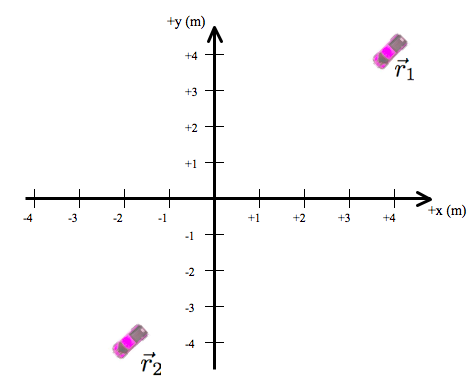
\includegraphics[scale=0.5]{uniform-motion/pickup-disp}


{\bf Answer:}

The displacement of the pickup is:

\begin{eqnarray*}
	\mbox{displacement} & = & \vectsub{r}{2} - \vectsub{r}{1}\\
	 & = &   (-2,-4)\ \meter - (+4,+4)\ \meter \\
	 & = & (-6, -8)\ \meter
\end{eqnarray*}

To sketch the displacement vector, draw an arrow from the initial position of the pickup to the final position of the pickup, as shown below.

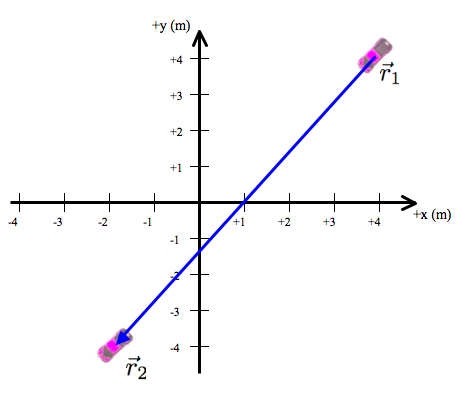
\includegraphics[scale=0.5]{uniform-motion/pickup-disp-vector}
}

\section*{Updating the position of an object}

When creating games or animation, you move objects on the screen. To move an object to some ``final'' coordinates, you take its initial coordinates and add a displacement.

\begin{eqnarray*}
	\mbox{final position coordinates} & = &  \mbox{initial position coordinates} + \mbox{displacement}
\end{eqnarray*}

Suppose that a toy pickup is at (+4,-2) m and you displace it (-3,0) m. Then, its new position is

\begin{eqnarray*}
	\mbox{final position coordinates} & = & (+4,-2) \ \meter + (-3,0)\ \meter \\
	& = & (+1,-2)\ \meter
\end{eqnarray*}

The position of the pickup at $\vectsub{r}{2}$ is shown in Figure \ref{uniform-motion/pickup-three}.

\scaledimage{uniform-motion/pickup-three}{A pickup is displaced (-3,0) m to the left.}{0.5}

\subsection*{Example}

\tightframe{

{\bf Question:}

Suppose that a toy pickup is at (+4,-2) m and you displace it (-3,0) m. Let's call this \emph{step 1}.  After two \emph{additional} steps, what will be the position of the pickup? \\

{\bf Answer:}

There is a total of three ``steps''. After the first step, the pickup is at $(+4,-2) \ \meter + (-3,0)\ \meter=(+1,-2)\ \meter$. After the second step, the pickup is at $(+1,-2) \ \meter + (-3,0)\ \meter=(-2,-2)\ \meter$, as shown in Figure \ref{uniform-motion/pickup-three}. After the third step, the pickup is at $(-2,-2) \ \meter + (-3,0)\ \meter=(-5,-2)\ \meter$. 

It is a good idea to extend the axis in Figure \ref{uniform-motion/pickup-three} and sketch the location of the pickup at $\vectsub{r}{4}$.

}

\section*{Uniform motion}

Each step of the pickup shown in Figure \ref{uniform-motion/pickup-three} takes place in a time interval $\Delta t$. If you have a running clock to measure time, then the \emph{clock reading} when the pickup is at $\vectsub{r}{1}$ is $\ssub{t}{1}$. The clock reading when the pickup is at $\vectsub{r}{2}$ is $\ssub{t}{2}$. The \emph{time interval} $\Delta t$ (or time elapsed) is defined as the difference in the clock readings:

\begin{eqnarray*}
	\Delta t & = &t_2-t_1
\end{eqnarray*}

Suppose that we use the same time interval between successive displacements. If the object's displacement in equal time intervals is the same, then the result is called \emph{uniform motion}.  It's fairly easy to identify uniform motion because successive pictures of the object in equal time intervals are equally spaced apart, as shown in Figure \ref{uniform-motion/pickup-three} for the pickup.

For example, consider a simulation of a cart moving to the right on a track shown in Figure \ref{uniform-motion/constv-cart-2}. The dots represent the location of the center of the cart at a certain clock reading. Since the clock readings were made at equal time steps and since successive positions of the cart are equally spaced, the cart's motion is described as uniform motion.

\scaledimage{uniform-motion/constv-cart-2}{A cart on a track moves to the right with uniform motion.}{0.75}

Let's record the x-positions of the cart and the clock readings in a data table.

\begin{table}[htdp]
\caption{x-positions of the cart in Figure \ref{uniform-motion/constv-cart-2}.}
\begin{center}
\begin{tabular}{|c|c|}
\hline
t (s) & x (cm)  \\
\hline
\hline
0 & 15 \\
\hline
0.1 & 25 \\
\hline
0.2 & 35  \\
\hline
0.3 & 45  \\
\hline
0.4 & 55  \\
\hline
0.5 & 65  \\
\hline
\hline
\end{tabular}
\end{center}
\label{default}
\end{table}%

A graph of x as a function of time is shown in Figure \ref{uniform-motion/constv-graph}. You will notice that a best-fit ``curve'' through the data is a straight line. The ``rise'' is 10 cm for each ``run'' of 0.1 s. This gives a constant slope for the curve. The slope is

\begin{eqnarray*}
	slope & = & \frac{rise}{run} \\
	& = & \frac{10 \ \centi\meter}{0.1\ \second} \\
	& = & 100\ \centi\meter \per \second
\end{eqnarray*}

The slope means that the x-position of the cart increases 10 cm for each 0.1 s of time elapsed, or in other words, 100 cm in each 1 second elapsed. This is called the \emph{x-velocity} of the cart. 

Note that the graph of $x$ vs. $t$ doesn't tell us anything about the y-motion of the cart. In this case, the cart is moving horizontally, so its \emph{y-velocity} is zero. As a result, we can write the velocity of the cart as  $\vect{v}=(100,0)$ cm/s. But if we didn't know its y-velocity and all we had was the data for graph for $x(t)$, then we wouldn't know anything about the y-motion of the cart.

\scaledimage{uniform-motion/constv-graph}{A graph of x-position as a function of time for the cart.}{0.4}

\pagebreak

\subsection*{Example}

\tightframe{

{\bf Question:}

A graph for the x-position as a function of time for a cart on a track is shown below. \\

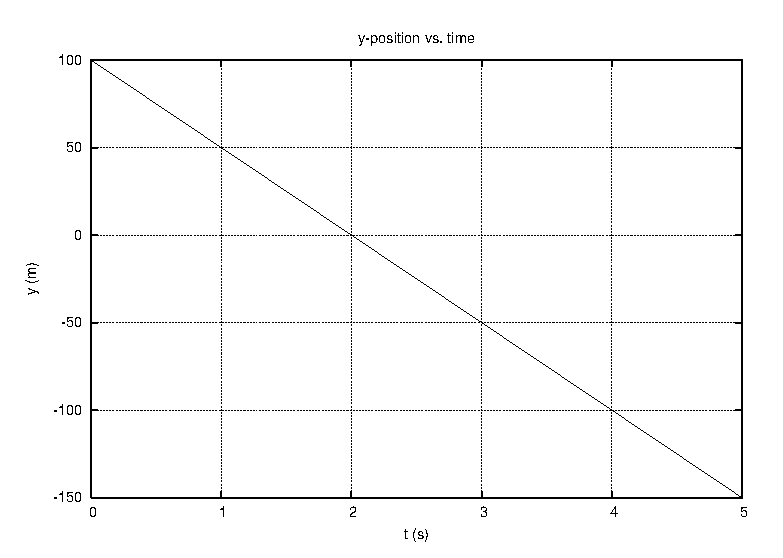
\includegraphics[scale=0.75]{uniform-motion/x-t-graph}

(a) What is the x-velocity of the cart? \\

(b) In which direction is the cart traveling? \\

(c) What can you say about the y-motion of the cart? \\

{\bf Answer:}

(a)  The x-velocity is the slope of the graph. Choose two points on the line. For example, you might choose (1 s, 20 cm) and (4 s, 5 cm).  The slop is

\begin{eqnarray*}
	slope & = & \frac{rise}{run} \\
	& = & \frac{(5-20) \ \centi\meter}{(4-1)\ \second} \\
	& = & \frac{-15 \ \centi\meter}{3\ \second} \\
	& = & -5\ \centi\meter \per \second
\end{eqnarray*}

(b) The x-velocity of the cart is negative. If we define the $+x$ axis on our coordinate system to the right, then the cart is moving to the left.

(c) This graph only tells us the x-velocity. We have no idea what the y-velocity is. Maybe the cart is traveling down a ramp, to the left. Or maybe it's traveling up a ramp, to the left. Or maybe it's traveling on a horizontal ramp. We just don't know.

}

\pagebreak

\section*{Velocity}

The velocity of an object is its displacement per second. It is calculated by

\begin{eqnarray*}
	\mbox{velocity} & = & \frac{\mbox{displacement}}{\mbox{time interval}} \\
	\vect{v} & = & \frac{\Delta \vect{r} }{\Delta t}
\end{eqnarray*}

The cart in Figure \ref{uniform-motion/constv-cart-2} has a displacement of (+10,0) cm between each dot, and the time interval between dots is 0.1 s. Thus, the cart's velocity is:

\begin{eqnarray*}
	\vect{v} & = & \frac{(+10,0)\ \centi\meter}{0.1\ \second} \\
	& = & (100,0)\ \centi\meter \per \second
\end{eqnarray*}

\section*{Predicting the future position of an object}

If you know the velocity of an object, you can calculate what its displacement will be in any given time interval. The object's displacement in a time interval $\Delta t$ is

\begin{eqnarray*}
	\mbox{displacement} & = & \mbox{velocity} \times \mbox{time interval}
\end{eqnarray*}

You can predict its future position after a time interval $\Delta t$ by adding its displacement to its initial position.

\begin{eqnarray*}
	\mbox{final position coordinates} & = &  \mbox{initial position coordinates} + \mbox{velocity} \times \mbox{time interval} \\
	\vectsub{r}{f} & = & \vectsub{r}{i} + \vect{v}\Delta t
\end{eqnarray*}

For the cart in this example, we can predict its position at any future clock reading, assuming that it continues moving with the same velocity. Since $x_i=15$ cm at $t=0$, then at $t=0.6\ \second$, 

\begin{eqnarray*}
	\ssub{x}{f} & = & \ssub{x}{i} + \ssub{v}{x}\Delta t \\
	& = & 15\ \centi\meter + (100\ \centi\meter \per \second)(0.6\ \second) \\
	& = & 75\ \centi\meter
\end{eqnarray*}

We could have used $x_i=65$ cm at $t=0.5$, then at $t=0.6\ \second$

\begin{eqnarray*}
	\ssub{x}{f} & = & \ssub{x}{i} + \ssub{v}{x}\Delta t \\
	& = & 65\ \centi\meter + (100\ \centi\meter \per \second)(0.1\ \second) \\
	& = & 75\ \centi\meter
\end{eqnarray*}

The result is the same, as long as you use the time interval $\Delta t$ since the object was at the initial x-position $x_i$.

\section*{Making things move}

In animation, you make things move one step at a time. If each step occurs in a time interval $\Delta t$, then the new position of the object after each step is:

\begin{eqnarray*}
	\mbox{new position coordinates} & = &  \mbox{current position coordinates} + \mbox{velocity} \times \mbox{time interval} \\
\end{eqnarray*}

Suppose that the time interval is $\Delta t=0.5\ \second$ and the object begins at $\vectsub{r}{i}=(4,-2)\ \meter$ and has a velocity of $(-1,2)\ \meter \per \second$. After one time step, the object will be at:

\begin{eqnarray*}
	\mbox{new position coordinates} & = &  (4,-2)\ \meter +\big((-1,2)\ \meter \per \second \big) (0.5\ \second)\\
	& = & (3.5,-1)\ \meter
\end{eqnarray*}

After the next time step, the object will be at:

\begin{eqnarray*}
	\mbox{new position coordinates} & = &  (3.5,-1)\ \meter +\big((-1,2)\ \meter \per \second \big) (0.5\ \second)\\
	& = & (3,0)\ \meter
\end{eqnarray*}

Using this method, you can continue to move the object at 0.5 s time steps. Its positions, starting at $(4,-2)$ m at 0.5 s time steps are shown in Table \ref{uniform-motion/ball-table}. The object is drawn at each time step in Figure \ref{uniform-motion/ball}.

\scaledimage{uniform-motion/ball}{Updated positions of the object from Table \ref{uniform-motion/ball-table}.}{0.4}

\newpage


\begin{table}[htdp]
\caption{Updated positions at time steps of 0.5 s for a velocity of $(-1,2)\ \meter \per \second$.}
\begin{center}
\begin{tabular}{|c|c|}
\hline
coordinates (m) & t (s) \\
\hline
\hline 
  0  & ( 4.0 , -2.0 )  \\
\hline 
  0.5  & ( 3.5 , -1.0 )  \\
\hline 
  1.0  & ( 3.0 , 0.0 )  \\
\hline 
  1.5  & ( 2.5 , 1.0 )  \\
\hline 
  2.0  & ( 2.0 , 2.0 )  \\
\hline 
  2.5  & ( 1.5 , 3.0 )  \\
\hline 
  3.0  & ( 1.0 , 4.0 )  \\
\hline 
  3.5  & ( 0.5 , 5.0 )  \\
\hline 
  4.0  & ( 0.0 , 6.0 )  \\
\hline 
  4.5  & ( -0.5 , 7.0 )  \\
\hline 
  5.0  & ( -1.0 , 8.0 )  \\
\hline
\hline
\end{tabular}
\end{center}
\label{uniform-motion/ball-table}
\end{table}%

\newpage

\subsection*{Example}

\tightframe{

{\bf Question:}

In a game, a missile starts at the location $(500,500,0)\ \meter$ at $t=0$ and travels with a constant velocity of $(-43, -25, 0)\ \meter\per\second$. Using a time step of 2.0 s, find the next 10 positions of the missile. Make a data table showing the missile's position at each clock reading.

{\bf Answer:}

After the first time step, the new position of the missile is

\begin{eqnarray*}
	\mbox{new position coordinates} & = &  \mbox{current position coordinates} + \mbox{velocity} \times \mbox{time interval} \\
	\vectsub{r}{f} & = & \vectsub{r}{i} + \vect{v}\Delta t \\
	 & = & (500,500,0)\ \meter + \big((-43, -25, 0)\ \meter\per\second \big) (2\ \second) \\
	 & = & (414,450,0) \ \meter
\end{eqnarray*}

and the clock reading is $t=0+2\ \second=2\ \second$.

After the second time step, the new position of the missile is

\begin{eqnarray*}
	\mbox{new position coordinates} & = &  \mbox{current position coordinates} + \mbox{velocity} \times \mbox{time interval} \\
	 & = & (414,450,0)\ \meter + \big((-43, -25, 0)\ \meter\per\second \big) (2\ \second) \\
	 & = & (328,400,0) \ \meter
\end{eqnarray*}

and the clock reading is $t=2+2\ \second=4\ \second$. Continue to do this for a total of 10 time steps. A data table with the results is shown below.

\begin{center}
\begin{tabular}{|c|c|}
\hline
 t (s) & coordinates (m) \\
\hline
\hline
 0 & ( 500.0 , 500.0 )  \\
\hline 
 2  & ( 414.0 , 450.0 )  \\
\hline 
 4  & ( 328.0 , 400.0 )  \\
\hline 
 6  & ( 242.0 , 350.0 )  \\
\hline 
 8  & ( 156.0 , 300.0 )  \\
\hline 
 10  & ( 70.0 , 250.0 )  \\
\hline 
 12  & ( -16.0 , 200.0 )  \\
\hline 
 14  & ( -102.0 , 150.0 )  \\
\hline 
 16  & ( -188.0 , 100.0 )  \\
\hline 
 18  & ( -274.0 , 50.0 )  \\
\hline 
 20  & ( -360.0 , 0.0 )  \\
\hline
\hline
\end{tabular}
\end{center}

}

\pagebreak

\section{Homework}

\begin{enumerate}
	\item In a certain video game that you create, an object travels diagonally from the right side to the left side. Suppose that you use real-world coordinates (not pixels) in your program, with the $+x$ axis defined to the right and the $+y$ axis defined upward. At $t=0$, an object is at $(100,200,0)$ m and has a velocity of $(-10,0,0)$ m/s. 
	
	\begin{enumerate}
		\item What is the object's displacement during a time interval of $0.1$ s?
		\item After one time step of $\Delta t=0.1\ \second$, what is the object's new position?
		\item What is the object's position at $t=5\ \second$? (Note that you can use the original position at $t=0$ and use a time interval of $5\ \second$ to find its new position.)
		\item What is the object's position at $t=10\ \second$? What about $t=15\ \second$?
	\end{enumerate}
	
	\item An object moves along the y-axis with uniform motion; its y-position as a function of time is shown in Figure \ref{uniform-motion/y-t-hw}.
	
	\scaledimage{uniform-motion/y-t-hw}{y(t) graph for an object}{0.75}
	
	\begin{enumerate}
		\item What is the y-velocity of the object?
		\item What is its y-position at $t=3$ s?
		\item What is its initial y-position (i.e. $t=0$)?
	\end{enumerate}

	\item In writing games, you will frequently make an object move at constant velocity. Suppose you are writing a \emph{Galaga} game where your spaceship moves back and forth horizontally at a constant velocity. You use real-world coordinates and a real-world coordinate system, and you choose a speed of 10 m/s for the spaceship.
	\begin{enumerate}
		\item If the spaceship is moving to the right at the given speed, what is its velocity (written as a vector)?
		\item If you use time steps of $\Delta t=0.05$ s in your animation and if the spaceship is at the position $(-50,0,0)$ m, what will be its position during the next 10 time steps? Show each calculation of each step.
	\end{enumerate}
	
\end{enumerate}


\lab{LAB:  Video Analysis of Uniform Motion}

\apparatus

\equip{Tracker software (free; download from \href{http://www.cabrillo.edu/~dbrown/tracker/}{http://www.cabrillo.edu/$\sim$dbrown/tracker/})}
\equip{video: \code{uniform-motion-ball-slow.mov} from \href{http://physics.highpoint.edu/~atitus/videos/}{http://physics.highpoint.edu/$\sim$atitus/videos/}}
\equip{video: \code{uniform-motion-ball-fast.mov} from \href{http://physics.highpoint.edu/~atitus/videos/}{http://physics.highpoint.edu/$\sim$atitus/videos/}}

\longgoal

In this experiment, you will measure and graph the x-position of a rolling steel ball as a function of time. In addition, you will learn how to use video analysis software \emph{Tracker} to measure position as a function of time for an object and find the best-fit curve to a graph.

\introduction

A video is basically a set of images recorded at a rate of 30 frames per second, or in other words a time interval of 1/30 s between frames. (However, high-speed video has a higher frame rate.) To measure an object's position in a video, you need to:

\begin{enumerate}
	\item define a coordinate system including an origin and x,y axes.
	\item define a scale; in other words define a standard length, perhaps 1 m, in the video. For this, it helps to have an object of known length, such as a meterstick, in the video. This is called a \emph{calibration}.
\end{enumerate}

%	(1) define a coordinate system including an origin and x,y axes.\\
%	\\	
%	\indent
%	(2) define a scale; in other words define a standard length, perhaps 1 m, in the video. For this, it helps to have an object of known length, such as a meterstick, in the video. \\ 
	
	It's very important that the calibration instrument, like a meterstick, is in the same plane as the object's motion. If the meterstick is closer to the camera or further from the camera than the object you are studying, then your measurement of position will be inaccurate.

Consider the object in Fig. \ref{video-uniform-motion/x-y-plane}. To measure its x-position, draw a perpendicular line from the object to the x-axis. To measure its y-position, draw a perpendicular line from the object to the y-axis.

\scaledimage{video-uniform-motion/x-y-plane}{Position of an object depends on the origin and scale of the coordinate system.}{0.5}


\smallframe{Using the 1 m scale shown in the image, estimate the (x,y) coordinate of the object and use this to calculate the approximate distance of the object from the origin in Fig. \ref{video-uniform-motion/x-y-plane}}

Video analysis software makes it easy to measure position coordinates (both x and y) and time for an object. After defining the scale and the coordinate system, you click on the object. The software shows a dot where you clicked and advances the video to the next frame. The software measures the position of where you clicked in units of pixels and then uses the calibration and your definition of the coordinate system to convert this position in pixels to a position in meters (or whatever units are used in the calibration).

The software also measures time because it knows that the video is recorded at 30 frames per second (or perhaps higher for high-speed video). Thus, whenever you advance the video, time advances 1/30 s. With time and position measured by the software, you can calculate velocity by numerically calculating the derivative of the position with respect to time. Other variables can also be calculated and graphed. All of these calculations can be done by the software.

%Suppose an object moves with uniform motion in the +x direction. Fig. \ref{video-uniform-motion/motion-map} shows an object at intervals of 1/30 s between the first image on the left and the last image  on the right.

%\scaledimage{video-uniform-motion/motion-map}{Position of an object at equal time intervals of 1/30 s.}{0.8}

%\tightframe{Suppose that we define $t=0$ to occur at the initial position of the object (the left image). In Fig. \ref{video-uniform-motion/motion-map}, label the time $t$ for each subsequent position of the object.}

%\bigframe{Measure the x-position of the object from the first image to the last image. Define the origin $x=0$ to be the position of the object at $t=0$.  Make a data table below showing x-position ($x$) and time ($t$) for the object.
%}

%\smallframe{By examining the x-coordinate of the object as a function of time, is the x-motion characterized by uniform motion or non-uniform motion (speeding up or slowing down, for example)? Give a reason for your answer.}

%\medframe{Sketch a graph of x vs. t for the object. No numbers are needed.}

%\medframe{If the object instead moves to the left and if the origin is defined to be the furthest image on the right, what would the graph look like? }

\procedure

\begin{enumerate}
	\item Download the file \file{constant-velocity-slow.mov} from the given web site by right-clicking on the link and choosing {\bf Save As...} to save it to your desktop.
	\item Open the \file{Tracker} software on your computer.
	\item Use the menu \menu{Video$\to$Import...} to import your video, as shown in Figure \ref{video-uniform-motion/video-import}.

\scaledimage{video-uniform-motion/video-import}{Video$\to$Import menu}{0.5}
	
	\item To zoom in or out on the video, click on the toolbar's magnifying glass icon that is shown in Figure \ref{video-uniform-motion/zoom}. When it appears with a \button{+}, then clicking once on the video will zoom in (thus making it larger).  Clicking the magnifying glass again will make it \button{--}; then clicking on the video will zoom out (thus making it smaller). Zoom in and out on the video to see how it works.
	
\scaledimage{video-uniform-motion/zoom}{The icon used to expand the video.}{1}	
	
	\item At this point, it's nice to lay out the video and graphs so that you can clearly see everything. The middle border between panes, seen in Fig. \ref{video-uniform-motion/page-arrange}, can be dragged left and right to make the video pane smaller and graphs larger. The same is true of any other bar that separates panes in the window.
	
	\scaledimage{video-uniform-motion/page-arrange}{Drag the vertical or horizontal bars the make panes larger or smaller.}{0.4}
		
	\item Note the video controls at the bottom of the video pane. Go ahead and play the video, step it forward, backward, etc. in order to learn how the video controls work. Note the counter that merely shows the frame number for any frame. Also, click on each of the icons in the video control bar to see what they are used for. Finally, use the left and right arrow keys on your keyboard, and note that they can be used to control the video as well.

	\item Rewind to the first frame of the video. This is the instant that you will begin making measurements of the position of the moving object.
	
	\item Since the ball moves fairly slowly on the track, we can skip frames between marking the ball and thus take fewer data points. Click on the \menu{Step Size} button, as shown in Figure \ref{video-uniform-motion/step-size} and change it to {\bf 5}.
	
\scaledimage{video-uniform-motion/step-size}{Change the step size in order to skip frames.}{0.5}
	
	\item You now need to define the origin of the coordinate system. In the toolbar, click the \menu{Axes} icon shown in Fig. \ref{video-uniform-motion/coord-icon} to show the axes of the coordinate system. (By now, you have probably noticed that you can hover the mouse over each icon to see what they do).
	
	\image{video-uniform-motion/coord-icon}{Icon used to set the coordinate system axes.}

	\item Click and drag on the video to place the origin of the coordinate system at the location where you would like to define (0,0), as shown in Figure \ref{video-uniform-motion/coord-sys}. You can place the origin at any point you choose, but in this case, it makes sense to put the origin at the location of the ball in the first frame being analyzed. 
		
	\scaledimage{video-uniform-motion/coord-sys}{Click and drag to set the origin of the coordinate system}{0.5}
	
	\item If you click the x-axis and drag, you can rotate the coordinate system. In this case, the video camera was not level; therefore, rotate the x-axis until it is parallel to the track.
	
	\item Click the \menu{Axes} tool again to hide the axes from the video pane. You can click this icon at any time to show or hide the axes.

	\item Now, you must calibrate distances measured in the video. In the toolbar, click on the \menu{Tape Measure} icon shown in Figure \ref{video-uniform-motion/ruler} to set the scale for the video.
		
	\scaledimage{video-uniform-motion/ruler}{Icon used to set the scale.}{1}

	\item A blue double-sided arrow will appear. Move the left end of the arrow to the left end of the track, and move the right end of the arrow to the right end of the track. Double-click the number that is in the center of the arrow, and enter the length of the track, 2.2. (Our units are meters, but Tracker does not use units. You must remember that the number 2.2 is given in meters.) The scale will appear as shown in Figure \ref{video-uniform-motion/set-scale}.

	\scaledimage{video-uniform-motion/set-scale}{Enter the length of the track.}{0.6}
	
	\item Click the tape measure icon again to hide the blue scale from the video.

	\item You are ready to add markers to the video to mark the position of the ball. Let's not show the coordinate system and scale. It's too distracting. So, make sure you've clicked the \menu{Axes} and \menu{Tape Measure} icons in the toolbar to hide them.
		
	\item To add markers, click on the \button{Create} button and select \menu{Point Mass} as shown in Figure \ref{video-uniform-motion/add-markers}. Then, {\bf mass A} will be created, and a new $x$ vs. $t$ graph will appear in a different pane. You will now be able to mark the position of the ball which will be referred to as {\bf mass A}.

	\scaledimage{video-uniform-motion/add-markers}{The Track Control toolbar.}{0.5}
	
	\item We will want to set the frame step size to 5 so that it will skip 4 frames every time we step forward in the video. Double check that the step size is 5 in the video control toolbar.

	\item  {\bf To mark the center of the ball, hold the SHIFT key down and click once on the center of the ball.} You should notice that a marker appears at the position of the ball where you clicked and that the video advances one step.
	
	\item Again, shift-click on the ball to mark its position. You should now see two marks.
	
	\item Continue marking the position of the ball until it reaches the right end of the track. Note that only a few of the marks are shown in the video pane. To display all of the marks or a few of the marks or none of the marks, use the \menu{Set Trail Length} icon shown in Figure \ref{video-uniform-motion/set-trail}. Clicking this icon continuously will cycle through no trail, short trail, and full trail which will show you no marks, a few marks, or all marks. 

	\scaledimage{video-uniform-motion/set-trail}{The Set Trail icon is used to vary the number of marks shown.}{1}
	
	
	 After marking the ball as it moves from the left end to the right end of the track, your video should look like the picture shown in Fig. \ref{video-uniform-motion/final-dots} if you have set the trail length to show the full trail.
		
	\scaledimage{video-uniform-motion/final-dots}{Marks showing the ball's position.}{0.4}
		
	\item Tracker uses the frame and frame rate to calculate $t$, and it uses the scale and coordinates of the marks to calculate $x$ and $y$ coordinates for the ball. It uses numerical differentiation to calculate x-velocity and y-velocity.
\end{enumerate}

\analysis

\subsection*{$x$ vs. $t$ graph}

\begin{enumerate}
	\item We will now analyze the $x$ vs. $t$ graph. You can click and drag the border of the video pane to make it smaller so that you can focus on the graph.
	\item Play the video. (You can hide the marks if you wish by clicking the \menu{Show or hide positions} icon, and you can show the path by clicking the \menu{Show or hide paths} icon. Both of these icons are in the toolbar.) Note how the graph and video are synced. Each video frame data point is shown in the graph using a filled rectangle.
	
	Also, when you click on a data point on the graph, the video moves to the corresponding frame.
	
	\item Observe the $x$ vs. $t$ graph.
		
	\tinyframe{Describe in words the type of function that describes this graph of x vs. t? (i.e. linear, quadratic, square root, sinusoidal, etc.)}
	
	\item  Right-click (or ctrl-click) on the graph and select \menu{Analyze...}. In the resulting window, check the checkbox for \menu{Fit}, and additional input boxes will appear, as shown in Figure \ref{video-uniform-motion/curve-fit}. The Fit Name should be ``Line'' and the equation will be $x=a*t+b$ where $a$ is the slope and $b$ is the vertical intercept. Check the checkbox for \menu{Autofit} and the best-fit line will appear in the graph.
	
	\scaledimage{video-uniform-motion/curve-fit}{The Data Tool for finding the best-fit curve for the data.}{0.5}
	
	
	\smallframe{Record the function and the values of the constants for your curve fit. Write the function for x(t), with the appropriate constants (also called fit parameters).}

	\smallframe{In general, what does the slope of the x vs t graph tell you? (Consider its units. Your answer should be a sentence, not a number.) }
	
	\smallframe{From the curve fit parameters, determine the x-velocity of the ball.}
	
\subsection*{$v_x$ vs. $t$ graph}

	
	\item Now, we will look at the x-velocity vs. time graph.
	
	\smallframe{What do you expect the x-velocity vs. time graph to look like? Sketch your prediction below.}
	
	
	\item Close the Data Tool window and return to the main window. Click once on the vertical axis label and change it from $x$ to $vx$, as shown in Figure \ref{video-uniform-motion/x-velocity}.
	
	\scaledimage{video-uniform-motion/x-velocity}{Changing the variables plotted on the graph.}{0.4}
		
	
Note that the data appears to be all over the place. That's because by default, the graph is ``zoomed in'' on the data. If you examine the numbers on the vertical axis, you'll notice that the data probably lies between 0.3 m/s and 0.35 m/s (though your data might also vary from mine). That's a very small variation in the velocity during the 5-second time interval that the ball is moving. And the variation is likely due to measurement error such as not clicking exactly on the center of the ball for every mark.
	
	\item Hover over the lowest part of the vertical axis (near the graph's origin, on the vertical axis). Click once and change the minimum on the vertical scale to 0. Do the same thing at the top of the scale and change the maximum to 0.5. The data now appears to be along a horizontal line, though there is some scattering in the data due to uncertainty in the measurements, as shown in Figure \ref{video-uniform-motion/velocity-data}.
	
	\scaledimage{video-uniform-motion/velocity-data}{The x-velocity vs. time graph.}{0.4}
	
	\item Right-click (or ctrl-click) on the graph and select \menu{Analyze...} in order to analyze the $v_x$ vs. $t$ graph. You may notice that the data for both $x$ and $v_x$ are displayed on the same graph. If this occurs, uncheck the checkboxes for $x$ in the upper right corner of the window.  
	
	\item Once again, change the minimum and maximum values on the scale so that the graph is not zoomed in on the data. Do an auto-fit. 
	
	\smallframe{Record the fit constants and equation for the curve fit. From the curve fit, determine the initial x-velocity.}
	
	\smallframe{You will notice a slight downward slope of this graph. What does this tell you? Answer in a complete sentence.}
	
	\item Since the x-velocity is nearly constant, we would like to have an average of the x-velocity measured at each instant. Thus, check the checkbox for \menu{Statistics}.
	
	\smallframe{Record the mean x-velocity and the standard deviation.}
	
	\smallframe{Is the slope of the $x$ vs. $t$ graph within $\overline{v_x}\pm \sigma$?}

	\item Be sure to save the Tracker file in the same folder as your video. Transfer this file and the video to a USB thumb drive for your records. In fact, it is best to save as you go. {\bf \emph{Remember, save early and often!}}
	
\end{enumerate}

\report

\begin{description}

\item[C]  Complete the experiment and report your answers for the following questions.

\begin{enumerate}
	 \item If you were to only see the marks in the video and not see any graphs, how would you know that it is uniform motion (as opposed to non-uniform motion)?
	\item What is the x-velocity of the ball as measured by the slope of your graph of x vs. t?
	\item What is the x-velocity of the ball as measured by the average of the values of $v_x$ on the graph of $v_x$ vs. $t$?
	\item When you found the mean value of $v_x$, you also recorded the standard deviation. What was the standard deviation and did your results reported in parts (2) and (3) agree within this standard deviation?
\end{enumerate}

\item[B] Do all parts for {\bf C}, analyze the motion of the ball in the video \file{constant-velocity-fast.mov} and answer the following questions.

\begin{enumerate}
 \item What is the x-velocity of the ball as determined from the $x$ vs. $t$ graph?
 \item What is the average and standard deviation of the x-velocity of the ball as determined from the $v_x$ vs. $t$ graph?
\end{enumerate}

\item[A] Do all parts for {\bf B} and answer the following questions. Note that you can make a sketch using a ruler. You don't have to use graph paper. However, you may use graph paper or a computer to do your sketches.

\begin{enumerate}

 \item Car A travels with a constant x-velocity of 30 mph for two hours, and Car B travels with a constant x-velocity of 60 mph for two hours. Each of them start at the origin at $t=0$. On the same set of axes, sketch a graph of $x$ vs. $t$ for each car. (There should be two lines on your graph. Be sure to label the axes with correct units.)
% \item For the cars in the previous question, sketch a graph of $v_x$ vs. $t$ for the two cars on the same set of axes.
 \item Suppose that the ball in the video started at the right end of the track and traveled with a constant velocity to the left. If the origin is set at the left end of the track with the $+x$ axis pointing to the right (just as before), sketch a graph of $x$ vs. $t$ for the ball.
% \item What would a graph of $v_x$ vs. $t$ look like for the ball in the previous question?
 \item Suppose that the ball in the video started at the right end of the track and traveled with a constant velocity to the left. If the origin is set at the right end of the track with the $+x$ axis pointing to the right, sketch a graph of $x$ vs. $t$ for the ball.
% \item What would a graph of $v_x$ vs. $t$ look like for the ball in the previous question?
\end{enumerate}
\end{description}


%Key%

%C

%1.  The marks are evenly spaced.
%2.  0.319 m/s
%3.  0.318 m/s
%4.  0.015 m/s

%B

%1.  0.529 m/s
%2.  0.526 +- 0.016 m/s

%A

%1. Car B has twice the slope as Car A.
%2. Slope is negative. y-intercept is at 2 m.
%3. Slope is negative. y-intercept is at 0.


\lab{PROGRAM -- Uniform Motion}

\apparatus
\equip{Computer}
\equip{GlowScript -- www.glowscript.org}

\longgoal

The purpose of this activity is to learn how to use GlowScript (VPython) to model uniform motion (i.e. motion with a constant velocity).

\introduction

\subsection*{General structure of a program}

In general, every program that models the motion of physical objects has two main parts:

\begin{enumerate}
	\item {\bf Before the loop}:  The first part of the program tells the computer to:
	\begin{enumerate}
		\item Create 3D objects.
		\item Give them initial positions and velocities.
		\item Define numerical values for constants we might need.
	\end{enumerate}
	\item {\bf The \texttt{while} loop}:  The second part of the program, the loop, contains the lines that the computer reads to tell it how to update the positions of the objects over and over again, making them move on the screen. \end{enumerate}

To learn how to model the motion of an object, we will write a program to model the motion of a ball moving with a constant velocity.

\procedure

Before you begin, it will be useful to look back at your notes or a previous program to see how you created a sphere and box.

\begin{enumerate}

	\item Create a new program in GlowScript and save this file with a new name like \texttt{ball-uniform-motion}.

\item Add the line below to create a track that is at the origin and has a length of 3 m, a height of 0.05 m, and a width of 0.1 m. Note that the y-position is -0.075 m (below zero) so that we can place a ball at $y=0$ such that it appears to be on top of the track..

\begin{myvpython}
track=box(pos=vector(0,-0.075,0), size=vector(3,0.05,0.1), color=color.white)
\end{myvpython}

\item Create a ball (i.e. sphere) at the position $(-1.4,0,0)\ \meter$. Choose its radius to be an appropriate size so that the ball appears to be on top of the track and name it \code{ball}.

\item Run your program. The ball should appear to be on the top of the track and should be on the left side of the track as shown in Figure \ref{vpython-uniform-motion/track}.

\scaledimage{vpython-uniform-motion/track}{A ball on a track.}{0.5}

Now, we will define the velocity of the ball to be to the right with a speed of 0.3 m/s. A unit vector that points to the right is (1,0,0). So, the velocity of the ball can be written on paper as:

\begin{eqnarray*}
	\vect{v} & = & \vectmag{v}\hat{v} \\
	& = & 0.3*(1,0,0) 
\end{eqnarray*} 

Next we will see how to write this in VPython.

\item Just as the position of the ball is referenced as \code{ball.pos}, let's define the ball's velocity as \code{ball.v} which indicates that v is a property of the object named \code{ball}.  To do all of this, type this line at the end of your program.
	
\begin{myvpython}
ball.v=0.3*vector(1,0,0)
\end{myvpython}

This statement creates a property of the ball  \code{ball.v} that is a vector quantity with a magnitude 0.3 that points to the right. 

\item Whenever you want to refer to the velocity of the ball, you must refer to \type{ball.v}. For example, type the following at the end of your program.

\begin{myvpython}
print(ball.v)
\end{myvpython}

\item When you run the program, it will print the velocity of the ball as a 3-D vector as shown below:

\begin{verbatim}
<0.3, 0, 0>
\end{verbatim}

\subsection*{Define values for constants we might need}

%To make the cart move, we calculate its new position after each time interval $\Delta t$ using the equation:
% 
%\begin{eqnarray*}
%	\mbox{new position coordinates} & = &  \mbox{current position coordinates} + \mbox{velocity} \times \mbox{time interval} \\
%\end{eqnarray*}
 
To make an object move, we will update its position every $\Delta t$ seconds. In general, $\Delta t$ should be small enough such that the displacement of the object is small. The size of $\Delta t$ also affects the speed at which your program runs. If it is exceedingly small, then the computer has to do lots of calculations just to make your object move across your screen. This will slow down the computer.

\item For now, let's use 1 hundredth of a second as the time step, $\Delta t$. At the end of your program, define a variable $dt$ for the time interval.

\begin{myvpython}
dt=0.01
\end{myvpython}

\item Also, let's define the total time $t$ for the clock. The clock starts out at $t=0$, so type the following line.

\begin{myvpython}
t=0
\end{myvpython}

That completes the first part of the program which tells the computer to:

	\begin{enumerate}
		\item Create the 3D objects and name them.
		\item Give the ball an initial position and velocity.
		\item Define variable names for the clock reading $t$ and the time interval $dt$.
	\end{enumerate}
	
\subsection*{Create a ``while" loop to continuously calculate the position of the object.}

We will now create a \code{while} loop. Each time the program runs through this loop, it will do two things:

	\begin{enumerate}
		\item Calculate the displacement of the ball and add it to the ball's previous position in order to find its new position. This is known as the ``position update''.
		\item Calculate the total time by incrementing $t$ by an amount $dt$ through each iteration of the loop.
		\item Repeat.
	\end{enumerate}

	\item For now, let's run the animation for 10.0 s. On a new line, begin the \code{while} statement as shown below. This tells the computer to repeat these instructions as long as $t < 10.0$ s.
	
\begin{myvpython}
while t < 10.0:
\end{myvpython}
	
	Make sure that the \type{while} statement ends with \type{:} because Python uses this to identify the beginning of a loop. 
	
	To understand what a while loop does, let's update and then  print the clock reading.

\item Below the \code{while} statement, add the following line. Note that it must be indented.

\begin{myvpython}
	t=t+dt
\end{myvpython}

After adding this line, your \code{while} loop will look like:

\begin{myvpython}
while t < 10.0:
	t=t+dt
\end{myvpython}

Note that this line takes the clock reading $t$, adds the time step $dt$, and then assigns the result to the clock reading. Thus, through each pass of the loop, the program updates the clock reading.

\item Print the clock reading by typing the following line at the end of the while loop (again, make sure it's indented) and run your program.

\begin{myvpython}
	print(t)
\end{myvpython}

After adding the \code{print} statement, check that your \code{while} loop looks like:

\begin{myvpython}
while t < 10.0:
	t=t+dt
	print(t)
\end{myvpython}

\item Run the program. View the clock readings printed below the 3D scene.

\item You can make it run indefinitely (i.e. without stopping) by saying ``while true''  so you can change the \code{while} statement to read:

	\begin{verbatimtab}
	while 1:
		rate(100)
	\end{verbatimtab}	

The \code{rate(100)} statement tells the computer to try to run the loop 100 times in one second.

Check that your program (loop) now looks like:

\begin{myvpython}
while 1:
	rate(100)
	t=t+dt
	print(t)
\end{myvpython}

\item Run the program.  Now, it will print clock readings continually until you click the  {\bf Edit this program} link and return to the editor.

\tightframe{Stop and reflect on what is going on in this \code{while} loop. Your understanding of this code is essential for writing games.}

Just as we updated the clock using \code{t=t+dt}, we also want to update the object's position. Physics tells us that the object's new position is given by:

\begin{eqnarray*}
	\mbox{new position coordinates} & = &  \mbox{current position coordinates} + \mbox{velocity} \times \mbox{time step} \\
	\vec{r}_f & = & \vec{r}_i + \vec{v}\Delta t 
\end{eqnarray*}

This is called the \emph{position update equation}. It says, ``take the current position of the object, add its displacement, and the result is the new position of the object.'' In VPython the ``='' sign is an \emph{assignment} operator. It takes the result on the right side of the = sign and assigns its value to the variable on the left. 

Now we will update the ball's position after each time step \code{dt}.

\item Inside the \code{while} loop \emph{before you update the clock}, update the position of the ball by typing:

\begin{myvpython}
	ball.pos=ball.pos+ball.v*dt
\end{myvpython}

After typing this line, check that your \code{while} loop looks like:

\begin{myvpython}
while 1:
	rate(100)
	ball.pos=ball.pos+ball.v*dt
	t=t+dt
	print(t)
\end{myvpython}

\item Change the print statement to print both the clock reading and the position of the ball. Separate the variables by commas as shown:

\begin{myvpython}
	print(t, ball.pos)
\end{myvpython}

\item Run your program. You will see the ball move across the screen to the right. Because we have an infinite loop, it will continue to move to the right until you return to the editor. After the ball travels past the edge of the track, the camera will zoom backward to keep all of the objects in the scene.

\item Printing the values of the time and the ball's position may slow down the computer. Comment out your print statement by typing the \# sign in front of the \code{print} statement (as in \code{\#print)}. Run your program again. 

Sometimes you need to print data in order to check the computer's calculations. However, it can also be distracting and unnecessary. In general, print when you need to check the computer's calculation and debug your program. Otherwise, don't print.

\item Adjust the \code{rate} statement and try values of 10 or 200, for example. How does increasing or decreasing the argument of the rate function affect the animation?

The \code{rate(100)} statement specifies that the while loop will not be executed more than 100 times per second, even if your computer is capable of many more than 100 loops per second. (The way it works is that each time around the loop VPython checks to see whether 1/100 second of real time has elapsed since the previous loop. If not, VPython waits until that much time has gone by. This ensures that there are no more than 100 loops performed in one second.)

If you want time to advance in the simulation at the same rate as a real clock (meaning, as nearly as possible, the simulation time is equal to real time), then set the values of \code{dt} and \code{rate()} so the product is equal to one. For example, if \code{dt=0.01}, then choose \code{rate(100)} because $0.01 * 100 = 1$. Or if \code{dt=0.02}, then choose \code{rate(50)}.

\end{enumerate}

\ \\

\newpage


\analysis

\begin{description}

\item[C] Do all of the following.
\begin{enumerate}
	\item Start a new program in GlowScript and save this file with a new name like \texttt{ball-uniform-motion-C}.
	\item Copy the code from your previous program and paste it into this new program.
	\item Simulate the motion of a ball that starts on the right end of the track and travels to the left with a speed of 0.5 m/s for 5 s. The ball's initial position should be $(1.5,0,0)$ m. The \code{while} loop should run while $t<5$ s. Print the time and position of the ball.
\end{enumerate}

\item[B] Do everything for {\bf C} and the following.

\begin{enumerate}
	\item Start a new program in GlowScript and save this file with a new name like \texttt{ball-uniform-motion-B}.
	\item Create two balls on a track:  Ball A starts on the left side at $(-1.5,0,0)$ m and Ball B starts on the right side at  $(1.5,0,0)$ m. Name them \code{ballA} and \code{ballB} in your program.
	\item Ball A travels to the right with a speed of 0.3 m/s and Ball B travels to the left with a speed of 0.5 m/s. Define each of their velocities as \code{ballA.v} and \code{ballB.v}, respectively.
	\item Set the \code{while} loop to run while $t<5$ s. 
	\item Print the clock reading \code{t} and the position of each ball up to $t=5$ s.
	\item At what clock reading $t$ do they pass through each other?
\end{enumerate}

\item[A] Do everything for {\bf B} and the following.

\begin{enumerate}
	\item Start a new program in GlowScript and save this file with a new name like \texttt{ball-uniform-motion-A}.
	\item Create a similar track as before, but with the width as 3 m. When the scene is rotated, the track appears as a table top.
	\item Create three balls that all start at $x=-1.5, y=0$; however, stagger their z-positions so that one travels down the middle of the table, one travels down one edge of the table, and the other travels down the other edge of the table. Name them \code{ballA}, \code{ballB}, and, \code{ballC}, respectively, and give them different colors.
	\item Set the x-velocities of the balls to: (A) 0.25 m/s, (B) 0.5 m/s, and (C) 0.75 m/s.
	\item At what time does Ball C reach the end of the table? (Use a print statement to determine this.)
	\item What are the positions of all three balls when Ball C reaches the end of the table? (Use a print statement to determine this.)
\end{enumerate}

\end{description}


\lab{PROGRAM -- Lists, Loops, and Ifs}

\apparatus
\equip{Computer}
\equip{VPython -- www.vpython.org}

\longgoal

The purpose of this activity is to learn how to use lists, \code{for} loops, and \code{if} statements in VPython.

\introduction

\subsection*{Lists and For Loops}

When writing a game, you will typically have multiple objects moving on a screen at one time. As a result, it is convenient to store the objects in a list. Then, you can loop through the list and for each object in the list, update the position of the object.

\procedure

Before you begin, it will be useful to look back at your notes or a previous program to see how you create objects such as spheres and boxes and how you make objects move. These instructions do not repeat the VPython code that you learned in previous activities. Have those chapters and programs available for reference as you do this activity.

\begin{enumerate}

	\item Open a new window in VIDLE. 
	
	\item Enter the following statement in the IDLE editor window.
	
\begin{myvpython}	
from visual import *
\end{myvpython}

\item Save this file with a new name like \texttt{move-objects.py}.

\subsection*{The \code{for} loop and the \code{range()} list}

\item Type the \code{for} loop shown below.

\begin{myvpython}
for i in range(0,10,1):
    print(i)
\end{myvpython}
    
\item Save and run your program. The program should print:

\begin{verbatim}
>>> 
0
1
2
3
4
5
6
7
8
9
\end{verbatim}

The statement \code{range(0,10,1)} creates a list of numbers: \code{0, 1, 2, 3, 4, 5, 6, 7, 8, 9}. The \code{for} loop goes through this list, one item at a time, starting with the first item. For each \emph{iteration} through the loop, it executes the code within the loop, but the value of \code{i} is replaced with the item from the list. Thus the value of \code{i} will first have the value of 0. Then for the next iteration of the loop, it has the value 1. The loop continues until it has accomplished 10 iterations and \code{i} has taken on the values of 0 through 9, respectively. Note that the number 10 is not in the list.

\item Change the arguments in the \code{range(0,10,1)} function. Change 0 to 5, for example. Or change 1 to 2. You can even change the 1 to --1 to see what this does. Run the program each time you change one of the arguments and figure out how each argument affects the resulting list. Write your answers below.

\tightframe{In the function  \code{range(0,10,1)}, how does changing each argument affect the resulting list of numbers?\\

0:  \\

10: \\

1: \\
}

\item Delete the entire \code{for} loop for now, and we'll come back to it later.

\subsection*{Lists}

When writing games, you may have a lot of moving objects. As a result, it is convenient to store your objects in a list. Then you can loop through your list and move each object or check for collisions, etc.

\item To show how this works, first create 4 balls that are all at $x=-5, z=0$. However, give them y values that are $y=-3, y=-1, y=1, y=3$, respectively. Name them \texttt{ball1}, \texttt{ball2}, etc. Give them different colors and make their radius something that that looks good on the screen. 

\item Run your program to verify that you have four balls at the given locations. The screen should look like Figure \ref{vpython-lists-and-ifs/4-balls} but perhaps with a black background and different color balls.

\scaledimage{vpython-lists-and-ifs/4-balls}{Four balls}{0.5}

\item Define the balls' velocity vectors such that they will all move to the right but with speeds of 0.5 m/s, 1 m/s, 1.5 m/s, and 2 m/s. Remember that to define a ball's velocity, type:

\begin{myvpython}
ball1.v=0.5*vector(1,0,0)
\end{myvpython}

You'll have to do this for all four balls. Be sure to change the name of the object and speed. You should have four different lines which specify the velocities of the four balls.

Now we will create a list of the four balls. VPython uses the syntax: \code{[item1, item2, item3,...]} to create a list where item1, item2, etc. are the list items and the square brackets [] denote a list. These items can be integers, strings, or even objects like the balls in this example.

\item To create a list of the four balls, type the following line at the end of your program.

\begin{myvpython}
ballsList = [ball1, ball2, ball3, ball4]
\end{myvpython}

Notice that the names of the items in our list are the names we gave to the four spheres. The name of our list is \code{ballsList}. We could have called the list any name we wanted.

\subsection*{Motion}

We are going to make the balls move. Remember, there are three basic steps to making the objects move.

\begin{itemize}
	\item Define variables for the clock and time step.
	\item Create a \code{while} loop.
	\item Update the object's position and update the clock reading.
\end{itemize}

\item Define variables for the clock and for the time step.

\begin{myvpython}
t=0
dt=0.01
\end{myvpython}

\item Create an infinite \code{while} loop and use a \code{rate()} statement to slow down the animation.

\begin{myvpython}
while 1:
    rate(100)
\end{myvpython}

\item We are now ready to update the position of each ball. However instead of updating each ball individually, we will use a \code{for} loop and our list of balls. Type the following loop to update the position of each ball. Note that it should be indented.

\begin{myvpython}
    for thisball in ballsList:
        thisball.pos=thisball.pos+thisball.v*dt    
\end{myvpython}

This loop will iterate through the list of balls. It begins with \texttt{ball1} and assigns the value of \texttt{thisball} to \texttt{ball1}. Then, it updates the position of \texttt{ball1} using its velocity. On the next iteration, it uses \texttt{ball2}. After iterating through all objects in the list, it completes the loop. And at this point it has updated the position of each ball.

\item Now update the clock. Your while loop  should ultimately look like the following:

\begin{myvpython}
while 1:
    rate(100)
    for thisball in ballsList:
        thisball.pos=thisball.pos+thisball.v*dt    
    t=t+dt
\end{myvpython}

Note that the line \code{t=t+dt} is indented beneath the \code{while} statement but is not indented  beneath the \code{for} loop. As a result, the clock is updated upon each iteration in the while loop, not the for loop. The for loop merely iterates through the balls in the ballsList.

Using a \code{for} loop in this manner saves you from having to write a separate line for each ball. Imagine that if you had something like 20 or 50 balls, this would save you a lot of time writing code to update the position of each ball.

\item Run your program. You should see the four balls move to the right with different speeds.

\item When a ball reaches the right side of the window, the camera will automatically zoom out so that the scene remains in view. In game, we wouldn't want this. Therefore, let's set the size of our window and tell the camera not to zoom. Near the beginning of your program, after the \code{import} statement, add the following lines:

\begin{myvpython}
scene.range=5
scene.autoscale=False
\end{myvpython}

The range attribute of \code{scene} sets the right edge of the window at $x=+5$ and the left edge at $x=-5$. The autoscale attribute determines whether the camera automatically zooms to keep the objects in the scene. We set autoscale to false in order to turn it off. Set it to true if you want to turn on autoscaling.

\item Run your program.

\subsection*{IF statements}

We are going to keep the balls in the window. As a result, our code must check to see if a ball has left the window. If it has, then reverse the velocity. When you need to check \emph{if} something has happened, then you need an \code{if} statement.

Let's check the x-position of the ball. If it exceeds the edge of our window, then we will reverse the velocity. If the x-position of a ball is greater than $x=5$ or is less than $x=-5$, then multiply its velocity by $-1$. Though we can write this with a single \code{if} statement, it might make more sense to you if we use the \emph{if-else} statement. The general syntax is:

\begin{verbatim}
if condition1 :
    indentedStatementBlockForTrueCondition1
elif condition2 :
    indentedStatementBlockForFirstTrueCondition2
elif condition3 :
    indentedStatementBlockForFirstTrueCondition3
elif condition4 :
    indentedStatementBlockForFirstTrueCondition4
else:
    indentedStatementBlockForEachConditionFalse
\end{verbatim}

The keyword ``elif'' is short for ``else if''. There can be zero or more \code{elif} parts, and the \code{else} part is optional.

\item After updating the velocity of each ball inside the \code{for} loop, add the following \code{if-elif} statement:

\begin{myvpython}
        if thisball.pos.x>5:
            thisball.v=-1*thisball.v
        elif thisball.pos.x<-5:
            thisball.v=-1*thisball.v
\end{myvpython}

Note that it should be indented inside the \code{for} loop because you need to check each ball in the list.

After inserting your code, your \code{while} loop should look like:

\begin{myvpython}
while 1:
    rate(100)
    for thisball in ballsList:
        thisball.pos=thisball.pos+thisball.v*dt
        if thisball.pos.x>5:
            thisball.v=-1*thisball.v
        elif thisball.pos.x<-5:
            thisball.v=-1*thisball.v
    t=t+dt
\end{myvpython}

\item Run your program. You should see each ball reverse direction after reaching the left or right edge of the scene.

\end{enumerate}

\ \\

\newpage


\analysis

\begin{description}

\item[C] Do all of the following.
\begin{enumerate}
	\item Start with your program from this activity and save it as a different name.
	\item When a ball bounces off the right side of the scene, change its color to yellow. 
	\item When a ball bounces off the left side of the scene, change its color to magenta.
\end{enumerate}

\item[B] Do everything for {\bf C} and the following.

\begin{enumerate}
	\item Create 10 balls that move horizontally and bounce back and forth within the scene. Make the scene 10 units wide and give the balls initial positions of $x=-10$, and $z=0$, but with $y$ positions that are equally spaced from $y=0$ to $y=9$. Give them different initial velocities. Make their radii and colors such that they can be easily seen but do not overlap.
\end{enumerate}

\item[A] Do everything for {\bf B} with the following modifications and additions.

\begin{enumerate}
	\item Start with your program in part (B) with 10 balls that start at the same positions as in part B ($x=-10$ and $z=0$, with $y$ positions that are equally spaced from $y=0$ to $y=9$).
	\item Set the initial velocity of each ball to be identical. Give them the same speed, but set their velocities to be in the $-y$ direction.
	\item When a ball reaches the bottom of the scene ($y=-10$), change its velocity to be in the $+x$ direction. When a ball reaches the right side of the scene change its velocity to be in the $+y$ direction. When a ball reaches the top of the scene, change its velocity to be in the $-x$ direction. Finally, when it reaches the left side of the scene, change its velocity to be in the $-y$ direction. In this way, make the balls move around the edge of the scene.\\
	\item Run your program. You might find that the balls do not move as you expect. The reason is that if you update a ball's position and it just barely goes out of the scene, then you need to move the ball back within the scene. For example, in the python code below, if the ball's position is updated and it goes past the right edge of the scene at $x=10$, then the line within the IF statement moves the ball one step backward, back into the scene again. In other words, it reverses the position update statement. (Note the negative sign.)

\begin{myvpython}
        thisball.pos=thisball.pos+thisball.v*dt
        if thisball.pos.x>10:
            thisball.pos=thisball.pos-thisball.v*dt
\end{myvpython}

You need to make sure that in each \code{if} or \code{elif} statement, you move the ball back to its previous position.
	
\end{enumerate}

\end{description}


\lab{PROGRAM -- Keyboard Interactions}

\apparatus
\equip{Computer}
\equip{GlowScript -- www.glowscript.org}

\longgoal

The purpose of this activity is to incorporate keyboard and mouse interactions into a VPython program running in GlowScript.

\procedure

\begin{enumerate}

	\subsection*{Using the keyboard to set the velocity of an object}

	\item Open the program from \emph{PROGRAM--Lists, Loops, and Ifs} of the four balls bouncing back and forth within the scene. We will use this program as our starting point. If you did not do this exercise, then the code for the program is shown below.
	
\begin{myvpython}
GlowScript 2.0 VPython

scene.width=500
scene.height=500
scene.range=5
scene.autoscale=False

ball1=sphere(pos=vector(-5,3,0), radius=0.2, color=color.magenta)
ball2=sphere(pos=vector(-5,1,0), radius=0.2, color=color.cyan)
ball3=sphere(pos=vector(-5,-1,0), radius=0.2, color=color.yellow)
ball4=sphere(pos=vector(-5,-3,0), radius=0.2, color=color.orange)

ball1.v=0.5*vector(1,0,0)
ball2.v=1*vector(1,0,0)
ball3.v=1.5*vector(1,0,0)
ball4.v=2*vector(1,0,0)

ballsList = [ball1, ball2, ball3, ball4]

t=0
dt=0.01

while 1:
    rate(100)
    for thisball in ballsList:
        thisball.pos=thisball.pos+thisball.v*dt
        if thisball.pos.x>5:
            thisball.v=-1*thisball.v
        elif thisball.pos.x<-5:
            thisball.v=-1*thisball.v
    t=t+dt
\end{myvpython}

	\item Above your \code{while} loop, create a box that is at the position $(-4.5, -4.5, 0)$. Name it \texttt{shooter} and make its width, length, and height appropriate units so that it looks like it is sitting at the bottom left corner of the window.
	
	\item Run your program and verify that the box is of correct dimensions and is in the left corner of the screen without appearing off screen.
	
	\item Define the velocity of the box to be to the right with a speed of 2 m/s. Name it \texttt{shooter.v}.
	
	\item Inside the \code{while} loop, after the \code{for} loop updates the positions of the balls, add a line to update the position of the shooter as shown below.
	
\begin{myvpython}
    shooter.pos = shooter.pos + shooter.v*dt
\end{myvpython}

	\item Run your program. You should see the shooter move to the right, and it will continue moving off the screen. If this does not occur, then check for errors of logic in your program.

Now we want to use the keyboard to control the velocity of the box. We will use the following strategy:

\begin{itemize}
	\item Look to see if a key is pressed.
	\item Check to see which key is pressed.
	\item If the right-arrow is pressed, set the velocity of the shooter to be to the right.
	\item If the left-arrow is pressed, set the velocity of the shooter to be to the left.
	\item If any other key is pressed, set the velocity of the shooter to be zero.
	\item Move the box.
\end{itemize}

	Moving the box occurs inside the while loop. However, we need the GlowScript environment to continually monitor whether a key has been pressed on the keyboard. Then, when the key is pressed, our code will take over by checking which key it is and setting the velocity of the shooter.
	
	\item On line 3 of your program, immediately after the ``GlowScript 2.0 VPython'' statement, write the following function.

\begin{myvpython}
def keyboard(event):
    if event.type=='keydown':
        k = event.which
        print(k)
        
scene.bind('keydown', keyboard) 
\end{myvpython}

Let me explain what this code is doing. GlowScript continually monitors for keyboard and mouse events. The \code{scene.bind(`keydown', keyboard)} function tells VPython that it should call the \emph{keyboard} function whenever a \emph{keydown} event is detected. The \emph{keyboard} function is a custom-defined function. We could have named it anything. (I picked the name \emph{keyboard} just because it made sense to me.) In this function, I first check to see what \code{type} of event occurred. If it is \emph{keydown} then I get the key and print it.

	\item Run your program. Press various keys and note the number that is printed.
	
\tightframe{What are the numbers that correspond to these keys?

j:

k:

l:

a:

s:

d:

spacebar:

left arrow:

right arrow:

up arrow:

down arrow:
}

	In the previous code, we printed the key because we wanted to see the unique number for each key. But now we want to use the keyboard to control the velocity of the box. Let's set the velocity of the box to be to the right, if the right arrow is pressed, and to the left, if the left arrow is pressed.
	
	\item Comment out the \code{print} statement since you already figured out the numbers that correspond to the arrow keys.
	
	\item Change the \code{keyboard} function to be the following:
	
\begin{myvpython}
def keyboard(event):
    if event.type=='keydown':
        k = event.which
#        print(k)
        if k == 39:
            shooter.v=2*vector(1,0,0)
        elif k == 37:
            shooter.v=2*vector(-1,0,0)
        else:
            shooter.v=vector(0,0,0)
\end{myvpython}

	The function \emph{keyboard} checks to see which key is pressed and sets the velocity accordingly. 
	
	\item Run your program. Press various keys to see if the program works as expected.
	
	\item Change your program so that pressing \texttt{a} causes a fast leftward velocity and pressing \texttt{s} causes a fast rightward velocity. In summary, the left and right arrows create slow velocities to the left and right; the \texttt{a} and \texttt{s} keys create fast velocities to the left and right.
	
	\item Run your program and verify that it works as expected.

	\item You probably noticed that it's annoying when the box moves past the edge of the edge of the screen. Use an \texttt{if} statement in the \code{while} loop to check if the box passes the edge of the screen. If it does, then reverse its velocity. The best way to reverse the velocity is to multiply it by -1 as shown below.

\begin{myvpython}
            shooter.v=-shooter.v
\end{myvpython}

	\item Run your program. The box should reverse, with the same speed, whenever it reaches the edge of the screen. Furthermore, you should be able to set the velocity (fast or slow) of the box using right arrow, left arrow, a, or s, and stop the box with any other key.

	
	\subsection*{Using the keyboard to create a moving object}

We are now going to use the keyboard to launch bullets from our shooter. We need another list where we can store the bullets. Before the \code{while} loop, create an empty list called \texttt{bulletsList}.

\begin{myvpython}
bulletsList=[ ]
\end{myvpython}

	\item In your \code{if} statement where you check for keyboard events, add the following \code{elif} statement to check for the spacebar.
	
\begin{myvpython}
        elif k==32:
            bullet=sphere(pos=shooter.pos, radius=0.1, color=color.white)
            bullet.v=3*vector(0,1,0)
            bulletsList.append(bullet)
\end{myvpython}
            
            Study this section of code and know what each line does. If you press the spacebar, a white sphere is created at the center of the shooter. Its name is assigned to be \texttt{bullet}. Then, its velocity is set to be in the $+y$ direction with a speed of 3 m/s. Finally, and this is really important, the bullet is added (i.e. appended) to the end of the \texttt{bulletsList}. Later, in the \code{while} loop, we can update the positions of all the bullets in this list.
            
            \item Now we have to update the positions of the bullets (i.e. make them move). In your \code{while} statement before you update the clock, add a \code{for} loop that updates the positions of the bullets in the bulletsList.
            
\begin{myvpython}
    for thisbullet in bulletsList:
        thisbullet.pos=thisbullet.pos+thisbullet.v*dt
\end{myvpython}  
    
Your final \code{while} loop should look like this:

\begin{myvpython}
while 1:
    rate(100)
    for thisball in ballsList:
        thisball.pos=thisball.pos+thisball.v*dt
        if thisball.pos.x>5:
            thisball.v=-thisball.v
        elif thisball.pos.x<-5:
            thisball.v=-thisball.v

    shooter.pos = shooter.pos + shooter.v*dt
    if(shooter.pos.x>5):
        shooter.v=-shooter.v
    elif(shooter.pos.x<-5):
        shooter.v=-shooter.v

    for thisbullet in bulletsList:
        thisbullet.pos=thisbullet.pos+thisbullet.v*dt

    t=t+dt
\end{myvpython}  

You should study this code and know what each line means. There are three important sections. One section updates the positions of the balls and reverses their velocities if they reach the edge of the screen. The next section updates the position of the shooter and reverses its velocity if it reaches the edge of the screen. The last section updates the positions of the bullets.

\item Run your program and verify that all aspects work as expected.

\end{enumerate}

\pagebreak

\analysis

\begin{description}

\item[C] Do all of the following.
\begin{enumerate}
	\item Create a new file and give it an appropriate name. Copy and paste previous code to do the following tasks.
	\item Assign variables to the speed of the shooter (both slow and fast) and the speed of the bullet. Call them: \texttt{sfast}, \texttt{sslow}, and \texttt{sbullet}. Write these at the top of your program since you will use them later in the program.
	\item When setting the velocity of the shooter in your keyboard function, use the variable for the speed of the shooter. Here is an example:
	
\begin{myvpython}
        if k == 39:
            shooter.v=sslow*vector(1,0,0)
\end{myvpython}

	\item Set \texttt{sslow} to be very low, like 0.5. And set \texttt{sfast} to be very fast, perhaps 5. Also change \texttt{sbullet}. See how changing these values affects the game. By using variables, it makes it much easier to change their values for the purpose of gameplay. If you do not use variables, then you have many lines to change if you want to test higher or lower speeds.
	\item Give instructions about your game by adding this code at line 2 or 3 of your program, just after the line that says, \texttt{GlowScript 2.0 VPython}.  These statements add text to the \texttt{title} of the scene and will appear above the scene. HTML tags like \texttt{<b>} are needed to format the text.
	
\begin{myvpython}
scene.title.append('<h2>Instuctions</h2>')
scene.title.append('<br><br>')
scene.title.append('Use the following keys to control the shooter.')
scene.title.append('<br> -- Right arrow - slow, to the right')
scene.title.append('<br> -- Left arrow - slow, to the left')
scene.title.append('<br> -- s - fast, to the right')
scene.title.append('<br> -- a - fast, to the right')
scene.title.append('<br> -- spacebar - shoot a bullet')
scene.title.append('<br> -- any other key - stop')
\end{myvpython}	


\end{enumerate}

\item[B] Do everything for {\bf C} and the following.

\begin{enumerate}
	\item Create a new file and give it an appropriate name. Copy and paste previous code to do the following tasks.
	\item It looks strange for the bullets to come from the center of the box. Fire the bullets from the center of the top plane of the box instead of its center. To do this, you'll have to change the initial position of the bullet when it is created.
	\item Check to see if the up arrow key is pressed or the down arrow key is pressed. If one of these keys is pressed, set the velocity of the shooter to be up or down, respectively.
	\item Add additional keystrokes that will fire a bullet to the left, to the right, or downward. You may wish to use the arrow keys to fire bullets and other keys for changing the velocity of the shooter. Feel free to reassign keys to whatever makes sense. Change the instructions at the top to match the keys you choose.
\end{enumerate}

\item[A] Do everything for {\bf B} with the following modifications and additions.

\begin{enumerate}
	\item Create a new file and give it an appropriate name. Copy and paste previous code to do the following tasks.
	\item Add a counter variable called \texttt{shots} and set \vpythonline{shots=0} before your \code{while} loop. Update the value of \texttt{shots} and print the value of \texttt{shots} every time a bullet is fired. To do this, you must add the following line immediately after the defining the keyboard function with \vpythonline{def keyboard()}. It should look like the lines shown below.
	
\begin{myvpython}
def keyboard(event):
	global shots
\end{myvpython}
	
	This line makes the \vpythonline{shots} variable, which was defined outside the function, available within the function.
	
	\item Suppose that the shooter only has 10 bullets. Write code so that if the shooter reaches a maximum of 10 bullets, hitting the spacebar will no longer file a bullet.
	\item Create a keystroke that will replenish the shooter, meaning that after hitting this keystroke, you can fire 10 more bullets.
\end{enumerate}


\end{description}


\lab{PROGRAM -- Collision Detection}

\apparatus
\equip{Computer}
\equip{GlowScript -- www.glowscript.org}

\longgoal

The purpose of this activity is to detect collisions between moving objects. You will learn to create a function, and you will learn about boolean variables that are either \code{True} or \code{False}.

\introduction

The idea of collision detection is a fairly simple one: \emph{check to see if two objects overlap.} If their boundaries overlap, then the objects have collided.

\subsection*{Distance between spheres}

Suppose that two spheres have radii $R_1$ and $R_2$, respectively. Define the center-to-center distance between the two spheres as $d$. 

\scaledimage{vpython-collision-detection/spheres}{Condition for whether two spheres collide.}{0.4}


As shown in Figure \ref{vpython-collision-detection/spheres}:

\begin{description}
	\item[if $d>(R_1+R_2)$] the spheres do not overlap.
	\item[if $d<(R_1+R_2)$] the spheres overlap.
	\item[if $d=(R_1+R_2)$] the spheres exactly touch. Note that this will never happen in a computer game because calculations of the positions of the spheres result in 16-digit numbers (or more) that will never be exactly the same.
\end{description}


If the spheres are at coordinates $(x_1, y_1, z_1)$ and $(x_2, y_2, z_2)$, then the distance between the spheres is:

\begin{eqnarray*}
	d & = & \sqrt{(x_2-x_1)^2 + (y_2-y_1)^2 + (z_2-z_1)^2}
\end{eqnarray*}

This is the magnitude of a vector that points from one sphere to the other sphere, as shown in Figure \ref{vpython-collision-detection/d-spheres}. 

\scaledimage{vpython-collision-detection/d-spheres}{Distance between two spheres.}{0.5} 

Because we only want the magnitude of the vector from one sphere to the other, it does not matter which sphere you call Sphere 1. Thus, you can just as easily calculate the distance using:

\begin{eqnarray*}
	d & = & \sqrt{(x_1-x_2)^2 + (y_1-y_2)^2 + (z_1-z_2)^2}
\end{eqnarray*}

Because you square the vector's components, the sum of the squares of the components will always be positive.

\subsection*{Exercises}

\smallframe{Ball1 is at $(-3, 2, 0)$ m and has a radius of 0.05 m. Ball2 is at $(1,-5,0)$ m and has a radius of 0.1 m. What is the distance between them?}

\smallframe{Ball1 is at $(1, 2, 0)$ m and has a radius of 0.05 m. Ball2 is at $(1.08,1.88,0)$ m and has a radius of 0.1 m. What is the distance between them? At this instant, have the balls collided?}


\procedure

\begin{enumerate}

\subsection*{Starting program}

	\item Begin with the program that you wrote in \emph{Chapter 9 PROGRAM -- Keyboard Interactions}. It should have a shooter (that moves horizontally and shoots missiles) and four balls that move horizontally and bounce back and forth within the window.
	
	If you do not have that program, type the one shown below.
	
\begin{myvpython}
GlowScript 2.0 VPython

def keyboard(event):
    if event.type=='keydown':
        k = event.which
#        print(k)
        if k == 39:
            shooter.v=2*vector(1,0,0)
        elif k == 37:
            shooter.v=2*vector(-1,0,0)
        elif k == 65:
            shooter.v=4*vector(-1,0,0)
        elif k == 83:
            shooter.v=4*vector(1,0,0)
        elif k==32:
            bullet=sphere(pos=shooter.pos, radius=0.1, color=color.white)
            bullet.v=3*vector(0,1,0)
            bulletsList.append(bullet)
        else:
            shooter.v=vector(0,0,0)
       
scene.bind('keydown', keyboard) 

scene.width=500
scene.height=500
scene.range=5
scene.autoscale=False

ball1=sphere(pos=vector(-5,3,0), radius=0.2, color=color.magenta)
ball2=sphere(pos=vector(-5,1,0), radius=0.2, color=color.cyan)
ball3=sphere(pos=vector(-5,-1,0), radius=0.2, color=color.yellow)
ball4=sphere(pos=vector(-5,-3,0), radius=0.2, color=color.orange)

ball1.v=0.5*vector(1,0,0)
ball2.v=1*vector(1,0,0)
ball3.v=1.5*vector(1,0,0)
ball4.v=2*vector(1,0,0)

ballsList = [ball1, ball2, ball3, ball4]

shooter=box(pos=vector(-4.5,-4.5,0), width=1, height=1, length=1, color=color.red)
shooter.v=2*vector(1,0,0)

t=0
dt=0.01

bulletsList=[ ]

while 1:
    rate(100)
    for thisball in ballsList:
        thisball.pos=thisball.pos+thisball.v*dt
        if thisball.pos.x>5:
            thisball.v=-thisball.v
        elif thisball.pos.x<-5:
            thisball.v=-thisball.v

    shooter.pos = shooter.pos + shooter.v*dt
    if(shooter.pos.x>5):
        shooter.v=-shooter.v
    elif(shooter.pos.x<-5):
        shooter.v=-shooter.v

    for thisbullet in bulletsList:
        thisbullet.pos=thisbullet.pos+thisbullet.v*dt

    t=t+dt
\end{myvpython}
		

\subsection*{Defining a function}

When you have to do a repetitive task, like check whether each missile collides with a ball, it is convenient to define a function. This section will teach you how to write a function, and then we will write a custom function to check for a collision between two spheres.

A function has a \emph{signature} and a \emph{block}.  In the signature, you begin with \code{def} and an \emph{optional parameter list}. In the block, you type the code that will be executed when the function is called.  

\item To see how a function works, type the following code near the top of your program after the \code{GlowScript} statement, perhaps on line 2 or 3.

\begin{myvpython}
def printDistance(object1, object2):
    distance=mag(object1.pos-object2.pos)
    print(distance)
\end{myvpython}

This function accepts two parameters named \texttt{object1} and \texttt{object2}.  It then calculates the distance between the objects by finding the magnitude of the difference in the positions of the objects. (Note that \code{mag()} is also a function. It calculates the magnitude of a vector.) Then, it prints the distance to the web page.

\item Inside of and at the end of the \code{while} loop, call your function to print the distance between a ball and the shooter by typing this line. Now each iteration through the loop, it will print the distance between the shooter and \texttt{ball1}.

\begin{myvpython}
    printDistance(shooter,ball1)
\end{myvpython}

\item Run the program. You will notice that it prints the distance between the shooter and \texttt{ball1} after each iteration (each time step) of the loop.

\item Change your program to print the distance between \texttt{ball1} and \texttt{ball4} and run your program. 

Note that you didn't have to reprogram the function. You just changed the parameters sent to the function. This is what makes functions such a valuable programming tool.

Many functions return a value or object. For example, the \code{mag()} function returns the value obtained by calculating the square root of the sum of the squares of the components of a vector. This way, you can write \code{distance=mag(object1.pos-object2.pos)}, and the variable \code{distance} will be assigned the value obtained by finding the magnitude of the given vector. To return a value, the function must have a \code{return} statement.

\item You can delete the \code{printDistance} function and the \code{printDistance} statement because will not use them in the rest of our program.

\item Near the top of your program, after the \code{GlowScript 2.0 VPython} statement, write the following function. It determines whether two spheres collide or not.

\begin{myvpython}
def collisionSpheres(sphere1, sphere2):
    dist=mag(sphere1.pos-sphere2.pos)
    if(dist<sphere1.radius+sphere2.radius):
        return True
    else:
        return False
\end{myvpython}

Study the logic of this function. Its parameters are two spheres, so when you call the function, you have to give it the names of two spheres. The function then calculates the distance between the spheres. If this distance is less than the sum of the radii of the spheres, the function returns \code{True}, meaning that the spheres indeed collided. Otherwise, it returns \code{False}, meaning that the spheres did not collide. 

\emph{This function will only work for two spheres because we are comparing the distance between them to the sum of their radii. Detecting collisions between boxes and spheres will come later.}

\item Inside the \code{for} loop that updates the position of the \emph{bullet}, add the following lines:

\begin{myvpython}
        for thisball in ballsList:
            if collisionSpheres(thisbullet, thisball):
                thisball.pos=vector(0,-10,0)
                thisball.v=vector(0,0,0)
\end{myvpython}

After adding these lines, the bullet \code{for} loop will look like this: (You should not need to type this, just compare it to your program.)

\begin{myvpython}
    for thisbullet in bulletsList:
        thisbullet.pos=thisbullet.pos+thisbullet.v*dt
        for thisball in ballsList:
            if collisionSpheres(thisbullet, thisball):
                thisball.pos=vector(0,-10,0)
                thisball.v=vector(0,0,0)
\end{myvpython}

For each bullet in the bulletsList, the program updates the position of the given bullet and then loops through each ball in the ballsList. For each ball, the program checks to see if the given bullet collides with the given ball. If they collide, then it sets the position of the ball to be below the scene at $y=-10$, and it sets the velocity of the ball to be zero. If they do not collide, nothing happens because there is no \code{else} statement.

\item Run your program. You will notice that when a bullet hits a ball, the ball disappears from the scene. Note that it is technically still there, and the computer is still calculating its position with each time step. It is simply not in the scene, and its velocity is zero. If you zoom outward, you will see the balls. (They are drawn on top of each other, so you might only see one of them.)

\end{enumerate}

\pagebreak

\analysis

We now have the tools to make a game. In a future chapter you will have the freedom to create a game of your choice based on what we've learned. However, in these exercises, you will merely add functionality to this program to make it a more interesting game.

\begin{description}
	\item[C] Create a new file. Copy and paste your program from this lesson. 
	Add all of the following features.
\begin{enumerate}
	\item If a bullet exits the scene (i.e. \code{bullet.pos.y $>$ 5}), set its velocity to zero.
	\item Create a variable called \code{hits} and add one to this variable every time a missile hits a sphere. Remember, you increment a variable like the example shown below.
\begin{myvpython}
	hits=hits+1	
\end{myvpython}
	\item Print \code{hits} every time a missile hits a ball.
\end{enumerate}

	\item[B] Create a new file. Copy and paste your program from {\bf C}. Add the following features.

\begin{enumerate}
	\item Make 10 balls that move back and forth on the screen and set their y-positions to be greater than $y=0$ so that they are all on the top half of the screen.
	\item Add a variable called \code{shots} and increment this variable every time a bullet is fired.
\end{enumerate}

	\item[A] Create a new file. Copy and paste your program from {\bf B}. Add the following features.

\begin{enumerate}
	\item The score should not be simply based on whether a bullet hits a ball, but it should also be based on how many missiles are needed. For example, if you hit all four balls with only four bullets shot, then you should get a higher score. Also, if you hit all four balls with only four bullets shot in only 1 s, then you should get a higher score than if it required 10 s. Design a scoring system  based on bullets fired, hits, and time. This will require a mathematical function of your choosing that gives you the desired outcome. Write your scoring system below. Describe the goals of your scoring system, how points are awarded or subtracted, and write a mathematical function that either computes the score as a function of shots, hits, and time or write a function that updates the score whenever a shot, hit, or time changes. 

\tightframe{\vspace{1.5in} \ }

	\item Program your scoring system into the code. Use a variable \code{score} for the total score. Use a \code{print()} statement to update the score every time it changes.
		
	\item After you are confident that it is working, write down your top 5 scores.

\tightframe{\vspace{0.75in} \ }
	
	\item Ask at least three friends to play the game one or more times and write down the top score(s) by each friend.

\tightframe{\vspace{0.75in} \ }

	\item What would you like to change about your scoring system or game based on the experience of your friends?

\end{enumerate}

\end{description}

\lab{Galilean Relativity}

\section*{Introduction}

In a Mythbusters episode called \emph{Vector Vengeance}, the crew shoots a soccer ball out the back of a pickup truck. However, they chose the muzzle speed to be exactly the same speed as the truck, with the muzzle velocity opposite the truck's velocity. (A single frame is shown in Figure \ref{galilean-relativity/soccer-ball}.)

\scaledimage{galilean-relativity/soccer-ball}{A soccer ball shot out the back of a pickup truck.}{0.35}

\smallframe{When the ball exits the barrel, what will be its path as viewed by a person on the ground?}

\smallframe{If the crew increases the muzzle speed of the ball, what will be its path as viewed by a person on the ground?}

\smallframe{If the crew decreases the muzzle speed of the ball, what will be its path as viewed by a person on the ground?}

\section*{Relative Velocity}

There are three velocities to think about in the Mythbusters video:

\begin{enumerate}

\item The muzzle velocity of the ball $\vec{v^\prime}$ is the velocity of the ball as measured by a person who is sitting at rest with respect to the gun. We will call this the \emph{Other} frame because it is not the frame of reference of you who is presumably holding the camera or standing next to it.

\item The velocity of the ball with respect to the ground $\vec{v}$ is the velocity of the ball as measured by a person who is at rest with respect to the ground. This is \emph{you} and is called the \emph{Home} frame.

\item The velocity of the \emph{frame} itself $\vec{\beta}$ is the velocity of the truck as measured by a person on the ground.

\end{enumerate}


These three velocities are related by:

\begin{eqnarray*}
	\vec{v^\prime} & : & \mbox{velocity of an object measured by an observer in the \emph{Other} frame} \\
	\vec{v} & : &  \mbox{velocity of an object measured by an observer in the \emph{Home} frame} \\
	\vec{\beta} & : &  \mbox{velocity of the \emph{Other} frame as measured in the \emph{Home} frame}\\
\end{eqnarray*}

\begin{eqnarray*}
	\vec{v^\prime} & = & \vec{v} - \vec{\beta} \qquad \mbox{Galilean Transformation Equation}
\end{eqnarray*}

Note that this is a vector equation, so it must hold true for the x, y, and z components respectively.

\begin{eqnarray*}
	v^\prime_x & = & v_x - \beta_x \\
	v^\prime_y & = & v_y - \beta_y \\
	v^\prime_z & = & v_z - \beta_z \\
\end{eqnarray*}

A very important point to realize is that \emph{your} velocity in \emph{your} reference frame is always zero. Observers are not moving in their own reference frames. Thus, the velocity of the \emph{Home} frame is always zero by definition.

\subsection*{Example}

\tightframe{

{\bf Question:}

A Mythbusters crew shoots a soccer ball to the right out the back of a pickup truck with a muzzle speed of 20 m/s. The truck is moving with a speed of 25 m/s to the left. 

(a) In what direction is the ball moving, relative to a person on the ground, after it exits the muzzle?

(b) What is the ball's x-velocity and speed, relative to a person on the ground, after it exits the muzzle?

{\bf Answer:}

The ``Other'' reference frame in this case is the pickup truck. The soccer ball's x-velocity relative to the muzzle is $v^\prime_x=+20$ m/s. The soccer ball's x-velocity relative to the ground is the unknown $\vec{v}$. Solve the Galilean transformation equation above for the unknown.

\begin{eqnarray*}
	v_x & = & v^\prime_x + \beta_x \\
	& = & 20 \meter\per\second - 25 \meter\per\second \\
	& = & -5 \meter\per\second
\end{eqnarray*}

The x-velocity is $v_x=-5$ m/s which means that the ball is moving to the left with a speed $|v|=5\ m/s$ when it leaves the gun. 
}

\section*{Back to the shooter game.}

In the last chapter, you finished writing a simple shooter game where you move a box right and left on a keyboard and press the spacebar to fire bullets. \emph{But there was one major problem with our simulation. It violated physics (unless you design a special mechanism inside the box.}

\smallframe{What is wrong with the motion of the bullets in our simulation?}

\subsection*{Example}

\tightframe{

{\bf Question:}

A shooter is moving with a velocity of 2 m/s in the $-x$ direction when it fires a bullet in the $+y$ direction with a muzzle speed of 5 m/s. What is the velocity of the bullet for a stationary observer?

{\bf Answer:}

The ``Other'' reference frame in this case is the shooter which has a velocity $\vec{\beta}=(-2,0,0)$ m/s. The bullet's muzzle velocity is $\vect{v^\prime}=(0,5,0)$ m/s. The bullet's velocity in the Home frame is 

\begin{eqnarray*}
	\vect{v} & = & \vec{v^\prime} + \vec{\beta} \\
	& = & (0,5,0)\ \meter \per \second + (-2,0,0)\ \meter \per \second \\
	& = & (-2,5,0)
\end{eqnarray*}

Though the bullet is moving upward at a speed of 5 m/s, it still moves to the left with a velocity of $-2$ m/s. As a result, it will stay above the shooter as long as the shooter continues to move with a constant velocity.

}


\pagebreak

\section{Homework}

\begin{enumerate}
	\item	A shooter is moving with a velocity of 3 m/s in the $+x$ direction. You want it to fire a bullet so that the bullet will move vertically (+y direction) in the Home frame with a speed of 4 m/s. What should be the velocity of the bullet in the reference frame of the shooter?
	
	\item A frog is riding a log that is moving in the $+y$ direction with a speed of 3 m/s. If the frog launches itself in the $-x$ direction with a speed of 1.5 m/s, what will be the frog's velocity relative to an observer on the riverbank?
	
	\item A person in a spaceship reports to you that a bullet was launched with a velocity of (3,-4,0) m/s. You measure the velocity of the ball and find that it is (0,-2,0) m/s. What is the velocity of the spaceship relative to you?

\end{enumerate}

\lab{Collision with a Stationary Rigid Barrier}

\section*{Introduction}

Collisions, in general, are an important part of physics. At the Large Hadron Collider, physicists accelerate particles like protons and antiprotons to speeds very close to the speed of light and then collide them. The collision produces all kinds of other particles, including quarks, the fundamental particles of which protons are made.

Collisions are an important part of games as well. You have already learn how to check for collisions between spheres in VPython. But how should objects react after colliding?  Our goals are to:

\begin{enumerate}
	\item understand the physics of collisions in the real world.
	\item understand how to use physics to create realistic collisions.
	\item understand how to violate the laws of physics in specific ways in order to make a game that is more enjoyable to play. Or saying it another way, understand the machinery required to make objects in a game model real objects in nature. That is, know how to intelligently lie so that you can say that the game behaves in a physically correct way.
\end{enumerate}

We will begin by studying collisions between balls and massive rigid barriers, like a floor or wall or bumper on a billiards table.

\section*{Coefficient of restitution}

When a ball collides with a stationary, rigid barrier, it will either rebound with the same speed or it will slow down as a result of the collision. If it rebounds with the same speed, then it is an \emph{elastic} collision. If it slows down as a result of the collision, then it is an \emph{inelastic} collision. In nature, when a ball bounces off the floor or wall or something like that, it nearly always slows down. 

The coefficient of restitution (COR) for an object colliding with a stationary, rigid barrier is defined as:

\begin{eqnarray*}
	C_R & = & \frac{v_f}{v_i} \\
\end{eqnarray*}

where $v_f$ is the speed of the object after the collision and $v_i$ is the speed of the object before the collision. Note that COR is always less than or equal to 1. If COR$=1$, then it is an elastic collision. If COR$<1$, then it's an inelastic collision.

Note that COR depends on the materials of both the object and the barrier. If you change the material of the object or the material of the barrier, you will affect the COR.

The COR tells you how ``bouncy'' a ball-floor system is, for example. If you drop a ball on the floor and it rebounds close to the same height it was dropped from, then the COR is high (meaning closer to 1). If you drop a ball on the floor and it barely rebounds at all, then the COR is low (meaning closer to zero). If you change the ball or if you change the floor from tile to wood, for example, you will measure a different COR.

\section*{1-D collision}

In a one-dimensional collision of an object with a stationary rigid barrier, the direction of the object reverses and the speed after the collision will be less than or equal to the speed before the collision.

\scaledimage{collision-barrier/ball-1d}{A ball collides with a rigid wall.}{0.5}

The velocity of the ball is a vector. Thus, you must find the speed using

\begin{eqnarray*}
	v_i & = & \sqrt{v_{i,x}^2} \\
\end{eqnarray*}

(If the ball is moving in the y or z directions, then use the appropriate component of the velocity.)

\subsection*{Example}

\tightframe{

{\bf Question:}

A rubber ball has a velocity (3,0,0) m/s before it collides with a concrete wall and (-2,0,0) m/s after it collides with the wall. What is the COR of the ball and wall?

{\bf Answer:}

The initial speed of the ball is 3 m/s. The final speed of the ball is 2 m/s. Thus, the COR is

\begin{eqnarray*}
	C_{R} & = & \frac{2\ \meter\per\second}{3\ \meter\per\second} \\
	& = & 0.67
\end{eqnarray*}
}

\tightframe{

{\bf Question:}

If you use a different wall, perhaps one that is made of drywall nailed to wood studs, will the COR be the same or different?

{\bf Answer:}

The COR depends on the material of both the ball and wall. If you change the material of the wall, you will likely get a different final speed after the collision.

}

\section*{2-D collision -- frictionless}

When an object collides with a frictionless, stationary barrier, the collision only changes the component of the velocity that is perpendicular to the surface. The component of the velocity parallel to the surface stays the same. 

In the example in Figure \ref{collision-barrier/ball-2d-no-friction}, the ball has an initial velocity in the +x and +y directions. The velocity of the ball is written as $\vec{v}=(v_x,v_y)$ (in two dimensions). However, it is important to rewrite it in terms of the collision where one component is parallel to the surface and one component is perpendicular to the surface that it collides with. In this example, $\vec{v}=(v_\perp,v_\parallel)$ (in two dimensions) where $v_\perp$ is in the x-direction and $v_\parallel$ is in the y-direction.

\scaledimage{collision-barrier/ball-2d-no-friction}{A 2-D collision with a frictionless rigid wall.}{0.5}

After colliding with the wall, the y-component of the ball (which is parallel to the surface of the wall) remains the same. However, the x-velocity of the ball (which is perpendicular to the wall) changes direction.  Only the component of the velocity perpendicular to the surface changes due to the collision. Not only does it reverse direction, but it may also decrease in magnitude. The perpendicular component of the velocity after the collision will be

\begin{eqnarray*}
	v_{\perp,f} & = & C_R v_{\perp,i}
\end{eqnarray*}

If it is an elastic collision, then $v_{\perp,f}$ merely changes direction as is shown in Figure \ref{collision-barrier/ball-2d-no-friction}.

\vspace{1.5in}

\section*{2-D collision -- friction}

Friction acts parallel to the surfaces in contact and changes the parallel component of the velocity of the object. For a collision with a stationary rigid barrier, then in this case friction always causes the $v_\parallel$ to decrease in magnitude. If the barrier is moving, then it's possible to increase $v_\parallel$.

Consider a hockey puck bouncing off of a rigid hockey stick as shown in Figure \ref{collision-barrier/ball-2d-friction}. Let's assume, for the sake of simplicity, that it is an elastic collision. In this case, the frictional force on the ball is opposite to $v_{\parallel}$ and thus decreases the value of $v_{\parallel}$.

What if the hockey stick is moving in the $+y$ direction when the puck hits the stick?  Then, the direction of the frictional force depends on the velocity of the puck \emph{relative to the stick}. If the stick is moving faster than the puck (in the parallel direction), the frictional force is in the direction of $v_{\parallel}$ and causes it to increase. If the stick is moving slower than the puck, the frictional force is opposite to the direction of $v_{\parallel}$ and causes it to decrease. If the stick is moving with a speed equal to $v_{\parallel}$, then the frictional force is zero and $v_{\parallel}$ is constant.

\scaledimage{collision-barrier/ball-2d-friction}{A 2-D collision with a frictionless rigid wall.}{0.5}


\pagebreak

\section{Homework}

\begin{enumerate}
	\item	A golf ball is falling vertically and has a speed of 1.5 m/s just before it bounces off the floor. After the bounce, it has a speed of 0.6 m/s. What is the coefficient of restitution of the ball and floor?
	\item If the golf ball in the previous question were dropped off a table instead of the floor, is the coefficient of restitution going to be the same or different?
	\item A hockey puck on an air hockey table has a velocity of $(2.0,\ -1.2)$ m/s when it collides from a side wall of a hockey rink as shown in Figure \ref{collision-barrier/ball-2d-hw}. 
	
\scaledimage{collision-barrier/ball-2d-hw}{A 2-D collision with a frictionless rigid wall.}{0.5}

	\begin{enumerate}
		\item What is $v_{\parallel}$ before the collision?
		\item What is $v_{\perp}$ before the collision?
		\item If the wall is frictionless and if the collision is elastic, what is the velocity of the puck after the collision?
		\item If the wall is frictionless and if the COR is 0.4, what is the velocity of the puck after the collision?
	\end{enumerate}
	
	\item A pickup truck is moving to the right when a ball is tossed into the back of the truck as shown in Figure \ref{collision-barrier/ball-2d-fric-hw}. The truck's velocity is $(3,0)$ m/s.
	
	\begin{enumerate}
		\item Suppose that there is friction between the bed of the truck and the ball during the collision. Assume that the collision is elastic. If the ball's velocity relative to the ground before the collision is $(2.0,\ -1.2)$ m/s, in what direction is the frictional force on the ball and does $v_{\parallel}$ increase, decrease, or remain constant as a result of the collision?
		\item Suppose that there is friction between the bed of the truck and the ball during the collision. If the ball's velocity relative to the ground before the collision is $(4.0,\ -1.2)$ m/s, in what direction is the frictional force on the ball and does $v_{\parallel}$ increase, decrease, or remain constant?
		\item Suppose that there is friction between the bed of the truck and the ball during the collision. If the ball's velocity relative to the ground before the collision is $(3.0,\ -1.2)$ m/s, in what direction is the frictional force on the ball and does $v_{\parallel}$ increase, decrease, or remain constant?
	\end{enumerate}

\scaledimage{collision-barrier/ball-2d-fric-hw}{A 2-D collision with a moving rigid object.}{0.5}

	
\end{enumerate}


\lab{LAB:  Coefficient of Restitution}

\apparatus

\equip{Tracker software (free; download from \href{http://www.cabrillo.edu/~dbrown/tracker/}{http://www.cabrillo.edu/$\sim$dbrown/tracker/})}
\equip{video: \file{cue-ball.mov} from our course web site}
\equip{video: \file{tennis-ball.mov} from our course web site}
\equip{video: \file{puck.mov} from our course web site}

\longgoal

In this experiment, you will measure the coefficient of restitution for both 1-D and 2-D motion using video analysis.

\procedure

\begin{enumerate}
	\item Download the file \file{cue-ball.mov} from the given web site by right-clicking on the link and choosing {\bf Save As...} to save it to your desktop.
	\item Open the \file{Tracker} software on your computer.
	\item Use the menu \menu{Video$\to$Import...} to import your video, as shown in Figure \ref{lab-coefficient-of-restitution/video-import}.

\scaledimage{lab-coefficient-of-restitution/video-import}{Video$\to$Import menu}{0.5}
	
	\item To zoom in or out on the video, click on the toolbar's magnifying glass icon that is shown in Figure \ref{lab-coefficient-of-restitution/zoom}. Zoom in and out on the video to see how it works.
	
\scaledimage{lab-coefficient-of-restitution/zoom}{The icon used to expand the video.}{1}	
	
	\item At this point, it's nice to lay out the video and graphs so that you can clearly see everything. The middle border between panes can be dragged left and right to make the video pane smaller and graphs larger. The same is true of any other bar that separates panes in the window. Make your application window and video pane as large as possible on your monitor.
		
	\item Note the video controls at the bottom of the video pane. Go ahead and play the video, step it forward, backward, etc. in order to learn how the video controls work. Note the counter that merely shows the frame number for any frame. Also, click on each of the icons in the video control bar to see what they are used for.

	\item Rewind to the first frame of the video. This is the instant that you will begin making measurements of the position of the moving object.
	
	\item This video was recorded at 2000 frames per second. We need to tell Tracker the frame rate so that it can calculate the time correctly. Click the clip settings icon (Figure \ref{lab-coefficient-of-restitution/clip-settings-icon}). In the \menu{Clip Settings} windows, set the frame rate to 2000 frames per second. Note that Tracker puts in the unit for you.

\scaledimage{lab-coefficient-of-restitution/clip-settings-icon}{Icon used to change the settings of the video.}{1}

	
	\item Since there are many frames of video in this clip, we can skip frames between marking the ball and thus take fewer data points. Click on the \menu{Step Size} button, as shown in Figure \ref{lab-coefficient-of-restitution/step-size} and change it to {\bf 5}.
	
\scaledimage{lab-coefficient-of-restitution/step-size}{Change the step size in order to skip frames.}{0.5}

	\item Now, you must calibrate distances measured in the video. In the toolbar, click on the \menu{Tape Measure} icon shown in Figure \ref{lab-coefficient-of-restitution/ruler} to set the scale for the video.
		
	\scaledimage{lab-coefficient-of-restitution/ruler}{Icon used to set the scale.}{1}

	\item A blue double-sided arrow will appear. Move the left end of the arrow to the left side of the ball, and move the right end of the arrow to the right side of the ball. Double-click the number that is in the center of the arrow, and enter the diameter of the cue ball, 5.715 cm. (Our units are cm, but Tracker does not use units. You must remember that the number 5.715 is given in cm.)
	
	\item Click the tape measure icon again to hide the blue scale from the video.
	
	\item You now need to define the origin of the coordinate system. In the toolbar, click the \menu{Axes} icon shown in Fig. \ref{lab-coefficient-of-restitution/coord-icon} to show the axes of the coordinate system. (By now, you have probably noticed that you can hover the mouse over each icon to see what they do).
	
	\image{lab-coefficient-of-restitution/coord-icon}{Icon used to set the coordinate system axes.}

	\item Click and drag on the video to place the origin of the coordinate system at the location where you would like to define (0,0). You can place the origin at any point you choose, but in this case, it perhaps makes sense to put the origin at the bumper of the pool table. (It won't affect our results.)
	
	\item Click the \menu{Axes} tool again to hide the axes from the video pane. You can click this icon at any time to show or hide the axes.

	\item You are ready to add markers to the video to mark the position of the ball. Let's not show the coordinate system and scale. It's too distracting. So, make sure you've clicked the \menu{Axes} and \menu{Tape Measure} icons in the toolbar to hide them.
		
	\item To add markers, click on the \button{Create} button and select \menu{Point Mass}. Then, {\bf mass A} will be created, and a new $x$ vs. $t$ graph will appear in a different pane. 
		
	{\bf We are going to mark the left edge of the ball and the right edge of the ball. Then we will let Tracker calculate the center of the ball.}
	
	\item Click \button{mass A} and select \menu{Name...} to change its name to \emph{right side}.
	
	\item  {\bf To mark the right side of the ball, hold the SHIFT key down and click once on the middle, right edge of the ball.} You should notice that a marker appears at the position of the ball where you clicked and that the video advances one step.
	
	\item Again, shift-click on the right side of the ball to mark its position. You should now see two marks.
	
	\item Continue marking the right-side of the ball until the last frame of the video. Note that only a few of the marks are shown in the video pane. To display all of the marks or a few of the marks or none of the marks, use the \menu{Set Trail Length} icon shown in Figure \ref{lab-coefficient-of-restitution/set-trail}.

	\scaledimage{lab-coefficient-of-restitution/set-trail}{The Set Trail icon is used to vary the number of marks shown.}{1}

	{\bf Now we will mark the left side of the ball.}
	
	\item To add a new marker, click on the \button{Create} button and select \menu{Point Mass}. Then, {\bf mass B} will be created. 
			
	\item Change the name of mass B to \emph{left side}.

	\item Holding the shift key down, mark the middle left side of the ball in all frames.
	
	{\bf Now we will let Tracker calculate the center of the ball.}

	\item  Click the \button{Create} button and select \menu{Center of Mass}, as shown in Figure \ref{lab-coefficient-of-restitution/create-menu}.
	
\scaledimage{lab-coefficient-of-restitution/create-menu}{Select \menu{Center of Mass} from the menu.}{0.5}

	\item You will see a new tab in the Track Control toolbar named {\bf cm}.
	
	\item An additional window will pop up so that you can select the masses. Select both masses ``mass A'' and ``mass B'' (or left side and right side) in this window and click \button{OK} as shown in Figure \ref{lab-coefficient-of-restitution/select-masses-menu}.
	
\scaledimage{lab-coefficient-of-restitution/select-masses-menu}{Check both masses in this window.}{0.5}
		
	\item You will see a track for the center of mass and you will see a graph of $x$ vs. $t$ for the center of mass. 
		

\end{enumerate}

\analysis

\subsection*{$x$ vs. $t$ graph}

\begin{enumerate}
	\item	With the graph showing $x(t)$ for the center of mass, right-click on the graph and choose \menu{Analyze}.
	\item In the Graph Analysis window, select the part of the graph that occurred before the collision. Do a linear curve fit, and record $v_{i,x}$.
	\item Select the part of the graph that occurred after the collision. Do a linear curve fit, and record $v_{f,x}$.
	\item Calculate the coefficient of restitution $C_R$ for the collision.
\end{enumerate}

\report

\begin{description}

\item[C]  Complete the experiment and report your results.

\item[B] Do all parts for {\bf C}, analyze the motion of the tennis ball in the video \file{tennis-ball.mov} and answer the following questions.

\begin{enumerate}
 \item What is $v_{i,x}$ and $v_{i,y}$?
 \item What is $v_{f,x}$, $v_{f,y}$
 \item Is the surface frictionless?
 \item Is the collision elastic?
 \item What is the coefficient of restitution $C_R$ for the collision.
\end{enumerate}

\item[A] Do all parts for {\bf B}, analyze the motion of the puck for one of the collisions in the video and answer the following questions.
\begin{enumerate}
 \item What is $v_{i,x}$ and $v_{i,y}$?
 \item What is $v_{f,x}$, $v_{f,y}$
 \item Is the surface frictionless?
 \item Is the collision elastic?
 \item What is the coefficient of restitution $C_R$ for the collision.
\end{enumerate}
\end{description}



\lab{GAME -- Pong}

\apparatus
\equip{Computer}
\equip{GlowScript -- www.glowscript.org}

\longgoal

The purpose of this activity is to study the classic arcade game Pong and use GlowScript VPython to develop both a physical and an unphysical version of the game.

\procedure

\begin{enumerate}

\subsection*{Playing Pong}

\item Go to \url{http://www.ponggame.org/} and play the classic Pong Game. Try both the keyboard and mouse to control the paddle.

\smallframe{Pay attention to the motion of the puck when colliding with the wall and a paddle. \\

1.  Is the collision of the puck and a side wall elastic or inelastic? Explain your answer by referring to observations of the motion of the puck.

\vspace{0.5in}

2.  Are the side walls frictionless or not? Explain your answer by referring to observations of the motion of the puck.


\vspace{0.5in}

3.  Is the collision of the puck and a paddle elastic or inelastic? Explain your answer by referring to observations of the motion of the puck.


\vspace{0.5in}

4.  Is the paddle frictionless or not? Explain your answer by referring to observations of the motion of the puck.

}

\subsection*{Creating a ``bouncing'' puck in a box}

We are going to simulate a puck on an air hockey table that is bouncing around the table. In this simulation, we will assume that the walls and paddle are rigid, frictionless barriers. We will also assume that the puck and barriers make elastic collisions. Thus, the COR is 1 for all collisions. For simplicity, we will draw the puck as a puck and refer to it as a puck.

\item Begin a new program. Import the visual package.

\item Set the size of the scene. You may want to set the height and width of the window in pixels. The example below will set the range to be 10 (meters or whatever unit you wish you use), the width to be 600 pixels, and the height to be 600 pixels.

\begin{myvpython}
scene.range=20
scene.width=600
scene.height=600
\end{myvpython}

\item Create walls at the top, bottom, and sides of the screen.

\item Run your program and verify that you have four walls around the perimeter.

\item Create a puck at the center using the cylinder object. For a cylinder, the axis determines the length (or height) and orientation of the cylinder. In this case, we want a top view of the cylinder so the axis points in the $+z$ direction.

\begin{myvpython}
puck=cylinder(pos=vector(0,0,0), axis=vector(0,0,0.1), radius=0.5, color=color.white)
\end{myvpython}

\item Define the initial velocity of the puck (\code{\vpythonline{puck.v=vector(5,8,0)}}), the initial clock reading (\code{t=0}), and the time step (\code{dt=0.01}).

\item Create an infinite while loop.

\item Use \code{rate(100)} to slow down the simulation so that the motion is smooth.

\item Update the position of the puck.

\begin{myvpython}
    puck.pos=puck.pos+puck.v*dt
\end{myvpython}

\item Use an \code{if-elif} statement to check for a collision between the puck and each wall. If there is a collision, change the velocity of the puck in an appropriate way.

\item Run your program and verify that it works properly.

\subsection*{Creating inelastic collisions}

In the real world, a puck would lose energy upon colliding with a rigid barrier. Said another way, the coefficient of restitution is always less than 1. Now we will change the last program by adding friction and a coefficient of restitution.

\item Create a new program with a different name and copy all of your code to this new program. This way, you are saving your previous work as a reference.

\item Make the left wall a ``real wall'' that causes the puck to lose speed upon colliding with the wall. In other words, after colliding with the left wall, the puck's perpendicular velocity component would be reduced by a factor less than 1. Define a variable $COR$ which you can change to be whatever value you want (between 0 and 1).  A COR of 0 means that the puck will not bounce off the wall. A COR of 1 is an elastic collision. A COR greater than one is superelastic, like a bumper in pinball.

Since the left wall is vertical, then the perpendicular component of the puck's velocity is its $x$ component.

\begin{myvpython}
        puck.v.x = -COR*puck.v.x
\end{myvpython}

It helps to use a smaller COR, like 0.5 or less, to notice the effect after one collision.

\smallframe{Describe the motion of the puck after a long time. Could we have predicted this given the fact that only one wall results in inelastic collisions?}

Suppose that a wall has a spring in it that ``punches'' the puck during the collision, similar to bumpers in a pinball machine. Then, you could model this wall by giving it a COR greater than 1.

\item Make one of the walls ``super elastic'' by giving it a COR greater than 1. (This is like the bumper in a pinball machine.)

\item Run your program and observe the effect of the collisions on the motion of the puck.

\subsection*{Adding friction to a collision}

Friction acts parallel to the wall in order to reduce the parallel component of the velocity of the puck.

\item Create a new program with a different name and copy all of your code to this new program. This way, you are saving your previous work as a reference.

\item Start by make all collisions elastic collisions (i.e. $COR=1$).

Now, we will add friction to the left wall by changing the y-component of the velocity of the puck when it collides with the wall.  Exactly how friction affects the velocity of the puck is a bit complicated. Let's use a simple (albeit unphysical) model that reduces the parallel component of the velocity of the puck by a certain percentage. This is similar to the COR for the perpendicular component of the velocity.

\item When the puck collides with the left wall, change the y-component of the velocity by a factor of 20\% or something like that. (A factor of 1 is no friction and a factor of 0 is maximum friction. 20\% is a factor of 0.2.)

\begin{myvpython}
        puck.v.y=0.2*puck.v.y
\end{myvpython}

\item Run your program.

\smallframe{Describe the motion of the puck after a long time. Could we have predicted this given the fact that only one wall has friction?}

\subsection*{Making a 1-player Pong game}

\item Create a new program. We will start with a blank page.

\item It might be nice to set the width and height of the window in pixels. Use the code below to set the range to 20 (m or whatever units you want to imagine), the width to 600 pixels, and the height to 450 pixels. You are welcome to use a larger width and height if you wish.

\begin{myvpython}
scene.range=20
scene.width=600
scene.height=450
\end{myvpython}

\item Create walls for the ceiling and floor. Also create a wall on the left side that has a hole in it that represents a goal. This is similar to what you see in air hockey, for example. You'll need two boxes on the left side, with a space between them for the goal.

\item Create small box as a paddle on the right side. You will eventually use your mouse to move this box up and down.

\item Create a puck and make its initial velocity something like (15,12,0) m/s.

\item Create variables for the clock and time step.

A this point, there is no motion, and your scene should look something like Fig. \ref{game-pong/pong-screen}.

\scaledimage{game-pong/pong-screen}{The initial scene of our version of Pong.}{0.4}	


\item Create an infinite while loop. Update the position of the puck. To check for collisions with the walls and paddle, set the initial velocity of the puck so it collides off the various objects. For now, assume elastic, frictionless collisions. Run your program, check every wall and the paddle, and verify that everything works as expected.

\subsection*{Controlling the paddle}

Think about how you want to control the paddle. You can use the up and down arrow on the keyboard, click and drag with the mouse, or simply hover with the mouse and move the paddle up and down in sync with the mouse as the mouse moves up and down. All of these ideas are possible, but with different levels of difficulty and experience required. We will explore these options.

{\bf Controlling the paddle with the keyboard}

\item Create a new program with a different name and copy all of your previous code to this new program. This way, you are saving your previous work as a reference.

\item We are going to make the paddle move up and down by pressing the up and down arrow keys. Therefore, create a velocity for the paddle and set its initial value to zero. At the same place in the code where you define the puck's velocity, define the paddle's velocity. I called my object \code{paddle2} so you will have to be consistent with using the name of your paddle object.

\begin{myvpython}
paddle2.v=vector(0,0,0)
\end{myvpython}

\item We will have to update the position of the paddle (i.e. make it move). In the same place in the code where you update the position of the puck  (inside the \code{while} loop) , add a line to update the position of the paddle.

\begin{myvpython}
    paddle2.pos=paddle2.pos+paddle2.v*dt
\end{myvpython}

\item Now you need to create a function that checks for a keypress of the up and down arrow keys. Near the top of the program, at approximately line 3, add the following \code{movePaddlewithKeyboard} function. Read what it does!  If an up or down arrow key is pressed, it sets the velocity of the paddle to be upward or downward. When the key is released (\code{keyup}) The \code{scene.bind} function tells GlowScript to look for a \code{keydown} or \code{keyup} event and called the \code{movePaddlewithKeyboard} function. Note that the name of the function \code{movePaddlewithKeyboard} is not important. I could have named this anything I want. In fact, I happened to pick a really long name, but at least it's descriptive.

\begin{myvpython}
def movePaddle(event):
#    print(event.type, event.which)
    if event.type=='keydown':
            k = event.which
            if k == 38:
                paddle2.v=50*vector(0,1,0)
            elif k == 40:
                paddle2.v=50*vector(0,-1,0)
    elif event.type=='keyup':
            paddle2.v=vector(0,0,0)

scene.bind('keydown keyup', movePaddle) 
\end{myvpython}

\item Run the program and see if you can control the paddle. You might find that it is quite dissatisfying. For example, the paddle can go through the top and bottom walls. Also, it is hard to stop the paddle at just the right moment to collide with the puck. To improve the paddle control, adjust the paddle's velocity that is set in this function.

\vspace{5in}

\end{enumerate}

\pagebreak

\analysis

\begin{description}

\item[C] Complete this exercise.

\item[B] Do everything for {\bf C} and the following.

\begin{enumerate}
	\item Make one of the left walls a super-elastic wall with $COR>1$ and one of the left walls an inelastic wall with $COR<1$.
	\item Make half your paddle a super elastic paddle with $COR>1$ and half your paddle an inelastic paddle with $COR<1$. Give each half different colors.
\end{enumerate}

\item[A] Do everything for {\bf B} with the following modifications and additions.

\begin{enumerate}
	\item Place your infinite loop inside another infinite loop. When the puck goes past the paddle or through the goal, increment a score, reset the puck to the middle of the scene, and pause the game and wait for a mouse click or key press. Use the function below to pause the game. This function pauses the program and waits for a mouse click to continue.
	
\begin{myvpython}
scene.waitfor('click')
\end{myvpython}

	\item Change your program so that the puck bounces off the paddle in a similar way as the \emph{Pong} game that you played at the beginning of this chapter. Note that the physics is incorrect unless you invent a mechanical device that would cause the puck to bounce in this way.
	
\end{enumerate}




\end{description}



\lab{LAB:  Video Analysis of a Fan Cart}

\apparatus

\equip{Tracker software (free; download from \href{http://www.cabrillo.edu/~dbrown/tracker/}{http://www.cabrillo.edu/$\sim$dbrown/tracker/})}
\equip{video: \file{SpeedAway.mov} available from our course web site.}
\equip{video: \file{SpeedTo.mov} available from our course web site.}
\equip{video: \file{SloToward.mov} available from our course web site.}

\longgoal

In this experiment, you will measure and graph the x-velocity of a cart as a function of time as the cart is accelerating.

\section*{Speeding up to the right}

\procedure

In all cases, we will define the $+x$ direction to be to the right. When describing the direction of the velocity of the cart, \emph{positive} means that the cart is moving to the right and \emph{negative} means that it is moving to the left.

\begin{enumerate}
	\item Download the file \texttt{SpeedAway.mov} by right-clicking on the link and choosing {\bf Save As...} to save it to your desktop.
	\item Open the \file{Tracker} software on your computer.
	\item Use the menu \menu{Video$\to$Import...} to import your video, as shown in Figure \ref{video-fancart/video-import}.

\scaledimage{video-fancart/video-import}{Video$\to$Import menu}{0.5}
	\item Play the video and watch the motion of the two carts. 
	
	\smallframe{Describe in words the motion of the cart.}

	\item You now need to define the origin of the coordinate system. In the toolbar, click the \menu{Axes} icon shown in Fig. \ref{video-fancart/coord-icon} to show the axes of the coordinate system.
	
	\image{video-fancart/coord-icon}{Icon used to set the coordinate system axes.}

	\item Click and drag on the video to place the origin of the coordinate system. Let's define $x=0$ to be the location of the motion detector at the left end of the track.
				
	\item Next, we will use the meterstick to set the scale for the video. It is 1.0 m.  In the toolbar, click on the \menu{Calibration} icon shown in Figure \ref{video-fancart/ruler} to set the scale for the video.
		
	\scaledimage{video-fancart/ruler}{Icon used to set the scale.}{1}

	\item A blue double-sided arrow will appear. Move the left end of the arrow to the left end of the meterstick, and move the right end of the arrow to the right end of the meterstick. Double-click the number that is in the center of the arrow, and enter the length of the meterstick 1.0. (Our units are meters, but Tracker does not use units. You must remember that the number 1.0 is given in meters.)
	
	\item Click the tape measure icon again to hide the blue scale from the video.
	
	\item To mark the position of the fancart in each frame, first click on the \button{Create} button and select \menu{Point Mass}. Then, {\bf mass A} will be created, and a new $x$ vs. $t$ graph will appear in a different pane. You will now be able to mark the position of the cart which will be referred to as {\bf mass A}.

	\item Now, to mark the position of the fancart, hold down the shift key and click on the red dot on the fancart. (This is called a shift-click). The video will advance one frame. Continue to shift-click on the red dot on the fancart until you have marked the location of the cart in all frames of the video.
		
		\item It's possible that only a few of the marks are shown in the video pane. To display all of the marks or a few of the marks or none of the marks, use the \menu{Set Trail Length} icon shown in Figure \ref{video-fancart/set-trail}. You can select no trail, short trail, and full trail which will show you no marks, a few marks, or all marks, respectively. 

	\scaledimage{video-fancart/set-trail}{The Set Trail icon is used to vary the number of marks shown.}{1}

	
\end{enumerate}

\analysis	

\begin{enumerate}
	\item On the graph, click on the vertical axis variable and select the x-velocity. View the $v_x$ vs. $t$ graph. 
		
	\item Play the video. (You can hide the marks if you wish by clicking the \menu{Show or hide positions} icon, and you can show the path by clicking the \menu{Show or hide paths} icon. Both of these icons are in the toolbar.) Note how the graph and video are synced. The data point corresponding to the given video frame is shown in the graph using a filled rectangle.
	
	Also, when you click on a data point on the graph, the video moves to the corresponding frame.

		
	\tinyframe{Describe in words the type of function that describes this graph of $v_x$ vs. t? (i.e. linear, quadratic, square root, sinusoidal, etc.)}
	
	\smallframe{According to the $v_x$ vs. $t$ graph, is the x-velocity constant, increasing, or decreasing? Explain your answer.}
					
	\item  Right-click on the graph (or ctrl-click for Mac users) and select \menu{Analyze...}. In the resulting window, check the checkbox for \menu{Fit}, and additional input boxes will appear. Select the linear curve fit. Check the checkbox for \menu{Autofit} and the best-fit curve will appear in the graph.
			
	\smallframe{Neatly sketch the graph, including axes and labels, below.}
	
	\smallframe{Record the function and the values of the constants for your curve fit. Write the function for $v_x(t)$, with the appropriate constants (also called fit parameters).}
	
	\smallframe{What does the slope tell you and what are its units?}
	
	\smallframe{What does the intercept tell you and what are its units?}
		
\end{enumerate}

\section*{Speeding up to the left}

\procedure

\begin{enumerate}
	\item Download the video \file{SpeedTo.mov}. Play the video.
	
	\smallframe{Describe its motion in words.}
	
	\smallframe{Sketch a prediction of what you think that the x-velocity vs. time graph will be. Think carefully about this before you move on.}
	
	\item Analyze this video. Fit a curve to the x-velocity vs. time graph.
	
\end{enumerate}

\analysis


	\smallframe{Sketch the $v_x(t)$ graph and record the curve fit.}
	
	\smallframe{What is the acceleration of the cart?}

	\smallframe{What is the initial velocity of the cart?}
	
	\smallframe{What does the sign of the initial velocity tell you?}
	
	\smallframe{Some people think that a negative acceleration means that the object is slowing down. Is this idea consistent with what you measured for the acceleration?}
	
	\smallframe{Does the acceleration and initial velocity have the same sign or different signs?}
	

\section*{Slowing down to the left}

\procedure

\begin{enumerate}
	\item Download the video \file{SloToward.mov}. Play the video.
	
	\smallframe{Describe the cart's motion in words.}
	
	\smallframe{Sketch a prediction of what you think that the x-velocity vs. time graph will be. Think carefully about this before you move on.}
	
	\item Analyze this video. Fit a curve to the x-velocity vs. time graph.
	
\end{enumerate}

\analysis



	\smallframe{Sketch the $v_x(t)$ graph and record the curve fit.}
	
	\smallframe{What is the acceleration of the cart?}

	\smallframe{What is the initial velocity of the cart?}
	
	\smallframe{What does the sign of the initial velocity tell you?}
	
	\smallframe{Some people think that a negative acceleration means that the object is slowing down. Is this idea consistent with what you measured for the acceleration?}
	
	\smallframe{Does the acceleration and initial velocity have the same sign or different signs?}

\report

\begin{description}

\item[C]  Complete the experiment and report your answers for the following questions.

\begin{enumerate}
	 \item In the video \file{SpeedAway.mov}, what was the acceleration and initial velocity of the cart?
	 \item In the video \file{SpeedTo.mov}, what was the acceleration and initial velocity of the cart?
	 \item In the video \file{SloToward.mov}, what was the acceleration and initial velocity of the cart?
\end{enumerate}

\item[B] Do all parts for {\bf C} and answer the following questions.

\begin{enumerate}
 \item In general, how do you get the initial velocity from a $v_x(t)$ graph that is linear?
 \item In general, what does the slope of a $v_x(t)$ graph tell you and what are its units if velocity is in m/s and time is in s?
 \item If you only know that an object has a positive acceleration (and you know nothing else), can you say whether it is speeding up or slowing down?
 \item If you only know that an object has a negative acceleration (and you know nothing else), can you say whether it is speeding up or slowing down?
 \item If you are told whether the initial velocity is positive or negative and if you are told whether the acceleration is positive or negative, how can you know whether the object is speeding up or slowing down?
\end{enumerate}

\item[A] Do all parts for {\bf B} and answer the following questions.

\begin{enumerate}
 \item A car is traveling in the -x direction when the driver pushes the brakes. Is the car's acceleration positive or negative?
 \item A car is traveling in the -x direction when the driver pushes the gas pedal to the floor. Is the car's acceleration positive or negative?
 \item A car is moving at a x-velocity of 30 m/s and a clock reads 12:35:25 PM when the driver hits the brakes and slows down. When her x-velocity is 10 m/s, a clock reads 12:35:35 PM. What is her acceleration during this time interval?
 \item Driver A is moving with a x-velocity of 25 m/s when she hits the brakes and comes to a stop. It takes 15 s for her come to rest. Driver B is moving with a x-velocity of 25 m/s when she hits a barrier head-on and comes to rest in 2  s. which driver has a greater acceleration?
\end{enumerate}
\end{description}

%Key
%
%C

%1. a = 0.26 m/s^2, v_0 = -0.018 m/s
%2.  a = -0.23 m/s^2, v_0=-0.046
%3.  c = 0.34 m/s^2, v_0=-0.725 m/s

%B

%1.  y-intercept
%2.  acceleration m/s^2 or m/s/s
%3.  no
%4.  no
%5.  If a and v_0 have opposite signs, then the object will slow down; if they have the same sign they the object will speed up.

%A

%1.  positive
%2.  negative
%3.  a = (10-30) m/s /10 s = -2 m/s^2
%4.  Driver B because she has the same change in velocity but in less time.


\lab{Newton's Second Law}

\section*{Acceleration}

The acceleration of an object is a rate of change in its velocity:

\begin{eqnarray*}
	\mbox{acceleration} & = & \frac{\mbox{later velocity} - \mbox{earlier velocity}}{\mbox{time interval}} \\
	\vect{a} & = & \frac{\vectsub{v}{f} - \vectsub{v}{i}}{\Delta t} \\
	\vect{a} & = & \frac{\Delta \vec{v}}{\Delta t}
\end{eqnarray*}

Since velocity is a vector with both magnitude and direction, an object as non-zero acceleration if the (1) magnitude of velocity changes; (2) the direction of velocity changes; or (3) both magnitude and direction of velocity changes.

\subsection*{Speeding up and slowing down in a straight line}

If the magnitude of the velocity changes, but not its direction, then the object speeds up or slows down but continues to move in a straight line. An example is the fancart that you analyzed in a previous experiment. If the acceleration and velocity of the cart were in the same direction, then the cart sped up. If the acceleration and velocity of the cart were in opposite directions, then the cart slowed down. You can observe the fact that the cart is accelerating by viewing the marks. If the marks get further apart or closer together, then the object is accelerating.

\subsection*{Example}

\tightframe{

{\bf Question:}

Suppose that a puck starts at the right side and moves toward the left side of the image shown below. Marks show the position of the puck at equal time steps. Using our standard definitions of $+x$, $+y$, and $+z$ directions, what is the direction of the velocity and the acceleration of the puck? Is the puck speeding up or slowing down?

%\scaledimage{}{A puck at different instances of time.}{0.5}
\bigskip
\begin{center}
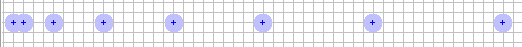
\includegraphics[scale=0.5]{newtons-second-law/puck}
\end{center}
\bigskip


{\bf Answer:}

The puck's velocity is in the direction it is moving which is to the left. Thus, its velocity is in the $-x$ direction. (You can say that its x-component is negative and its y and z components are zero.)

The puck is slowing down as observed by the decreasing distance between marks of the puck. Therefore, its acceleration is in the opposite direction as its velocity, or the $+x$ direction. 

}

\tightframe{

{\bf Question:}

Suppose that the puck in the previous question starts at the left side and moves toward the right side of the image. Marks show the position of the puck at equal time steps. Using our standard definitions of $+x$, $+y$, and $+z$ directions, what is the direction of the velocity and the acceleration of the puck? Is the puck speeding up or slowing down?

{\bf Answer:}

The puck's velocity is in the direction it is moving which is to the right. Thus, its velocity is in the $+x$ direction. (You can say that its x-component is negative and its y and z components are zero.)

The distance between marks of the puck is increasing; therefore, the puck is speeding up. As a result, its acceleration is in the same direction as the velocity (the $+x$ direction).

}

\bigskip
Note that the sign of the acceleration in both of the examples above is positive. It alone does not tell you whether the object will speed up or slow down.

\subsection*{Changing direction with constant speed}

Whenever an object travels along a curved path, it also has an acceleration. Even if it travels with a constant speed, the direction of its velocity changes; therefore, it has a non-zero acceleration.  We can calculate the acceleration in the same way: $\vect{a} = \frac{\Delta \vec{v}}{\Delta t}$. But to visualize the direction of the acceleration, you should find the direction of $\Delta \vec{v}$. Follow this procedure:

\begin{enumerate}
	\item Sketch the vectors $\vec{v}_f$ and $\vec{v}_i$.
	\item Off to the side, sketch $\vec{v}_f$ and $\vec{v}_i$ so that they are drawn tail to tail. Be sure to keep their lengths and directions the same.
	\item Sketch the vector $\Delta \vec{v}$ from the head of $\vec{v}_i$ to the head of $\vec{v}_f$
\end{enumerate}

For example, suppose an object travels in a circle with constant speed, as shown in Figure \ref{newtons-second-law/v-vectors}. Its velocity at two different instances of time is indicated. What is the direction of its acceleration during this time interval?

\scaledimage{newtons-second-law/v-vectors}{Velocity at two locations as it moves along a circle at constant speed.}{0.5}

If you draw the velocity vectors at any locations close together on the circle, you will find that the acceleration vector points toward the center. This is a general observation, \emph{the acceleration of an object that travels in a circle at a constant speed points toward the center of the circle.}

\subsection*{Example}

\tightframe{

{\bf Question:}

A puck bounces off the wall on an air hockey table as shown below. Draw the acceleration vector of the puck during the time interval of the collision.

\bigskip
\begin{center}
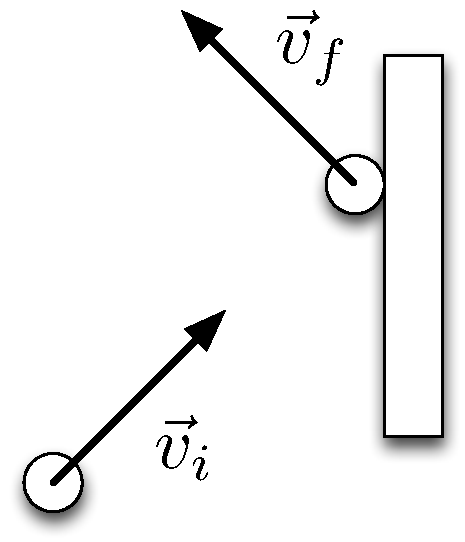
\includegraphics[scale=0.5]{newtons-second-law/wall}
\end{center}
\bigskip


{\bf Answer:}

Sketch the initial and final velocity vectors tail to tail. Then draw $\Delta \vec{v}$ from the head of $\vec{v}_i$ to the head of $\vec{v}_f$. This is the direction of the acceleration. In this case, you can see that it is perpendicular to the wall. The wall must be frictionless.

\bigskip
\begin{center}
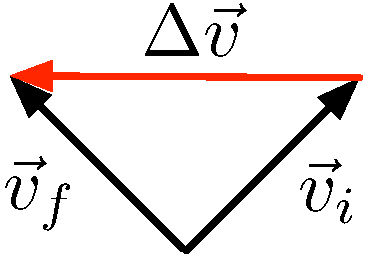
\includegraphics[scale=0.5]{newtons-second-law/collision-acc}
\end{center}
\bigskip

}

\section*{Newton's second law}

The sum of the forces acting on an object is called the \emph{net force}. A net force on an object causes it to accelerate. The object's acceleration is proportional to the net force on the object. The 

\begin{eqnarray*}
	\mbox{acceleration of an object} & = & \frac{\mbox{net force on the object}}{\mbox{mass of the object}} \\
	\vec{a} & = & \frac{\vec{F}_{net}}{m}
\end{eqnarray*}

The acceleration of an object is in the same direction as the net force that acts on it. The net force is what \emph{causes} the acceleration. For a given net force, the larger the mass of the object, the smaller acceleration it will have.

\section*{Predicting the future}

If we know the net force on an object and its velocity, then we can predict its velocity a small time interval later. Since $\vec{a}=(\vec{v}_f-\vec{v}_i)/\Delta t$, then

\begin{eqnarray*}
	\vec{a} & = & \frac{\vec{F}_{net}}{m} \\
	\frac{\vec{v}_f - \vec{v}_i}{\Delta t} & = & \frac{\vec{F}_{net}}{m} \\
	\vec{v}_f & = & \vec{v}_i +  \frac{\vec{F}_{net}}{m}\Delta t
\end{eqnarray*}

This means that Newton's second law can predict the future! It can tell you what the velocity of an object will be after a time interval $\Delta t$. This equation assumes that the net force is constant. If the net force is not constant--that is if the net force is changing during the time interval $\Delta t$-- then we have to use a small time interval.

\begin{eqnarray*}
	\vec{v}_f & \approx & \vec{v}_i +  \frac{\vec{F}_{net}}{m}\Delta t \quad \mbox{for a non-constant force and small time interval}
\end{eqnarray*}

Do not think of $\vec{v}_f$ as ``final'' velocity, but rather think about it as the object's new velocity after a time interval $\Delta t$. In a simulation, we will call this ``updating'' the velocity of the object. Perhaps it is easier to write the equation as:

\begin{eqnarray*}
	\mbox{new velocity} & \approx & \mbox{old velocity} +  \frac{\vec{F}_{net}}{m}\Delta t \qquad \mbox{velocity update equation}
\end{eqnarray*}

Once we know the object's velocity, then we can calculate its new position using the position update equation.

\begin{eqnarray*}
	\mbox{new position} & \approx & \mbox{old position} +   \mbox{new velocity}*\Delta t \qquad \mbox{position update equation}
\end{eqnarray*}

This equation is approximate because the object's velocity is changing due to the force, yet we are assuming for the sake of this calculate that the velocity of the object is constant. This assumption only works for a small time step.

Newton's second law not only explains motion in everyday life, it also allows us to make predictions. Given that we can calculate the net force on an object, we can predict the object's position and velocity at any time in the future by doing these calculations iteratively one small time step after another. 

Wanna know exactly where Jupiter, Mars, and Venus will be on April 6, 2100?  Easy! Just apply Newton's second law and it will tell you.

\section*{Summary of iterative method to predict the future}

\begin{enumerate}
	\item Calculate the net force on the object.
	\item Calculate the new velocity of the object.
	\item Calculate the new position of the object.
	\item Repeat step 1.
\end{enumerate}

\subsection*{Example}

\tightframe{

{\bf Question:}

A 0.4 kg fancart starts at rest at the origin. The air (due to the turning fan) exerts a constant 2 N on the fan in the $+x$ direction. Use the iterative method to calculate the velocity and position of the cart at $t=0.1$ s, $t=0.2$ s, $t=0.3$ s, $t=0.4$ s, and $t=0.5$ s.

{\bf Answer:}

After the first time step, the new velocity of the fancart is

\begin{eqnarray*}
	\mbox{new velocity} & \approx & \mbox{old velocity} +  \frac{\vec{F}_{net}}{m}\Delta t \\
	& = & (0,0,0) + \frac{(2,0,0)\ \newton}{0.4\ \kilo\gram}{0.1\ \second} \\
	& = & (0.5,0,0) \ \meter\per\second
\end{eqnarray*}

The new position of the fancart is (approximately)

\begin{eqnarray*}
	\mbox{new position} & \approx & \mbox{old position} +   \mbox{new velocity}*\Delta t \\
		& = & (0,0,0) + \left((0.5,0,0) \ \meter\per\second\right)(0.1\ \second) \\
	& = & (0.05,0,0) \ \meter
\end{eqnarray*}

and the clock reading will now read $t=0+0.1\ \second=0.1\ \second$.

After the next time step, the new velocity of the fancart is

\begin{eqnarray*}
	\mbox{new velocity} & \approx & \mbox{old velocity} +  \frac{\vec{F}_{net}}{m}\Delta t \\
	& = & (0.5,0,0) \ \meter\per\second + \frac{(2,0,0)\ \newton}{0.4\ \kilo\gram}{0.1\ \second} \\
	& = & (0.5,0,0) \ \meter\per\second + (0.5,0,0) \ \meter\per\second \\
	& = & (1,0,0) \ \meter\per\second
\end{eqnarray*}

The new position of the fancart is

\begin{eqnarray*}
	\mbox{new position} & \approx & \mbox{old position} +   \mbox{new velocity}*\Delta t \\
		& = & (0.05,0,0) \ \meter + \left((1,0,0) \ \meter\per\second\right)(0.1\ \second) \\
	& = & (0.15,0,0) \ \meter
\end{eqnarray*}

and the clock reading is now $t=0.1+0.1\ \second=0.2\ \second$. Continue to calculate the new velocity and new position iteratively for each time step.

\begin{center}
\begin{tabular}{|c|c|c|}
\hline
 t (s) & velocity (m/s) & position (m) \\
\hline
\hline 
  0  & ( 0 , 0 ) & ( 0, 0 )  \\
\hline 
  0.1  & ( 0.5 , 0.0 )  & ( 0.05 , 0.0 )  \\
\hline 
  0.2  & ( 1.0 , 0.0 )  & ( 0.15 , 0.0 )  \\
\hline 
  0.3  & ( 1.5 , 0.0 )  & ( 0.3 , 0.0 )  \\
\hline 
  0.4  & ( 2.0 , 0.0 )  & ( 0.5 , 0.0 )  \\
\hline 
  0.5  & ( 2.5 , 0.0 )  & ( 0.75 , 0.0 )  \\
\hline 
\hline
\end{tabular}
\end{center}

{\bf These are approximate calculations. They have some error and would be more accurate if we used smaller time steps, like 0.01 s.}

}

\pagebreak

\section*{Homework}

\begin{enumerate}
	\item A football bounces off the grass as shown below. 
	
\scaledimage{newtons-second-law/football-bounce}{Velocity before and after a football bounces off the grass.}{1}

Sketch the direction of the acceleration of the football during the collision with the ground.

	\item A ball has an initial position $(-4.5, 0, 0)$ m and an initial velocity $(5.74, 8.19, 0)$ m/s. The mass of the ball is 0.2 kg and the force on the ball is the gravitational force by Earth on the ball, $\vec{F}_{net}=m\vec{g}$, where $\vec{g}=(0,-10,0)$ N/kg at the surface of Earth. The variable $\vec{g}$ is called Earth's \emph{gravitational field strength}.
	\begin{enumerate}
		\item  What is its position and velocity at $t=0.25$ s, $t=0.5$ s, $t=0.75$ s, $t=1.0$ s, $t=1.25$ s, and $t=1.5$ s?
		\item Sketch a coordinate system and sketch the path of the ball by drawing the ball on the coordinate system and connecting the images of the ball with a smooth curve.
	\end{enumerate}

	
\end{enumerate}


\lab{PROGRAM -- Modeling motion of a fancart}

\apparatus

\equip{VPython}
\equip{computer}

\longgoal

In this activity, you will learn how to use a computer to model motion with a constant net force. Specifically, you will model the motion of a fan cart on a track.

\introduction

We are going to model the motion of a cart using the following data.

\bigskip
\noindent
\begin{tabular}{|p{1in}|p{2in}|}
	\hline
	mass of cart & 0.8 kg\\
	\hline
	$\vec{F}_{\mbox{net on cart}}$ & $<0.15,0,0>$ N\\
	\hline
\end{tabular}

\procedure

\begin{enumerate}
	\item Begin with a program that simulates a cart moving with constant velocity on a track.
	
\begin{vpythonblock}
from visual import *

track = box(pos=vector(0,-0.05,0), size=(3.0,0.05,0.1), color=color.white)
cart = box(pos=vector(-1.4,0,0), size=(0.1,0.04,0.05), color=color.green)

cart.m = 0.8
cart.v = vector(1,0,0)

dt = 0.01
t = 0

scene.mouse.getclick()

while cart.pos.x < 1.5 and cart.pos.x >-1.5:
	rate(100)
	cart.pos = cart.pos + cart.v*dt
	t = t+dt
\end{vpythonblock}

	\item Run the program

\smallframe{What does line 12 do? It may help to comment it out and re-run your program to see how it changes things.}

\smallframe{What line updates the position of the cart for each time step?}

\smallframe{What line updates the clock for each time step?}

\smallframe{Is the clock used in any calculations? Is it required for our program?}

\smallframe{What line causes the program to stop if the cart goes off the end of the track?}


We will now apply Newton's second law in order to apply a force to the cart and update its velocity for each time step. There are generally three things that must be done in each iteration of the loop:
	
	\begin{enumerate}
		\item calculate the net force (thought it will be constant in this case)
		\item update the velocity of the cart
		\item update the position of the cart
		\item update the clock (\emph{this is not necessary but is often convenient})
	\end{enumerate}

Your program is already doing the third and fourth items in this list. However, the first two items must be added to your program.

\item Between the \code{rate()} statement and the position update calculation, insert the following two lines of code:

\begin{myvpython}
	Fnet=vector(-0.15,0,0)
	cart.v = cart.v + (Fnet/cart.m)*dt
\end{myvpython}

The first line calculates the net force on the cart (though it is just constant in this case). The second line updates the velocity of the cart in accordance with Newton's second law. After making this change, your \code{while} loop will look like:

\begin{vpythonblock}
while cart.pos.x < 1.5 and cart.pos.x >-1.5:
	rate(100)
	Fnet=vector(-0.15,0,0)
	cart.v = cart.v + (Fnet/cart.m)*dt
	cart.pos = cart.pos + cart.v*dt
	t = t+dt
\end{vpythonblock}

This block of code performs the necessary calculations of net force, velocity, position, and clock reading.

\item Run your program and view the motion.

\smallframe{What is the direction of the net force on the cart? Sketch a side view of the fancart that shows the orientation of the fan.}

Now we will add an arrow object in order to visualize the net force on the cart.  An arrow in VPython is specified by its position (the location of the tail) and its axis (the vector that the arrow represents), as shown in Figure \ref{vpython-fancart/arrow}. The axis contains both magnitude and direction information. The magnitude of the axis is the arrow's length and the unit vector of the axis is the arrow's direction. The components of the axis are simply the components of the vector that the arrow represents.

\scaledimage{vpython-fancart/arrow}{A arrow in VPython.}{0.75}

\item Near the top of your program after creating the track and cart, add the following two lines to define a scale and to create an arrow that has the same components $(-0.15,0,0)$ as the net force on the cart.

\begin{myvpython}
scale=1.0
forcearrow = arrow(pos=cart.pos, axis=scale*vector(-0.15,0,0), color=color.yellow)
\end{myvpython}

\item Run your program.

\item Increase the scale and re-run your program.

\smallframe{What does changing the scale do? Why do we want to use this variable and adjust it?}

\smallframe{Why does the arrow not move with the cart?}

\item We want to make the arrow move with the cart. Thus, in our loop we need to update the position of the arrow after we update the position of the cart. Also, in some situations, the force changes, so in general it's a good idea to update the arrow's axis as well. At the bottom of your \code{while} loop, after you've updated the clock, add the following lines in order to update the position of the arrow and the axis of the arrow.

\begin{myvpython}
	forcearrow.pos=cart.pos
	forcearrow.axis=scale*Fnet
\end{myvpython}

\item Run your program.

\end{enumerate}

\report

\begin{description}

\item[C]  Complete the experiment and report your answers for the following questions.

\begin{enumerate}
	 \item Does the simulation behave like a real fancart?
	\item Though the velocity of the cart changes as it moves, does the force change or is the force constant?
	\item Does the acceleration of the cart change or is the car's acceleration constant?
	\item When the cart passes $x=0$, turn off the fan (i.e. set the net force on the cart to zero). Describe the resulting motion of the cart. What is the velocity of the cart after the fan turns off?
\end{enumerate}

\item[B] Do all parts for {\bf C} do the following.

\begin{enumerate}
 \item Add a second arrow that represents the velocity of the cart. Update its position and its axis. Give it an appropriate scale.
\end{enumerate}

\item[A] Do all parts for {\bf C} and {\bf B} and do the following.

\begin{enumerate}
 \item Add keyboard interactions that allow the user to make the force zero (i.e. turn off the fan), turn on a constant force to the right, or turn on a constant force to the left. In all of these cases, the arrow should indicate the state of the fan.
 \item Check that your code results in correct motion. Compare to how a real fan cart would behave. Describe what you did to test your code, and describe what observations you made that convince you that it works correctly. Your description of the motion of the cart should be accompanied by pictures with force and velocity arrows.
\end{enumerate}
\end{description}
\lab{GAME -- Lunar Lander}

\apparatus
\equip{Computer}
\equip{GlowScript -- www.glowscript.org}

\longgoal

The purpose of this activity is to create a Lunar Lander game where you have to land the lunar module on the moon with as small a speed as possible and as quickly as possible. If the speed is too high, it crashes. If it takes you forever, then you run out of fuel.

\procedure

In the previous simulation that you wrote, you learned how to model the motion of an object on which the net force is constant. In that case, the object was a fancart. You learned how to apply Newton's second law to update the velocity of an object given the net force on the object. Once you can do this, you can model the motion of \emph{any} object. As a reminder, the important steps in each iteration of the loop are to:

	\begin{enumerate}
		\item calculate the net force (although in some cases it is constant)
		\item update the velocity of the cart
		\item update the position of the cart
		\item update the clock (\emph{this is not necessary but is often convenient}).
	\end{enumerate}
	
The net force may not be constant. For example, you can check for keyboard interactions and turn a force on or off, or the net force might depend on direction of motion (such as friction) or speed (such as drag) or position (such as gravitational force of a star on a planet). This is why you have to calculate the net force during each iteration of the loop.

To develop a lunar lander game, we are going to begin with a bouncing ball that makes an elastic collision with the floor. 

\begin{enumerate}

\subsection*{A bouncing ball}

\item Here is a template for a program that simulates a bouncing ball. {\bf However, a few essential lines are missing.} Type the template below but do not run the code (since lines are missing). It is fine if the first line references a more recent version of GlowScript.

\begin{vpythonblock}
GlowScript 2.1 VPython

scene.range=20

ground = box(pos=vector(0,-10.05,0), size=vector(40.0,1,1), color=color.white)
ball = sphere(pos=vector(0,9,0), radius=2, color=color.yellow)

ball.m = 1
ball.v = vector(0,0,0)
g=vector(0,-10,0)

dt = 0.01
t = 0

scale=1
FgravArrow = arrow(pos=ball.pos, axis=scale*ball.m*g, color=color.red)

scene.waitfor("click")

while 1:
    rate(100)
#    Fgrav=
#    Fnet=
#    ball.v = 
#    ball.pos = 
    if(ball.pos.y-ball.radius < ground.pos.y+ground.height/2):
            ball.v=-ball.v
    t = t+dt
    FgravArrow.pos=ball.pos
    FgravArrow.axis=scale*Fgrav
\end{vpythonblock}

\smallframe{Line 10 defines a vector $\vec{g}$. What is this vector called? What is its direction, and what is its magnitude?}

\item Line 22 should compute the gravitational force on the ball. Fill in this line using the variables for the mass of the ball and Earth's gravitational field.

\item Line 23 is the net force on the ball. This is computed by summing all forces on the ball. But the only force on the ball in this case is the gravitational force. Fill in line 23 with the variable representing the gravitational force on the ball.

\item Line 24 updates the velocity of the ball and line 25 updates the position. Fill in each of these lines with the appropriate calculation for updating the velocity and position of the ball. Refer to the previous chapter on the fancart if you forget how to do this.

\item Run your program and make sure it shows a bouncing ball.

\smallframe{What is the purpose of lines 26 and 27?}

\smallframe{If line 26 was changed to \code{if(ball.pos.y < ground.pos.y):}, what would occur and why is this worse than the original version of line 26? (You should comment out line 26 and type this new code in order to check your answer.)}

\smallframe{Is the gravitational force on the ball constant or does it change? Explain your answer.}

\item The Moon has a gravitational field that is 1/6 that of Earth. Change $\vec{g}$ to model the motion of a bouncing ball on the Moon and re-run your program.

\smallframe{What is the primary difference in the motion of a ball dropped on the Moon and a ball dropped from the same height on Earth? In other words, if you were to see an animation of each ball, side by side, how would you know which animation is of the ball on the Moon?}

\subsection*{Moon Lander}

We will now model the motion of a lunar module that is landing on the moon. 

\scaledimage{game-lunar-lander/apollo}{Apollo 16 LM \emph{Orion}}{1}

\item Start a new program and type the following code into GlowScript.

\begin{myvpython}
GlowScript 2.1 VPython

scene.range=20

ground = box(pos=vector(0,-10.05,0), size=vector(40.0,1,1), color=color.white)
spaceship = box(pos=vector(0,8,0), size=vector(2,5,2), color=color.yellow)

spaceship.m = 1
spaceship.v = vector(0,0,0)
g=1/6*vector(0,-10,0)

dt = 0.01
t = 0

scale=5.0
FgravArrow = arrow(pos=spaceship.pos, axis=scale*spaceship.m*g, color=color.red)

while 1:
    rate(100)
#    Fgrav=
#    Fnet=
#    spaceship.v = 
#    spaceship.pos = 
    if(spaceship.pos.y-spaceship.height/2<ground.pos.y+ground.height/2):
            print("spaceship has landed")
            break
    t = t+dt
    FgravArrow.pos=spaceship.pos
    FgravArrow.axis=scale*Fgrav
\end{myvpython}

\item Fill in lines 20-23 with the appropriate expressions.

\item We are now going to add a force of thrust due to rocket engines. Before the \code{while} loop, define a thrust force.

\begin{myvpython}
Fthrust=vector(0,4,0)
\end{myvpython}

\item After defining the thrust vector, create another arrow that will represent the thrust force. Call it \code{FthrustArrow} as shown.

\begin{myvpython}
FthrustArrow = arrow(pos=spaceship.pos, axis=scale*Fthrust, color=color.cyan)
\end{myvpython}

\item In the while loop, change the net force so that it is the sum of the gravitational force and the thrust of the rocket engine.

\begin{myvpython}
        Fnet=Fgrav+Fthrust
\end{myvpython}

\item Also, in the while loop, update the thrust arrow's position and axis.

\begin{myvpython}
        FthrustArrow.pos=spaceship.pos
        FthrustArrow.axis=scale*Fthrust
\end{myvpython}

\item Run your program and verify that the motion of the spaceship is what we expect from Newton's second law. 

\smallframe{Change the thrust to 10/6 N (in the $+y$ direction. Describe the motion. Is this consistent with Newton's second law?}

Let's use the keyboard to turn on and off the engine. In this case, ``on'' means that the vertical thrust is $(0,4,0)$ and ``off'' means that the thrust is zero, $(0,0,0)$. 

\item Create a new program. Copy and paste your last program into this new file, and set the value of \code{Fthrust} to zero, $(0,0,0)$. Run your program and verify that the lunar module accelerates downward and stops when reaching the Moon's surface. (Make sure that $g=(0,-10/6,0)$ N/kg.

\item Near the top of your program at approximately line 2, add the following function.

\begin{myvpython}
##add keyboard control
def process(event):
    global Fthrust
    if event.type=='keydown':
        k = event.which
        if k == 38: #up arrow turns on the vertical thruster
            Fthrust=vector(0,4,0)
    elif event.type=='keyup': #releasing the key turns off the thruster
        Fthrust=vector(0,0,0)

    FthrustArrow.axis=scale*Fthrust
        
scene.bind('keydown keyup', process) 
\end{myvpython}

\smallframe{What key is used to turn on the thruster? What causes the thruster to turn off?}
        
\item Run your program and verify that it works. Use the up arrow key to control the thruster. Land the lunar module as gently as possible on the Moon's surface.

\end{enumerate}

\pagebreak

\analysis

\begin{description}

\item[C] Complete this exercise and do the following.

\begin{enumerate}
	\item Print the speed of the spaceship and the clock reading when it lands.
\end{enumerate}


\item[B] Do everything for {\bf C} and the following.

\begin{enumerate}
	\item If the speed of the spaceship is greater than a minimum requirement (like 1 m/s), print ``You lose.''
	\item If the speed of the spaceship is less than this minimum, print ``You win.''
\end{enumerate}

\item[A] Do everything for {\bf B} with the following modifications and additions.

\begin{enumerate}
	\item Create an engine that fires in the $+x$ direction (the engine is on the left so the arrow points to the right) when the right arrow key is pressed.
	\item Create an engine that fires in the $-x$ direction (the engine is on the right so the arrow points to the left) when the left arrow key is pressed.
	\item Place a target on the ground.
	\item Check that the lunar module lands on the target.
	\item Check that the x-velocity is very small (perhaps less than 1 m/s for example) when the spaceship hits the target and print ``You win'' if and only if the spaceship has a very small x-velocity.
	\item Since you don't want to waste fuel, assign points based on the time elapsed and cause the player to lose if the clock reading exceeds some amount. If you want, you can create a timer that starts at some value like 20 s and counts down to zero.
\end{enumerate}




\end{description}


\lab{LAB: Video Analysis of Projectile Motion}

\apparatus

%public web site
%\equip{Tracker software (free; download from \href{http://www.cabrillo.edu/~dbrown/tracker/}{http://www.cabrillo.edu/$\sim$dbrown/tracker/})}
%\equip{video: \code{basketball.mov} from \href{http://physics.highpoint.edu/~atitus/videos/}{http://physics.highpoint.edu/$\sim$atitus/videos/}}

%our course web site
\equip{Tracker software (free; download from \href{http://www.cabrillo.edu/~dbrown/tracker/}{http://www.cabrillo.edu/$\sim$dbrown/tracker/})}
\equip{video: \code{basketball.mov} from our course web site.}

\longgoal

In this experiment, you will measure and graph the x-position, y-position, x-velocity, and y-velocity of a projectile, in this case a basketball as it moves freely through air with negligible air resistance. 

\introduction

Suppose a projectile moves along a parabolic path. Fig. \ref{video-projectile-motion/projectile-with-axes} shows an object at intervals of 1/30 s between the first image A and the last image I.

\scaledimage{video-projectile-motion/projectile-with-axes}{Position of a projectile at equal time intervals of 1/30 s.}{0.8}

\tightframe{Suppose that we define $t=0$ to occur at the first position of the object. In Fig. \ref{video-projectile-motion/projectile-with-axes}, label the time $t$ for each subsequent position of the object.}

\tightframe{Draw a vertical line at the location of each image. Where each vertical line intersects the x-axis, sketch a circle on the x-axis at the x-coordinate of each image in Fig. \ref{video-projectile-motion/projectile-with-axes}. An example is shown in Fig. \ref{video-projectile-motion/projectile-x}.}

\scaledimage{video-projectile-motion/projectile-x}{x-positions of the projectile.}{0.8}

\smallframe{By examining the x-coordinate of the object, is the x-motion characterized by uniform motion (i.e. zero net force) or constant acceleration (i.e. constant net force)? Give a reason for your answer.}

\smallframe{If you were to graph $x$ vs. $t$, what would it look like? Draw a sketch.}

\smallframe{In Fig. \ref{video-projectile-motion/projectile-with-axes}, mark the y-position of the projectile by drawing horizontal lines from the object to the y-axis and drawing a circle where this line intersects the y-axis. Is the y-motion characterized by uniform motion (zero net force) or constant acceleration (constant net force)? Give a reason for your answer.}

\smallframe{If you were to graph $y$ vs. $t$, what would it look like? Draw a sketch.}


\procedure

\begin{enumerate}

	\item Download the file \texttt{basketball.mov} by right-clicking on the link and choosing {\bf Save As...} to save it to your desktop.
	\item Open the \file{Tracker} software on your computer.
	\item Use the menu \menu{Video$\to$Import...} to import your video, as shown in Figure \ref{video-projectile-motion/video-import}.

\scaledimage{video-projectile-motion/video-import}{Video$\to$Import menu}{0.5}

	\item Play the video and watch the motion of the basketball. 
	
	\smallframe{What is the shape of its path?}

	\smallframe{After the ball leaves the player's hand, what interacts with the ball and in what direction does it exert a force on the ball?}

	\item Use the video control bar to advance the video to the first frame after the ball leaves the player's hand. We are only studying the motion of the ball while it is in the air, not while it is in his hand. Use the Video Settings to make this the first frame of the video. Also set the last frame of the video to be the frame when the ball hits the floor.

	\item You now need to define the origin of the coordinate system. In the toolbar, click the \menu{Axes} icon shown in Fig. \ref{video-projectile-motion/coord-icon} to show the axes of the coordinate system.
	
	\image{video-projectile-motion/coord-icon}{Icon used to set the coordinate system axes.}

	\item Click and drag on the video to place the origin of the coordinate system at the location where you would like to define (0,0). For consistency with your classmates, place the origin on the floor at the center of the player's feet.
		
%	\scaledimage{video-projectile-motion/coord-sys}{Click and drag to set the origin of the coordinate system}{0.3}
		
	\item We will use the 2-m long stick that is along the base of the wall to set the scale for the video.  In the toolbar, click on the \menu{Tape Measure} icon shown in Figure \ref{video-projectile-motion/ruler} to set the scale for the video.
		
	\scaledimage{video-projectile-motion/ruler}{Icon used to set the scale.}{1}

	\item A blue double-sided arrow will appear. Move the left end of the arrow to the left end of the stick, and move the right end of the arrow to the right end of the stick. Double-click the number that is in the center of the arrow, and enter the length of the stick (2.0). (Our units are meters, but Tracker does not use units. You must remember that the number 2.0 is given in meters.) The scale will appear as shown in Figure \ref{video-projectile-motion/set-scale}.

	\scaledimage{video-projectile-motion/set-scale}{Enter the length of the stick, 2.0 m.}{0.3}

	\item Click the tape measure icon again to hide the blue scale from the video.
	
	\item To mark the position of the basketball in each frame, first click on the \button{Create} button and select \menu{Point Mass}. Then, {\bf mass A} will be created, and a new $x$ vs. $t$ graph will appear in a different pane. You will now be able to mark the position of the ball which will be referred to as {\bf mass A}.

	\item Now, to mark the position of the basketball, hold down the shift key and click on the ball. (This is called a shift-click). The video will advance one frame. Continue to shift-click on the ball until you have marked the location of the ball in all frames of the video.
	
	Keep in mind that you only want to analyze frames where the ball is in the air. Therefore, you should have skipped the first few frames when it is in the player's hand, and you should stop marking the position of the ball just before it hits the floor.
	
		\item It's possible that only a few of the marks are shown in the video pane. To display all of the marks or a few of the marks or none of the marks, use the \menu{Set Trail Length} icon shown in Figure \ref{video-projectile-motion/set-trail}. Clicking this icon continuously will cycle through no trail, short trail, and full trail which will show you no marks, a few marks, or all marks. 

	\scaledimage{video-projectile-motion/set-trail}{The Set Trail icon is used to vary the number of marks shown.}{1}

	A picture of the basketball with marks is shown in Figure \ref{video-projectile-motion/trail}.
	
	\scaledimage{video-projectile-motion/trail}{Marks showing the motion of the basketball.}{0.3}	

\end{enumerate}

\analysis

\begin{enumerate}
	\item View the $x$ vs. $t$ graph. You can click and drag the border of the video pane to make it smaller so that you can focus on the graph.
	
	\item Play the video. (You can hide the marks if you wish by clicking the \menu{Show or hide positions} icon, and you can show the path by clicking the \menu{Show or hide paths} icon. Both of these icons are in the toolbar.) Note how the graph and video are synced. The data point corresponding to the given video frame is shown in the graph using a filled rectangle.
	
	Also, when you click on a data point on the graph, the video moves to the corresponding frame.
		
	\tinyframe{Describe in words the type of function that describes this graph of x vs. t? (i.e. linear, quadratic, square root, sinusoidal, etc.)}
	
	\smallframe{According to the $x$ vs. $t$ graph, is the x-velocity constant, increasing, or decreasing? Explain your answer.}
	
	\smallframe{Based on this graph, what is the x-component of the net force on the ball while it is in the air, $F_{net,x}$?}
					
	\item  Right-click on the graph (or ctrl-click for Mac users) and select \menu{Analyze...}. In the resulting window, check the checkbox for \menu{Fit}, and additional input boxes will appear, as shown in Figure \ref{video-projectile-motion/x-t-fit}. Select the Fit Name ``Line,'' and the equation will be $x=a*t+b$ where $a$ and $b$ are coefficients (or parameters) of the curve fit. Check the checkbox for \menu{Autofit} and the best-fit curve will appear in the graph.
	
	\scaledimage{video-projectile-motion/x-t-fit}{The Data Tool for finding the best-fit curve for the data.}{0.3}
	
	
	\item  Find the best-fit curve for the graph. Be sure to select the linear fit.
		
	\smallframe{Neatly sketch the graph, including axes and labels, below.}
	
	\smallframe{Record the function and the values of the constants for your curve fit. Write the function for x(t), with the appropriate constants (also called fit parameters).}
		
	\smallframe{What do you expect the x-velocity vs. time graph to look like? Sketch your prediction below.}
		
	\item Close the Data Tool window and return to the main Tracker window. Click on the label of the vertical axis on the graph and select \menu{vx}.
		
	\smallframe{What function describes this graph of $v_x$ vs. $t$? (i.e. linear, quadratic, square root, sinusoidal, etc.)}
	
	\item Right-click the graph and select \menu{Analyze} to analyze the $v_x$ vs. $t$ graph. You may notice that the data for both $x$ and $v_x$ are displayed on the same graph. If this occurs, uncheck the checkboxes for $x$ in the upper right corner of the window.
			
	\smallframe{Neatly sketch the graph of $v_x$ vs. $t$, including axes and labels, below.}
	
	\smallframe{Use this graph and data to determine $v_x$. Describe in detail how you determined $v_x$. }
	
	\item Close this window and return to the main window. Change the label on the vertical axis to $y$ vs. $t$ and examine this graph.

	\smallframe{According to the $y$ vs. $t$ graph, during what time interval is the magnitude of the y-velocity decreasing? During what time interval is the magnitude of the y-velocity increasing? At what time is the y-velocity zero?}

	\item Change the label on the vertical axis to $v_y$ vs. t and examine this graph. 

	\smallframe{Based on this graph, is the y-component of the net force on the ball, $F_{net,y}$, zero or constant (non-zero)? If it is constant (and non-zero), explain your reasoning and say whether the net force on the ball is in the +y or -y direction.}
	
	\item Right-click the graph and select \menu{Analyze} to analyze the $v_y$ vs. $t$ graph. Fit a curve to the data and record the best-fit function, including the fit parameters. An example is shown in Figure \ref{video-projectile-motion/vy-t-fit}.
	
	\smallframe{\ }

	\scaledimage{video-projectile-motion/vy-t-fit}{The Data Tool for finding the best-fit curve for the $v_y$ vs. t data.}{0.3}

	
	\smallframe{What is the y-velocity $v_y$ of the ball at the moment it leaves the player's hand?}
	
	\smallframe{What is the ball's y-acceleration, $a_y$?  Since the mass of a basketball is about 0.62 kg, also calculate the y-component of the net force on the basketball, $F_{net,y}$.}
		
\end{enumerate}

\report

\begin{description}

\item[C]  Complete the experiment and report your answers to the following questions.

\begin{enumerate}
	 \item What is the x-component of the net force on the ball? (Explain your reasoning or show your calculation.)
	 \item What is the x-velocity of the basketball as determined by the $x(t)$ graph? (Explain your reasoning.)
	 \item What is the y-acceleration of the ball as determined by the $v_y(t)$ graph? (Explain your reasoning.)
	 \item What is the y-component of the net force on the ball? (Explain your reasoning or show your calculation.)
\end{enumerate}

\item[B] Do all parts for {\bf C} and answer the following questions.

\begin{enumerate}
	\item What is the velocity of the ball at the instant it leaves the player's hand ($t=0$)? Write it as a vector and sketch it.
	\item What is the position (x and y components) of the basketball at the first instant that it leaves the player's hand ($t=0$)?
	\item At what clock reading $t$ is the ball at its peak and explain how you can get this independently by looking at the $y(t)$ graph and by looking at the $v_y(t)$ graph.
	\item What is the velocity of the ball when it is at its peak? Express your answer as a vector.
\end{enumerate}

\item[A] Do all parts for {\bf B} and answer the following questions.

\begin{enumerate}
	\item Starting with Newton's second law and the initial position and velocity of the ball, calculate the position and velocity of the ball at 0.05 s time steps. What is its position and velocity at $t=0.25\ \second$?
	\item Compare your theoretical calculation in the previous question with the actual data for position and velocity at or near $t = 0.25$ s. How do they compare? (Note that the iterative calculation is approximate and is only accurate for very small time steps. There may be some discrepancy since we used a larger time step.)
	\item Go back to your iterative calculation and continue until the ball reaches its maximum height (i.e. $v_y\approx0$). What is the approximate clock reading $t$ when the ball reaches its peak? Compare your theoretical calculation with what you measured. (Again there may be some discrepancy due to the fact that the iterative method is an approximation.)
\end{enumerate}
\end{description}

%Answer Key

%[C]
%
%(a) zero; because the x-velocity is constant
%(b) 3.07 m/s
%(c) -9.8 m/s/s
%(d) Fnety = m*ay and is in the -y direction
%
%[B] 
%
%(a) v = (3.07, 4.52) m/s.  The initial y-velocity is the intercept on the vy vs. t graph
%(b) r = (0.52, 2.66) m. This is the first data point for (x,y)
%(c) from y(t), it is t=0.47 s where y is a max; from vy(t), it is t=0.47, where vy=0.
%(d) v = (3.07,0) m/s
%
%[A]
%
%(a) at t=0.25, r=(1.2875, 3.4225, 0) m, and v= (3.07, 2.07, 0) m/s
%(b) at t=0.25, r ~ (1.3,3.5) m and v ~ (3.05, 2.0) m/s.  To one decimal place, these values are within 0.1 of the measured values.
%(c) vy=0 between t=0.5 and t=0.55 s. The peak occurs at 0.47 s according to the data. The prediction and the actual time are off by about one time step.


\lab{LAB: Angry Birds}

\apparatus

\equip{Tracker software (free; download from \href{http://www.cabrillo.edu/~dbrown/tracker/}{http://www.cabrillo.edu/$\sim$dbrown/tracker/})}
\equip{video: \code{Angry\_Birds.mp4} from our course web site.}
\equip{Tracker file: \code{Angry\_Birds\_projectile.trk} from our course web site.}

\longgoal

In this experiment, you will measure the motion of a bird in Angry Birds and will assume $g=10\ \meter\per\second^2$ in order to calibrate distance in the video. You will also see if the resulting motion of the bird is consistent with projectile motion. In other words, has the programmer of Angry Birds used correct physics in the game?

\introduction

In the game Angry Birds, birds are launched with a slingshot. Is their motion described by ideal projectile motion? If so, what is the acceleration of a bird and can we use its acceleration to figure out the length of a bird? 

When we do video analysis, we typically use an object of known length in the video to calibrate the video and determine how many pixels is 1 m. In the case of Angry Birds, instead of scaling the video with a known object on the screen, we can scale the video by the acceleration due to gravity, assuming the Angry Birds world is Earth. That is, we can assume that $a_y=-g=-10\ \meter\per\second^2$, then calculate the scaling factor, and use the scaling factor determine the length of objects in the video in units of meters.

\procedure

\begin{enumerate}
	\item Download the file \file{Angry\_Birds.mp4} from our course web site.
	\item Download the file \file{Angry\_Birds\_projectile.trk} from our course web site.
	\item The \file{.trk} file is a partially marked Tracker file. Open the Tracker software. Go to \menu{File$\to$Open File...} and select the file \file{Angry\_Birds\_projectile.trk}. It should load the video or ask you where it is located.
	\item Play the video and notice that the ``camera'' both moves (i.e. pans) and zooms. This makes analyzing the video more difficult than what you've encountered before.

In order to track the bird, we will need a fixed origin (the sling slot), and since the origin goes off screen, we need an offset point (the distance from the sling shot to a blade of grass that shows up for most of the trajectory of the bird).

	We also need a set length since the movie zooms in and out. It turns out that the height to the fork of the slingshot is the same as the height of the first pedestal the pig sits on. We will define the height of the fork of the slingshot as ``1'' \emph{slingshot} in the Tracker file. So, even as the image zooms and pans, the length of the slingshot and the pig's pedestal is always ``1'' and the location of the origin is set. DO NOT adjust the ``Coordinate Offset'' or the ``Calibration Stick'' or the data will no longer account for the panning and zooming of the camera.
	
	\tightframe{Remember that our unit of distance in the video will be \emph{slingshots} because this is the height of the slingshot from its base to the fork. Thus, all distances are in $slingshots$ and all velocities are in $slingshots/s$.}
	
	\smallframe{The Tracker file already has the position of the angry bird marked.  The track of the marked points is not a parabola on the video. Why not?}
	
	\item Verify that the graph plots $y(x)$. If necessary, click on the vertical axis variable and change it to $y$, and click on the horizontal axis variable and change it to $x$. This will display the calculated path of the bird after accounting for the zooming and panning of the camera.
	
	\smallframe{What is the calculated path of the bird? Describe it in words and sketch it.}
	
	\smallframe{Explain why some points are missing.}
	
	\smallframe{If the bird follows correct physics, what should a graph of x(t) look like? Sketch it below.}
	
	\item Change the vertical axis variable to $x$ and change the horizontal axis variable to $t$. 
	
	\smallframe{Explain why the plot of x(t) is a straight line.}
	
	\smallframe{What is the best-fit function for $x(t)$?}
	
	\smallframe{From this best-fit function, what is $v_x$ in units of slingshots/s?}

	\item Change the vertical axis variable to $y$ and change the horizontal axis variable to $t$. Notice that it is parabolic. At first the slope decreases, showing that the bird slows down as it rises. Then the slope increases, showing that the bird speeds up as it falls.
	
	\item Change the vertical axis variable to $v_y$. Due to measurement error there is variation in the data; however, it generally appears linear. Do a linear fit.
	
	\smallframe{What is the best-fit function for the $v_y(t)$ graph?}
	
	\smallframe{From the best-fit function, what is the y-acceleration in units of slingshots/s$^2$?}
	
	\smallframe{What is the initial y-velocity in slingshots/s?}
	
	\smallframe{By comparing the measured y-acceleration in slingshots/s$^2$ to free-acceleration on Earth of $-10$ m/s$^2$, how many slingshots are in 10 m?}
		
	\smallframe{How many meters is 1 slingshot?}
	
	\smallframe{Use the tape measure to measure the radius of the bird in units of slingshots. Convert this to meters. Is this a realistic size for a bird?}
	
	\smallframe{Convert the x-velocity and initial y-velocity to m/s. What is the initial velocity vector in m/s?  What is the initial speed of the bird in m/s?}
	
\end{enumerate}

\report

\begin{description}

\item[C]  Complete the experiment and report your answers to the following questions.

\begin{enumerate}
	 \item What is the x-velocity of the bird in units of slingshots/s?
	 \item Is the x-velocity of the bird increasing, decreasing, or constant?
	 \item What is the x-acceleration?
	 \item What is the initial y-velocity of the bird in units of slingshots/s?
	 \item Is the y-velocity of the bird increasing, decreasing, or constant?
	 \item What is the y-acceleration of the bird in units of slingshots/s$^2$?
\end{enumerate}

\item[B] Do all parts for {\bf C} and answer the following questions.

\begin{enumerate}
	\item Generally, the videos that we analyze have an object of known distance. In this case, what is the ``known'' quantity that we used to determine distance in meters in the video?
	\item How many meters are in 1 slingshot?
	\item What is the radius of the bird in units of meters?
	\item What is the initial velocity vector of the bird in m/s?
	\item What is the initial speed of the bird in m/s?
\end{enumerate}

\item[A] Do all parts for {\bf B} and answer the following questions.

\begin{enumerate}
	\item Suppose that you analyze a video screen capture of a tank wars game. You use the length of the tank as the unit ``1 tank'' and find that the free-fall y-acceleration in the world of the game is $-2.5\ tanks/s^2$. How many meters long is the tank?
	\item You analyze a bullet in the tank wars game. Its x(t) graph with x in meters is shown below. What is the x-velocity of the projectile?
	
\scaledimage{video-angry-birds/x-t-graph}{x(t) for a projectile.}{0.8}

	\item What is the x-acceleration of the projectile?
	
	\item The projectile's $v_y(t)$ graph is shown below. What is the initial y-velocity of the projectile?

\scaledimage{video-angry-birds/vy-t-graph}{$v_y(t)$ for a projectile.}{0.8}
	
	\item What is the y-acceleration of the projectile?
	
	\item At what time (i.e. clock reading) did the projectile reach its peak?
	
	\item What is the initial velocity vector of the projectile?
	
	\item What is the initial launch speed of the projectile?
	
\end{enumerate}
\end{description}

% Answers

%[C]
%
%(a) 4.64 slingshots/s
%(b) vx is constant
%(c) 0
%(d) 6.97 slingshots/s
%(e) vy decreases
%(f) ay = -3.8 slingshots/s/s
%
%[B]
%
%(a) free-fall acceleration due to gravity on earth (-10 m/s/s)
%(b) 2.6 m in 1 slingshot
%(c) 0.47 m
%(d) v=(12,18) m/s
%(e) |v| = 22 m/s
%
%[A]
%
%(a) 3.9 m
%(b) 4 m/s
%(c) 0
%(d) vy=10 m/s
%(e) ay=-2.5 m/s/s
%(f)  t = 4 s
%(g) v=(4,10) m/s
%(h) |v| = 11 m/s

\lab{GAME -- Tank Wars}

\apparatus
\equip{Computer}
\equip{VPython -- www.vpython.org}

\longgoal

The purpose of this activity is to create a Tank Wars game where you will move a tank and adjust the launch angle and launch speed to hit a target.

\procedure

\begin{enumerate}
        
\item Download the program \file{tank-wars-template.py} from our course web site. For your reference, the program is printed below.

\begin{vpythonblock}
from visual import *

def rad(degrees): #converts an angle in degrees to an angle in radians
    radians=degrees*pi/180
    return radians

scene.range=20
scene.width=800
scene.height=800

#create objects
ground = box(pos=vector(0,-15,0), size=(40.0,1,2), color=color.green)
tank = box(pos=vector(-18,-13,0), size=(2,2,2), color=color.yellow)
turret = cylinder(pos=tank.pos, axis=(0,0,0), radius=0.5, color=tank.color)
turret.pos.y=turret.pos.y+tank.height/2
angleBar = cylinder(pos=vector(-18,-19,0), axis=(1,0,0), radius=1, color=color.magenta)
speedBar = cylinder(pos=vector(5,-19,0), axis=(1,0,0), radius=1, color=color.cyan)

#turret
theta=rad(45)
dtheta=rad(1)
L=3
turret.axis=L*vector(cos(theta),sin(theta),0)

#bullets
bulletsList=[]
m=1
muzzlespeed=15
dspeed=1

#Bar
angleBar.axis=(5*theta)*vector(1,0,0)
speedBar.axis=(muzzlespeed/2+0.5)*vector(1,0,0)

#motion
g=vector(0,-10,0)
dt = 0.01
t = 0

while 1:
    scene.mouse.getclick()
    while 1:
        rate(100)
        if scene.kb.keys:
            k = scene.kb.getkey()
            if k == "up":
                theta=theta+dtheta
                turret.axis=L*vector(cos(theta),sin(theta),0)
                angleBar.axis=(5*theta)*vector(1,0,0)
            elif k == "down":
                theta=theta-dtheta
                turret.axis=L*vector(cos(theta),sin(theta),0)
                angleBar.axis=(5*theta)*vector(1,0,0)
            elif k == "left":
                muzzlespeed=muzzlespeed-dspeed
                speedBar.axis=(muzzlespeed/2+0.5)*vector(1,0,0)
            elif k == "right":
                muzzlespeed=muzzlespeed+dspeed
                speedBar.axis=(muzzlespeed/2+0.5)*vector(1,0,0)
            elif k==" ":
                bullet=sphere(pos=turret.pos+turret.axis, radius=0.5, color=color.white)
                bullet.v=muzzlespeed*vector(cos(theta),sin(theta),0)
                bulletsList.append(bullet)
            elif k=="Q":
                break

        if muzzlespeed>20:
            muzzlespeed=20
        if muzzlespeed<1:
            muzzlespeed=1
        if theta>rad(90):
            theta=rad(90)
        if theta<0:
            theta=0

        for thisbullet in bulletsList:
            if(thisbullet.pos.y<ground.y+ground.height/2):
                thisbullet.Fnet=vector(0,0,0)
                thisbullet.v=vector(0,0,0)
            else:
                thisbullet.Fnet=m*g
#            thisbullet.v=
#            thisbullet.pos=

        t=t+dt

\end{vpythonblock}

\item Read the program above and answer the following questions.

\smallframe{What should lines 82 and 83 be in order to correctly update a bullet's velocity and position for each time step?}

\smallframe{Is the world in this simulation Earth?  Cite a particular line number in the code in order to support your answer.}

\smallframe{What does the \code{rad()} function do?}

\smallframe{What does the variable $L$ tell you?}

\smallframe{What is the variable name for the initial speed of the bullet? How much does the launch speed of the bullet change when you press the right or left arrow key?}

\smallframe{What is the variable name for the angle the bullet is launched at? How much does the angle change when you press the right or left arrow key and is the unit radians or degrees?}


\smallframe{After a bullet hits the ground, what is the net force on the bullet and what is its velocity? Cite the particular line numbers that support your answer.}

\smallframe{What key strokes are used to change the launch angle?}

\smallframe{What keystrokes are used to change the launch speed?}

\smallframe{What is the maximum and minimum launch speeds allowed? Which line numbers tell you this?}

\smallframe{What is the maximum and minimum angles allowed? Which line numbers tell you this?}

	\item Edit lines 82 and 83 so that they use correct physics to update the velocity and position of each bullet and run the program.
	
The reason that there are nested \code{while} loops is that you are going to create a target, and after a bullet hits the target, you may want to pause the game, reset certain variables, add a barrier, count a score, etc. The inner while loop handles the animation and the outer while loop is where you'll do other things after the target is hit. At this point, the outer loop only runs one iteration and only pauses the program, waiting for a mouse click.

We are now going to add a few features to the game.

\subsection*{Creating a Target}

	\item Create a target that is a box named \code{target} that is the size of the tank and place it somewhere else on the terrain. Run your program to see the target.
	
We will need to check for collisions between a bullet and the target. It is convenient to create a function that does the math to see if the bullet (sphere) and target (box) overlap. If they do overlap, it returns \code{True}. If they do not overlap, the it returns \code{False}.

	\item At the top of your program near where the \code{rad()} function is defined, add the following function. You do not have to type the commented lines. You will need to double check your typing to make sure you do not have any typos. The condition of the \code{if} statement is rather long, so check it for accuracy.
	
\begin{myvpython}
#determines whether a sphere and box intersect or not
#returns boolean
def collisionSphereAndBox(sphereObj, boxObj):
    result=True
    if((sphereObj.pos.x-sphereObj.radius<boxObj.pos.x+boxObj.length/2 and sphereObj.pos.x+sphereObj.radius>boxObj.pos.x-boxObj.length/2) and (sphereObj.pos.y-sphereObj.radius<boxObj.pos.y+boxObj.height/2 and sphereObj.pos.y+sphereObj.radius>boxObj.pos.y-boxObj.height/2)):
        result=True
        dist=sqrt((sphereObj.pos.x-boxObj.pos.x)**2+(sphereObj.pos.y-boxObj.pos.y)**2)
        if(dist>sphereObj.radius+sqrt((boxObj.length/2)**2+(boxObj.width/2)**2)):
            result=False
        return result
    else:
        result=False
    return result
\end{myvpython}

	\item At the \code{if} statement at line 77 in the above printout where the program checks whether the bullet hits the ground, add an \code{elif} statement (between the if and else) to check whether the bullet collides with the target. It should look like this.
	
\begin{myvpython}
            elif collisionSphereAndBox(thisbullet,target):
                thisbullet.Fnet=vector(0,0,0)
                thisbullet.v=vector(0,0,0)
                print("direct hit!")
                break
\end{myvpython}

	\item Run your program. Fire a bullet that hits the target and observe the console after the collision. You should see it printing ``direct hit!'' over and over.
	
\smallframe{Why does it continuously print ``direct hit!'' instead of printing it just one time?}

	We need a boolean variable that keeps track of whether the target is hit or not. If it is hit, then we will set this boolean to True and break out of the inner while statement. In fact, we will make this the condition of the inner while statement. We will only go through the inner while loop as long as the target is not hit.
	
	\item Before the outer \code{while} loop, add the following code:
	
\begin{myvpython}
	hit = False
\end{myvpython}

This variable \code{hit} will be False until the target is hit. After the target is hit, we will set the variable to \code{True}.

	\item Change the condition of the inner while loop to read:
	
\begin{myvpython}
    while hit==False:
\end{myvpython}
    
    It is no longer an infinite loop. It only runs while \code{hit=False}. If \code{hit} is chagned to \code{True}, then the inner loop will end, and the outer loop will iterate.
    
	\item Inside the \code{elif} statement where you check for a collision between the bullet and target and print ``direct hit!'', set \code{hit=True} before the \code{break} statement.
	
	\item Run your program.
	
\smallframe{After the target is hit, the program seems to stop. The reality is that it is stuck in the infinite outer loop and never running back through the inner loop. Why?}

	\item We would like to do three things before running the inner loop again (or after--it doesn't matter). These three things effectively resets the game back to the initial state.
	
	\begin{enumerate}
		\item Set the hit variable to False.
		\item Erase all of the bullets in the scene.
		\item Reset the bulletsList to an empty list.
	\end{enumerate}
	
	Add the following code before the inner \code{while} loop and after the \code{getclick()} statement.
	
\begin{myvpython}
    hit = False
    for thisbullet in bulletsList:
        thisbullet.visible=False
    bulletsList=[]
\end{myvpython}
    
    These three lines do the three things outlined above to reset the game back to the initial conditions. (Technically we haven't completely reset it. It might be nice to reset the launch speed and launch angle back to their initial values for example.)
    
    \item Run your program. Verify that it works as expected.

\end{enumerate}

\pagebreak

\analysis

\begin{description}

\item[C] Complete this exercise and do the following.

\begin{enumerate}
	\item Print the launch speed of the bullet, the launch angle of the bullet, and the x-position of the bullet (called the range) when the bullet hits the target or ground.
	\item Change the maximum speed of the bullet to 30.
	\item Set the initial launch angle to 60 degrees (do this in the code) and find the launch speed necessary to hit the target if the target is at $x=18$. Set the initial launch speed to this value in the code so that when your code is run for the first time, the projectile will be launched at 60 degrees and will hit the target which is at $x=18$.
\end{enumerate}

\item[B] Do everything for {\bf C} and the following.

\begin{enumerate}
	\item Add a key stroke that will move the tank left and right, but do not allow the tank to go past the center of the screen or off the left side of the screen.
\end{enumerate}

\item[A] Do everything for {\bf B} with the following modifications and additions.

\begin{enumerate}
	\item Create a barrier (a box) that sits between the tank and the target. If a bullet hits the barrier, it will stop just it stops when it hits the ground. Remember to use your \code{collisionSphereAndBox()} function to check for a collision between the bullet and barrier.
	\item Create different levels of the game. Create a variable called \code{level} that is an integer from 1--5. In the first level, there is no barrier. In the second level, there is a barrier. For other levels, place the tank at a different height or the target at a different height, for example. After getting to the fifth level, either end the game or go back to the first level.
\end{enumerate}




\end{description}



\lab{PROGRAM -- Modeling motion with friction}

\apparatus

\equip{VPython}
\equip{computer}

\longgoal

In this activity, you will learn how to add a frictional force to a simulation.
\introduction

We are going to model the motion of a puck in air hockey that is slowed by a frictional force between the puck and the table. Though in practice, a puck in air hockey may be more influenced by air drag than friction with the table, we will treat the frictional force as \emph{sliding friction}.  Sliding friction occurs when one objects slides against the surface of another object. In the simplest situations, slide friction is:

\begin{eqnarray*}
	\vec{F}_{slide} & = & -\mu_k F_{\perp}\hat{v} \\
\end{eqnarray*}

where $\mu_k$ is the coefficient of kinetic friction, $F_{\perp}$ is the perpendicular component of the contact force, and $\hat{v}$ is the unit vector pointing in the direction of the velocity of the object. In the case of a puck sliding on a level air hockey table, $F_{\perp}=mg$, the weight of the puck. Notice the negative sign. This means that sliding friction is always opposite the velocity of the object relative to the surface it is in contact with.

The coefficient of kinetic friction $\mu_k$ is a constant that depends on the materials in contact. For example, wood sliding on glass, wood sliding on concrete, and wood sliding on sand paper have different values of $\mu_k$. A higher coefficient of friction means that there is a greater frictional force. Smaller coefficient of friction is less friction, and zero coefficient of friction is what we call ``frictionless'' (which doesn't exist in practice though friction might be negligible if it is small enough).

\procedure

To practice modeling motion with friction, we will create a one-dimensional golf putt with constant ``sliding'' friction. (Yes, the ball is rolling, but rolling friction can be characterized as $\vec{F}_{roll} = -\mu_{roll} mg\hat{v}$.)

\begin{enumerate}

\item Begin by typing the following template for a golf ball rolling in the x-direction on a green.

\begin{vpythonblock}
from visual import *

scene.range=20
scene.width=700
scene.height=700

ground = box(pos=vector(0,0,0), size=(40,40,1), color=color.green)
ball = sphere(pos=vector(-18,0,0), radius=0.5, color=color.white)
ground.pos.z=ground.pos.z-ground.width/2-ball.radius
hole = cylinder(pos=(15,0,ground.pos.z+ground.width/2),axis=vector(0,0,1), radius=3*ball.radius, color=(0.8,0.8,0.8))
hole.pos.z=hole.pos.z-mag(hole.axis)*0.9
putt = arrow(pos=ball.pos, axis=(0,0,0), shaftwidth=0.5, color=color.yellow)

#ball, friction, and grav
ball.m=0.045
g=10
mu=0.1

#speed
initialspeed=5

#velocity vector
scale=initialspeed
putt.axis=scale*vector(1,0,0)
ball.v=initialspeed*vector(1,0,0)


#clock
dt=0.01
t=0

scene.mouse.getclick()

while 1:
        rate(100)

        vhat=ball.v/mag(ball.v)
        Fnet=-mu*ball.m*g*vhat
#        ball.v=
#        ball.pos=
        putt.pos=ball.pos

        scale=mag(ball.v)
        putt.axis=scale*vector(1,0,0)

        t=t+dt

\end{vpythonblock}

\item Fill in the commented lines and run the program.

\item Change the initial speed until you can get the ball to stop in the hole.

\item Now change the coefficient of friction to either a smaller or larger value and find the new initial speed needed to get the ball into the cup.

\end{enumerate}

%To practice modeling motion with friction, we will create a one-player air hockey game with elastic collisions between the puck and the walls. The goal is to keep the puck out of your own goal. 


\report

\begin{description}

\item[C]  Complete the experiment and report your answers for the following questions.

\begin{enumerate}
	 \item Place the cup at another location that is not on the $+x$ axis, such as the top corner of the green.
	 \item Find the initial velocity vector needed to get the ball into the cup, if $mu=0.1$.
\end{enumerate}

\item[B] Do all parts for {\bf C} do the following.

\begin{enumerate}
 \item Add keyboard interaction so that by using the up and down arrows, you can change the initial speed of the ball before you putt the ball. Hitting the space bar actually putts the ball. It might be a good idea to put a different while loop with the keyboard interactions before the while loop for the motion of the ball. Use your tank wars program for a reminder on how to write the code. Use the initial position of the hole at $x=15$ ft, along the x-axis in order to test out your code.
 \item Alert the player if the ball goes into the hole.
 \item Alert the player if the ball goes off screen.
\end{enumerate}

\item[A] Do all parts for {\bf C} and {\bf B} and do the following.

\begin{enumerate}
 \item Add keyboard interactions that allow the user to change the angle of the initial velocity of the ball.
 \item Place the hole at a location not on the $x$ axis and allow the user to change both the initial speed and direction of the putt in order to get it into the hole.
\end{enumerate}
\end{description}
\lab{LAB -- Center of Mass Velocity During an Elastic Collision}

\apparatus
\equip{Tracker video analysis software}
\equip{computer}

\longgoal
The purpose of this experiment is to measure the velocity of the center of mass of two pucks that make a collision on an air hockey table. You will measure the center-of-mass velocity before the collision and after the collision, and you will compare the results.

\introduction

The location of the center of mass of a system of two particles is

\begin{eqnarray*}
	\vec{r}_{cm}&=&\frac{m_1\vec{r}_1 + m_2\vec{r}_2}{m_1+m_2} \\
\end{eqnarray*}

This is a vector equation that must be true for both the x and y directions (for two dimensions).

\begin{eqnarray*}
	x_{cm} &=&\frac{m_1x_1 + m_2x_2}{m_1+m_2} \\
\end{eqnarray*}

\begin{eqnarray*}
	y_{cm} &=&\frac{m_1y_1 + m_2y_2}{m_1+m_2} \\
\end{eqnarray*}

Likewise, the center-of-mass velocity is

\begin{eqnarray*}
	\vec{v}_{cm}&=&\frac{m_1\vec{v}_1 + m_2\vec{v}_2}{m_1+m_2} \\
\end{eqnarray*}

Again, this equation must hold true for both the x and y components of the center-of-mass velocity.

\begin{eqnarray*}
	{v}_{cm,x}&=&\frac{m_1{v}_{1x} + m_2{v}_{2x}}{m_1+m_2} \\
\end{eqnarray*}

\begin{eqnarray*}
	{v}_{cm,y}&=&\frac{m_1{v}_{1y} + m_2{v}_{2y}}{m_1+m_2} \\
\end{eqnarray*}

\procedure

It is expected that you have completed the other video analysis experiments, so these instructions do not include details about how to use the \emph{Tracker} software.

\begin{enumerate}
	\item Download the video \file{collision-pucks.mov} from our course web site.
	\item Open \emph{Tracker} and insert the video.
	\item Play the video and view the motion of  the colliding pucks.
	\item Record the mass of each puck that is printed on the video's first frame.
	
	\tightframe{
	\bigskip
	$m_{blue} = $

	\bigskip
	$m_{red} = $

	\bigskip
	}
	
	\item Set the origin of your coordinate system. Any location is fine. I happened to choose the center of the blue puck in the first frame.
	\item Set the calibration using the meterstick on the left side of the video. You will have greater accuracy if you use 5 of the 10-cm segments for your calibration. In other words, stretch the calibration stick across 5 segments for a total length of 0.5 m.
	\item Mark the blue puck for each frame of the video.
	\item Mark the red puck for each frame of the video. (You will have to create another point mass first.)
	\item Using the graphs of $x$ vs. $t$ and $y$ vs. $t$ for each puck, measure the following quantities:
	
\begin{table}[htdp]
\caption{default}
\begin{center}
\begin{tabular}{|c|c|c|c|c|}
\hline
 & $v_{xi}$ & $v_{yi}$ & $v_{xf}$ & $v_{yf}$ \\
\hline
\hline
blue & & & & \\
\hline
red & & & & \\
\hline
\end{tabular}
\end{center}
\label{default}
\end{table}%

\end{enumerate}

\analysis

\smallframe{Calculate the x-component of the center-of-mass velocity \emph{before} the collision, ${v}_{cm,ix}$.}

\smallframe{Calculate the y-component of the center-of-mass velocity \emph{before} the collision, ${v}_{cm,iy}$.}

\smallframe{Calculate the x-component of the center-of-mass velocity \emph{after} the collision, ${v}_{cm,fx}$.}

\smallframe{Calculate the y-component of the center-of-mass velocity \emph{after} the collision, ${v}_{cm,fy}$.}

\smallframe{What is $\vec{v}_{cm,i}$? Write and sketch the vector.}

\smallframe{What is $\vec{v}_{cm,f}$? Write and sketch the vector.}

\emph{Tracker} can calculate and track the center of mass for you. The following steps will help you learn how to automatically calculate and tracker the center of mass.

\begin{enumerate}
	\item We need to define the masses of the pucks. Click the tab for \menu{mass A} in the Track Control toolbar. In the drop-down menu, select \menu{Define...}. In the resulting pop-up window, enter the mass of the puck for the parameter \menu{m} as shown in Figure \ref{video-center-of-mass/define-menu}.
	
\scaledimage{video-center-of-mass/define-menu}{Enter of the mass of the puck.}{0.4}

	\item Repeat the previous step for \menu{mass B} and enter its mass.

	\item  Click the \button{Create} button and select \menu{Center of Mass}, as shown in Figure \ref{video-center-of-mass/create-menu}.
	
\scaledimage{video-center-of-mass/create-menu}{Select \menu{Center of Mass} from the menu.}{0.5}

	\item You will see a new tab in the Track Control toolbar named {\bf cm}. Click \button{cm} to get the menu for the cm object shown in Figure \ref{video-center-of-mass/cm-menu}.   Click the \menu{Select Masses...} menu item.

\scaledimage{video-center-of-mass/cm-menu}{Click on \menu{Select Masses...} from the menu.}{0.5}

	\item An additional window will pop up. Select both masses ``mass A'' and ``mass B'' in this window and click \button{OK} as shown in Figure \ref{video-center-of-mass/select-masses-menu}.
	
\scaledimage{video-center-of-mass/select-masses-menu}{Check both masses (i.e. pucks) in this window.}{0.5}
		
	\item You will now see a track for the center of mass and you will see a graph of $x$ vs. $t$. 
	
\smallframe{By measuring the slope of $x$ vs. $t$ for the center of mass before the collision, what is $v_{cm,ix}$?}

\smallframe{By measuring the slope of $y$ vs. $t$ for the center of mass before the collision, what is $v_{cm,iy}$?}

\smallframe{By measuring the slope of $x$ vs. $t$ for the center of mass after the collision, what is $v_{cm,fx}$?}

\smallframe{By measuring the slope of $y$ vs. $t$ for the center of mass after the collision, what is $v_{cm,fy}$?}

\smallframe{How did the measurements for the center-of-mass velocity compare to what you calculated in the first part of the experiments?}

\smallframe{Did the collision significantly affect the center-of-mass velocity?}
		
\end{enumerate}

\report

%\begin{enumerate}
%	\item Is the center-of-mass velocity constant or non-constant?
%	\item What is the net force on the system of pucks?
%	\item The collision occurs in approximately 1/30 of a second. What is the force by the red puck on the blue puck during the collision? 
%	\item What is the force by the blue puck on the red puck during the collision?
%\end{enumerate}

\begin{description}

\item[C]  Complete the experiment and report your answers for the following questions. Please type your report.

\begin{enumerate}
	 \item Using data from Table 1, what is the center-of-mass velocity vector before the collision?
	 \item Using data from Table 1, what is the center-of-mass velocity vector after the collision?
	 \item What is the center-of-mass velocity before the collision, as measured by the slope of the $x$ and $y$ vs. time graphs of the center of mass? Report your answer as a vector.
	 \item What is the center-of-mass velocity after the collision, as measured by the slope of the $x$ and $y$ vs. time graphs of the center of mass? Report your answer as a vector.
\end{enumerate}

\item[B] Do all parts for {\bf C} and answer the following questions.

\begin{enumerate}
	\item Can you conclude that the center-of-mass velocity is constant (or nearly constant) during the collision?
	\item You used Tracker to calculate the location of the center of mass and mark it on the video.  What does the fact that it is a straight line (both before and after the collision) and the fact that the spacing between marks is uniform (i.e. the same) tell you about the center of mass velocity?
	\item What is the acceleration of the center of mass?
	\item What is the net force on the center of mass?  (Hint: use Newton's second law in your reasoning.)
\end{enumerate}

\item[A] Do all parts for {\bf B} and answer the following questions.

\begin{enumerate}
	\item The collision occurs in approximately 1/30 of a second, so $\Delta t=1/30\ \second$. Use Newton's second law and the data for $v_{xi}$ , $v_{yi}$ , $v_{xf}$ , and $v_{yf}$ for the blue puck to calculate the force on the blue puck during the collision. Express your answer as a vector.
	\item Use data for the red puck to calculate the force on the red puck during the collision. Express your answer as a vector.
	\item Compare the force on the blue puck and the force on the red puck during the collision. What do you notice?  (This is a VERY big observation. It is so important that it is called \emph{Newton's Third Law} and governs objects that interact via electric or gravitational forces).
\end{enumerate}
\end{description}

% Answers

%[C]
%
%1. vi = (0.290, 0.245) m/s
%2. vf = (0.290, 0.242) m/s
%3. vcmi = (0.287, 0.242) m/s
%4. vcmf = (0.287, 0.242) m/s
%
%[B]
%
%1.  Yes, cm v is constant.
%2.  The equal spacing between marks tells you that the cm velocity is constant.
%3. a = 0
%4. Fnet =0
%
%[A]
%
%1. Fnetx on blue puck = -0.639 N; Fnety on blue puck = 0.667 N
%2. Fnetx on red puck = 0.639 N; Fnety on red puck = 0.674 N
%3.  The net force on the red puck is the opposite of the net force on the blue puck. The sum of these two forces is zero.


\lab{GAME -- Asteroids}

\apparatus
\equip{Computer}
\equip{VPython -- www.vpython.org}

\longgoal

The purpose of this activity is to modify an asteroids game so that when a large asteroid breaks into two smaller asteroids, the center of mass continues with the same velocity, as you observed in the experiment of the colliding pucks.

\procedure


\begin{enumerate}

\subsection*{Playing Asteroids}

\item Play the game \emph{Asteroids}.  A link is available from our course web site. Note the actions of the up, down, left, and right keystrokes and how they affect the motion of the spaceship.

\item Download the file \file{asteroids-template.py} from our course web site, and open the file in VPython.

\item Run the program. Note how the up, down, left, and right keystrokes affect the motion of the spaceship. It's different than in the other Asteroids game. Also, note that hitting an asteroid with a bullet does not make it break up into pieces. The program is printed below for reference.

\begin{vpythonblock}
from visual import *
import random

#converts an angle in degrees to an angle in radians
def rad(degrees): 
    radians=degrees*pi/180
    return radians

#pause and wait for mouse or keyboard event, then continue
def pause():
    while True:
        rate(50)
        if scene.mouse.events:
            m = scene.mouse.getevent()
            if m.click == 'left': return
        elif scene.kb.keys:
            k = scene.kb.getkey()
            return

#checks for a collision between two spheres
def collisionSpheres(sphere1, sphere2):
    dist=mag(sphere1.pos-sphere2.pos)
    if(dist<sphere1.radius+sphere2.radius):
        return True
    else:
        return False

#checks for a collision between a cone and a sphere
def collisionConeSphere(c, s):

    #result is the variable that we will return
    #default is False
    result=False

    #check pos of cone
    if(collisionSphereAndPoint(s,c.pos)):
        result=True
    #check tip of cone
    result=False
    tip=c.pos+c.axis
    if(collisionSphereAndPoint(s,tip)):
        result=True
    #check edge of radius in x-y plane 1
    r1=c.radius*cross(vector(0,0,1),norm(c.axis))
    if(collisionSphereAndPoint(s,r1+c.pos)):
        result=True
    #check edge of radius in x-y plane 2
    r2=-c.radius*cross(vector(0,0,1),norm(c.axis))
    if(collisionSphereAndPoint(s,r2+c.pos)):
        result=True

    #return result
    return result

#determines whether a point is within a sphere or not
#returns boolean
def collisionSphereAndPoint(sphereObj, targetVector):
    dist=mag(sphereObj.pos-targetVector)
    if(dist<sphereObj.radius):
        return True
    else:
        return False
    
#creates four asteroids, one on each side of the scene
def createAsteroids():

    #asteroid comes from the right
    asteroid=sphere(pos=vector(20,0,0), radius=1, color=color.cyan)
    asteroid.pos.y=random.randrange(-20,20,5)
    asteroid.m=1
    asteroid.v=vector(0,0,0)
    asteroid.v.x=-random.randint(1,5)
    asteroid.v.y=random.choice((1,-1))*random.randint(1,5)
    asteroidList.append(asteroid)

    #asteroid comes from the left
    asteroid=sphere(pos=vector(-20,0,0), radius=1, color=color.cyan)
    asteroid.pos.y=random.randrange(-20,20,5)
    asteroid.m=1
    asteroid.v=vector(0,0,0)
    asteroid.v.x=random.randint(1,5)
    asteroid.v.y=random.choice((1,-1))*random.randint(1,5)
    asteroidList.append(asteroid)

    #asteroid comes from the top
    asteroid=sphere(pos=vector(0,20,0), radius=1, color=color.cyan)
    asteroid.pos.x=random.randrange(-20,20,5)
    asteroid.m=1
    asteroid.v=vector(0,0,0)
    asteroid.v.x=random.choice((1,-1))*random.randint(1,5)
    asteroid.v.y=-random.randint(1,5)
    asteroidList.append(asteroid)

    #asteroid comes from the bottom
    asteroid=sphere(pos=vector(0,-20,0), radius=1, color=color.cyan)
    asteroid.pos.x=random.randrange(-20,20,5)
    asteroid.m=1
    asteroid.v=vector(0,0,0)
    asteroid.v.x=random.choice((1,-1))*random.randint(1,5)
    asteroid.v.y=random.randint(1,5)
    asteroidList.append(asteroid)

#scene size
scene.range=20
scene.width=700
scene.height=700

#create the spaceship as a cone
spaceship = cone(pos=(0,0,0), axis=(2,0,0), radius=1, color=color.white)
fire = cone(pos=(0,0,0), axis=-spaceship.axis/2, radius=spaceship.radius/2, color=color.orange)

#initial values for mass, velocity, thrust, and net force
spaceship.m=1
spaceship.v=vector(0,0,0)
thrust=0
Fnet=vector(0,0,0)

#bullets
bulletspeed=10
bulletsList=[]

#angle to rotate
dtheta=rad(10)

#clock
t=0
dt=0.005

#asteroids
Nleft=0 #counter for number of asteroids left in the scene
asteroidList=[]
createAsteroids()

while spaceship.visible==1:
    rate(200)

    if scene.kb.keys:
        k = scene.kb.getkey()
        if k == "up": #turn thruster on
            thrust=6
        elif k=="left": #rotate left
            spaceship.rotate(angle=-dtheta, axis=(0,0,-1));
        elif k=="right": #rotate right
            spaceship.rotate(angle=dtheta, axis=(0,0,-1));
        elif k==" ": #fire a bullet
            bullet=sphere(pos=spaceship.pos+spaceship.axis, radius=0.1, color=color.yellow)
            bullet.v=bulletspeed*norm(spaceship.axis)+spaceship.v
            bulletsList.append(bullet)
        elif k=="q": #pause the game
            pause()
        else: #turn thruster off
            thrust=0

    Fnet=thrust*norm(spaceship.axis)
    spaceship.v=spaceship.v+Fnet/spaceship.m*dt
    spaceship.pos=spaceship.pos+spaceship.v*dt
    fire.pos=spaceship.pos
    fire.axis=-spaceship.axis/2


    #check if the spaceship goes off screen and wrap
    if spaceship.pos.x>20 or spaceship.pos.x<-20:
        spaceship.pos=spaceship.pos-spaceship.v*dt
        spaceship.pos.x=-spaceship.pos.x
    if spaceship.pos.y>20 or spaceship.pos.y<-20:
        spaceship.pos=spaceship.pos-spaceship.v*dt
        spaceship.pos.y=-spaceship.pos.y

    #update positions of bullets and check if bullets go off screen
    for thisbullet in bulletsList:
        if thisbullet.pos.x>20 or thisbullet.pos.x<-20:
            thisbullet.visible=0
        if thisbullet.pos.y>20 or thisbullet.pos.y<-20:
            thisbullet.visible=0
        if thisbullet.visible != 0:
            thisbullet.pos=thisbullet.pos+thisbullet.v*dt

    #update positions of asteroids
    for thisasteroid in asteroidList:
        if thisasteroid.visible==1:
            thisasteroid.pos=thisasteroid.pos+thisasteroid.v*dt
            #check for collision with spaceship
            if(collisionConeSphere(spaceship,thisasteroid)):
                spaceship.visible=0
                fire.visible=0
            #wrap at edge of screen
            if thisasteroid.pos.x>20 or thisasteroid.pos.x<-20:
                thisasteroid.pos=thisasteroid.pos-thisasteroid.v*dt
                thisasteroid.pos.x=-thisasteroid.pos.x
            if thisasteroid.pos.y>20 or thisasteroid.pos.y<-20:
                thisasteroid.pos=thisasteroid.pos-thisasteroid.v*dt
                thisasteroid.pos.y=-thisasteroid.pos.y
            #check for collision with bullets
            for thisbullet in bulletsList:
                if(collisionSpheres(thisbullet,thisasteroid)and thisbullet.visible==1):
                   thisasteroid.visible=0
                   thisbullet.visible=0

    Nleft=0 #have to reset this before counting
    for thisasteroid in asteroidList:
        if thisasteroid.visible:
            Nleft=Nleft+1

    #create more asteroids if all are gone
    if Nleft==0:
        createAsteroids()

    #update fire
    if thrust==0:
        fire.visible=0
    else:
        fire.visible=1

    t=t+dt
\end{vpythonblock}

\item Answer the following questions.

\begin{enumerate}
	\item What is the magnitude of the thrust of the engine when it is firing?
	\item What line number calculates the net force on the spaceship?
	\item What line numbers update the velocity and position of the spaceship?
	\item What line numbers update the positions of the asteroids?
	\item What line numbers update the positions of the bullets?
	\item What line number makes the asteroid disappear when it is hit by a bullet?
	\item How many asteroids are created when the function \code{createAsteroids()} is called and where do these asteroids come from?
	\item The velocities of the asteroids are randomized. What is the maximum possible velocity of an asteroid? What is the minimum possible velocity of an asteroid?  (Note that the directions are randomized as well. By ``maximum velocity'' I am referring to the maximum absolute value of the x and y components of the velocity vector. By ``minimum velocity'', I am referring to the minimum absolute value of the x and y components of the velocity vector.)
	\item If you decrease the mass of the spaceship (i.e. change it from 1 to a smaller number like 0.5), how would it affect the spaceship's motion when the engine is firing? Answer the question, then test your answer to see if it is correct, and then comment on whether your observation matched your prediction.
	
	\smallframe{\ }
	
\end{enumerate}

\subsection*{Adding Asteroids Fragments}

In the last chapter, you learned that the center of mass of a two-body system is constant. Whether it is a collision of two objects or an exploding fireworks shell, during the collision or explosion, the center of mass of the system is the same.

In the classic Asteroids game, when a large asteroid is shot with a bullet, it breaks into two fragments. Since the center of mass of the system must remain constant then

\begin{eqnarray*}
	\vec{v}_{ast} & = & \frac{m_1\vec{v}_1+m_2\vec{v}_2}{m_1+m_2} \\
\end{eqnarray*}

Define the total mass of the fragments as $M=m_1+m_2$, which is the mass of the asteroid before the explosion. Then,

\begin{eqnarray*}
	\vec{v}_{ast} & = & \frac{m_1\vec{v}_1+m_2\vec{v}_2}{M} \\
\end{eqnarray*}

In our game, let's assume that the asteroid breaks into two equal mass fragments that are each $1/2$ the total mass of the asteroid. Then, $m_1=m_2=1/2M$. Thus,

\begin{eqnarray*}
	\vec{v}_{ast} & = & \frac{1/2M\vec{v}_1+1/2M\vec{v}_2}{M} \\
	\vec{v}_{ast} & = &  \frac{\vec{v}_1+\vec{v}_2}{2}
\end{eqnarray*}

In other words, since the fragments have equal masses, then the asteroid's velocity is the arithmetic mean of the velocities of the fragments (i.e. the sum of their velocities divided by 2). 

In our game, we will randomly assign the velocity of fragment 1 so that it will shoot off with a random speed in a random direction. Then we will calculate the velocity of fragment 2 so that

\begin{eqnarray*}
	\vec{v}_{2} & = & 2\vec{v}_{ast}-\vec{v}_1\\
\end{eqnarray*}

\item Above the \code{while} loop where the asteroidList is created, you need to create a list called \code{fragmentList}. To do this, type the following line:

\begin{myvpython}
fragmentList=[]
\end{myvpython}

\item Create a function that will create the fragments when an asteroid is hit. Type the following code and replace the commented line with the correct calculation for the velocity of fragment 2.

\begin{myvpython}
def createFragments(asteroid):
    fragment1=sphere(pos=asteroid.pos, radius=0.5, color=color.magenta)
    fragment2=sphere(pos=asteroid.pos, radius=0.5, color=color.magenta)
    fragment1.m=0.5
    fragment2.m=0.5
    fragment1.v=vector(0,0,0)
    fragment1.v.x=random.choice((1,-1))*random.randint(1,5)
    fragment1.v.y=random.choice((1,-1))*random.randint(1,5)
#    fragment2.v=
    fragmentList.append(fragment1)
    fragmentList.append(fragment2)
\end{myvpython}

\item In the block of code that checks for a collision between a bullet and asteroid, call the \code{createFragments} function using:

\begin{myvpython}
                   createFragments(thisasteroid)
\end{myvpython}

\item You will need to update the positions of the fragments (i.e. make them move). It's easiest to copy and paste the section of code for the asteroids and change the variables names to the appropriate names for the fragments. Here's an example of what it should look like:

\begin{myvpython}
    #update positions of fragments
    for thisfragment in fragmentList:
        if thisfragment.visible==1:
            thisfragment.pos=thisfragment.pos+thisfragment.v*dt
            #check for collision with spaceship
            if(collisionConeSphere(spaceship,thisfragment)):
                spaceship.visible=0
                fire.visible=0
            #wrap at edge of screen
            if thisfragment.pos.x>20 or thisfragment.pos.x<-20:
                thisfragment.pos=thisfragment.pos-thisfragment.v*dt
                thisfragment.pos.x=-thisfragment.pos.x
            if thisfragment.pos.y>20 or thisfragment.pos.y<-20:
                thisfragment.pos=thisfragment.pos-thisfragment.v*dt
                thisfragment.pos.y=-thisfragment.pos.y
            #check for collision with bullets
            for thisbullet in bulletsList:
                if(collisionSpheres(thisbullet,thisfragment)and thisbullet.visible==1):
                   thisfragment.visible=0
                   thisbullet.visible=0
\end{myvpython}

\item The section of code that counts how many asteroids are left also needs to count how many fragments are left. After the \code{for} loop that counts the asteroids that are left, add a second for \code{loop} that counts the remaining fragments.

\begin{myvpython}
    for thisfragment in fragmentList:
        if thisfragment.visible:
            Nleft=Nleft+1
\end{myvpython}

\item That should do it. Run your code and fix any errors.

\item Note that we could have written our code more efficiently. Whenever you find that you are copying and pasting the same code over and over, you might want to consider putting it into a function and calling the function. For example, we have to wrap the motion of the spaceship, asteroids, and fragments. We can create a \code{wrap()} function that takes an argument of the object (like spaceship) and checks to see if it is off screen. If it is off screen, it wraps the position of the object. If you notice ways like this to reduce the number of lines of code, feel free to make those changes.

\end{enumerate}

\pagebreak

\analysis

\begin{description}

\item[C] Complete this exercise and do the following.

\begin{enumerate}
	\item Add a point system that tallies points whenever an asteroid is shot.
	\item Add a keystroke for the ``down'' arrow key that sets the thrust to a negative value (such as \code{thrust=-6}).
	\item Print the total number of points at the end of the game when the spaceship collides with an asteroid.
\end{enumerate}


\item[B] Do everything for {\bf C} and the following.

\begin{enumerate}
	\item Place the entire \code{while spaceship.visible==1:} loop inside another \code{while 1:} loop so that after the spaceship collides with an asteroid the program will not end, but rather it will begin again.
	\item You will need to reinitialize your variables for the velocity, thrust, and net force on the spaceship, along with your lists, in order to reset the game. You can copy code like the following and paste it just after the \code{while 1:} statement.
	
\begin{myvpython}
spaceship.visible=1
spaceship.v=vector(0,0,0)
thrust=0
Fnet=vector(0,0,0)

#bullets
bulletsList=[]

#asteroids
Nleft=0 #counter for number of asteroids left in the scene
asteroidList=[]
createAsteroids()

#fragments
fragmentList=[]
\end{myvpython}

	\item Call the \code{pause()} function after resetting your variables and lists and before the \code{while spaceship.visible==1:} statement.
	
	\item Allow a total of 3 lifetimes for the spaceship and end the program after the third one.

\end{enumerate}

\item[A] Do everything for {\bf B} with the following modifications and additions.

\begin{enumerate}
	\item Add fragmentation for the asteroids so that the physics is correct and all fragments have to be shot before the game is reset.
\end{enumerate}




\end{description}


\lab{LAB: Arduino Gamecontroller}

\apparatus
\equip{Computer}
\equip{Anaconda}
\equip{Jupyter Notebook}
\equip{VPython (for Jupyter)}
\equip{Arduino IDE programming editor and compiler}
\equip{Arduino Uno microprocessor}
\equip{breadboard}
\equip{2-axis potentiometer (joystick)}
\equip{wiring kit}
\equip{LED}
\equip{pushbutton SPST switch}

\longgoal

The purpose of this activity is to build a game controller and to use the game controller to operate the thruster in the Lunar Lander game. You will install a number of software packages to make this possible. The project requires: (1) biulding 

\procedure

There are four steps:

\begin{enumerate}
	\item Install software
	\item Build the game controller
	\item Upload an Arduino program to the Arduino Uno
	\item Run Lunar Lander with the Arduino game controller
\end{enumerate}

\begin{enumerate}

\subsection*{Install Software}

\item Go to our course web site where you will find links to download and install software.

\item Install the Arduino IDE for writing and compiling Arduino programs and uploading to an Arduino board.

\item Install the Anaconda distribution of the Python 2.7 programming language and scientific packages. {\bf IMPORTANT -- DOWNLOAD THE INSTALLER FOR PYTHON 2.7.} (not Python 3.5)

\item After you install Anaconda, open a terminal window (also called the command line). On a Mac, you will do this by opening Applications$\to$Utilities$\to$Terminal. It should look similar to the following terminal window.

\scaledimage{arduino-gamecontroller/terminal}{Terminal window.}{0.3}

\item To verify that Anaconda is installed property, at the command line, type the following:

\begin{verbatim}
which conda
\end{verbatim}

The command \code{which} returns the filepath to the location of the conda program.

\item Now, type \code{which jupyter} at the command line. It should return the path to the jupyter program as shown in Figure \ref{arduino-gamecontroller/which}.

\scaledimage{arduino-gamecontroller/which}{Terminal window showing path to conda and path to jupyter.}{0.3}


{\bf If this command does not return a path to jupyter, then you need to install Jupyter.}  In this case, type the command:

\begin{verbatim}
conda install jupyter
\end{verbatim}

\item Install the \code{vpython} package by typing:

\begin{verbatim}
pip install vpython
\end{verbatim}

\item Install the \code{pyserial} package by typing:

\begin{verbatim}
pip install pyserial
\end{verbatim}

To test your software installation, we will open a Jupyter Notebook, import vpython and pyserial packages, and create a 3D object. If it is successful and produces no error messages, then we are confident that we will be able to develop programs that use our game controller.

\item At the command line, type

\begin{verbatim}
jupyter notebook
\end{verbatim}

A Jupyter window will open in your web browser showing your files and folders in your home directory (or whatever directory you are in when you launch jupyter notebook), as shown in Figure \ref{arduino-gamecontroller/jupyter}. 

\scaledimage{arduino-gamecontroller/jupyter}{A Jupyter window.}{0.5}

\item You can clink the folder links to navigate to the folder of your choice. Then, create a new notebook by clicking the \frame{\ New\ } button in the Jupyter toolbar. In the menu, select the \code{VPython} notebook, as shown in Figure \ref{arduino-gamecontroller/new}.

\scaledimage{arduino-gamecontroller/new}{Creating a new notebook}{0.5}

This creates a new notebook file as shown in Figure \ref{arduino-gamecontroller/nb}. 

\scaledimage{arduino-gamecontroller/nb}{A newly created Jupyter notebook}{0.3}

\item Click the name ``Untitled'' and change the name to something more appropriate like ``notebook-test'' or something like that. I suggest that you do not use blanks or characters other than a hypen or underscore in filenames.

\item In the first cell, type

\begin{myvpython}
from vpython import *
\end{myvpython}

{\bf Use shift-RETURN to run the code in the cell.}

After running, the cell will receive the number 1 and will be labeled \code{In  [1]:}. The numbering system shows you the sequence that cells were run.

\item In the second cell, type

\begin{myvpython}
from serial import *
\end{myvpython}

Again, use shift-RETURN to run the cell. (Do this for every cell in order to run it.) At this point, there should be no error messages.

\item Now, we have to create a canvas (i.e. scene) and a 3D object. In the third cell, type and run the following code:

\begin{myvpython}
scene=canvas(title="3D scene")
sphere()
\end{myvpython}

You should see a sphere like the example in Figure \ref{arduino-gamecontroller/sphere}.

\scaledimage{arduino-gamecontroller/sphere}{A VPython program running in a Jupyter notebook.}{0.3}

{\bf If you receive any errors up to this point, please get help. This program must work before you continue.}

\subsection*{Build the game controller}

Here are the parts:

\begin{enumerate}
	\item an Arduino Uno microprocessor
	\item a breadboard
	\item a LED
	\item a push button SPST switch
	\item a 1000 $\ohm$ resistor
	\item a Parallax 2-axis joystick
	\item a wiring kit
	\item a USB cable
	\item a rubber band
\end{enumerate}

Here are photos that show the wiring for the game controller.

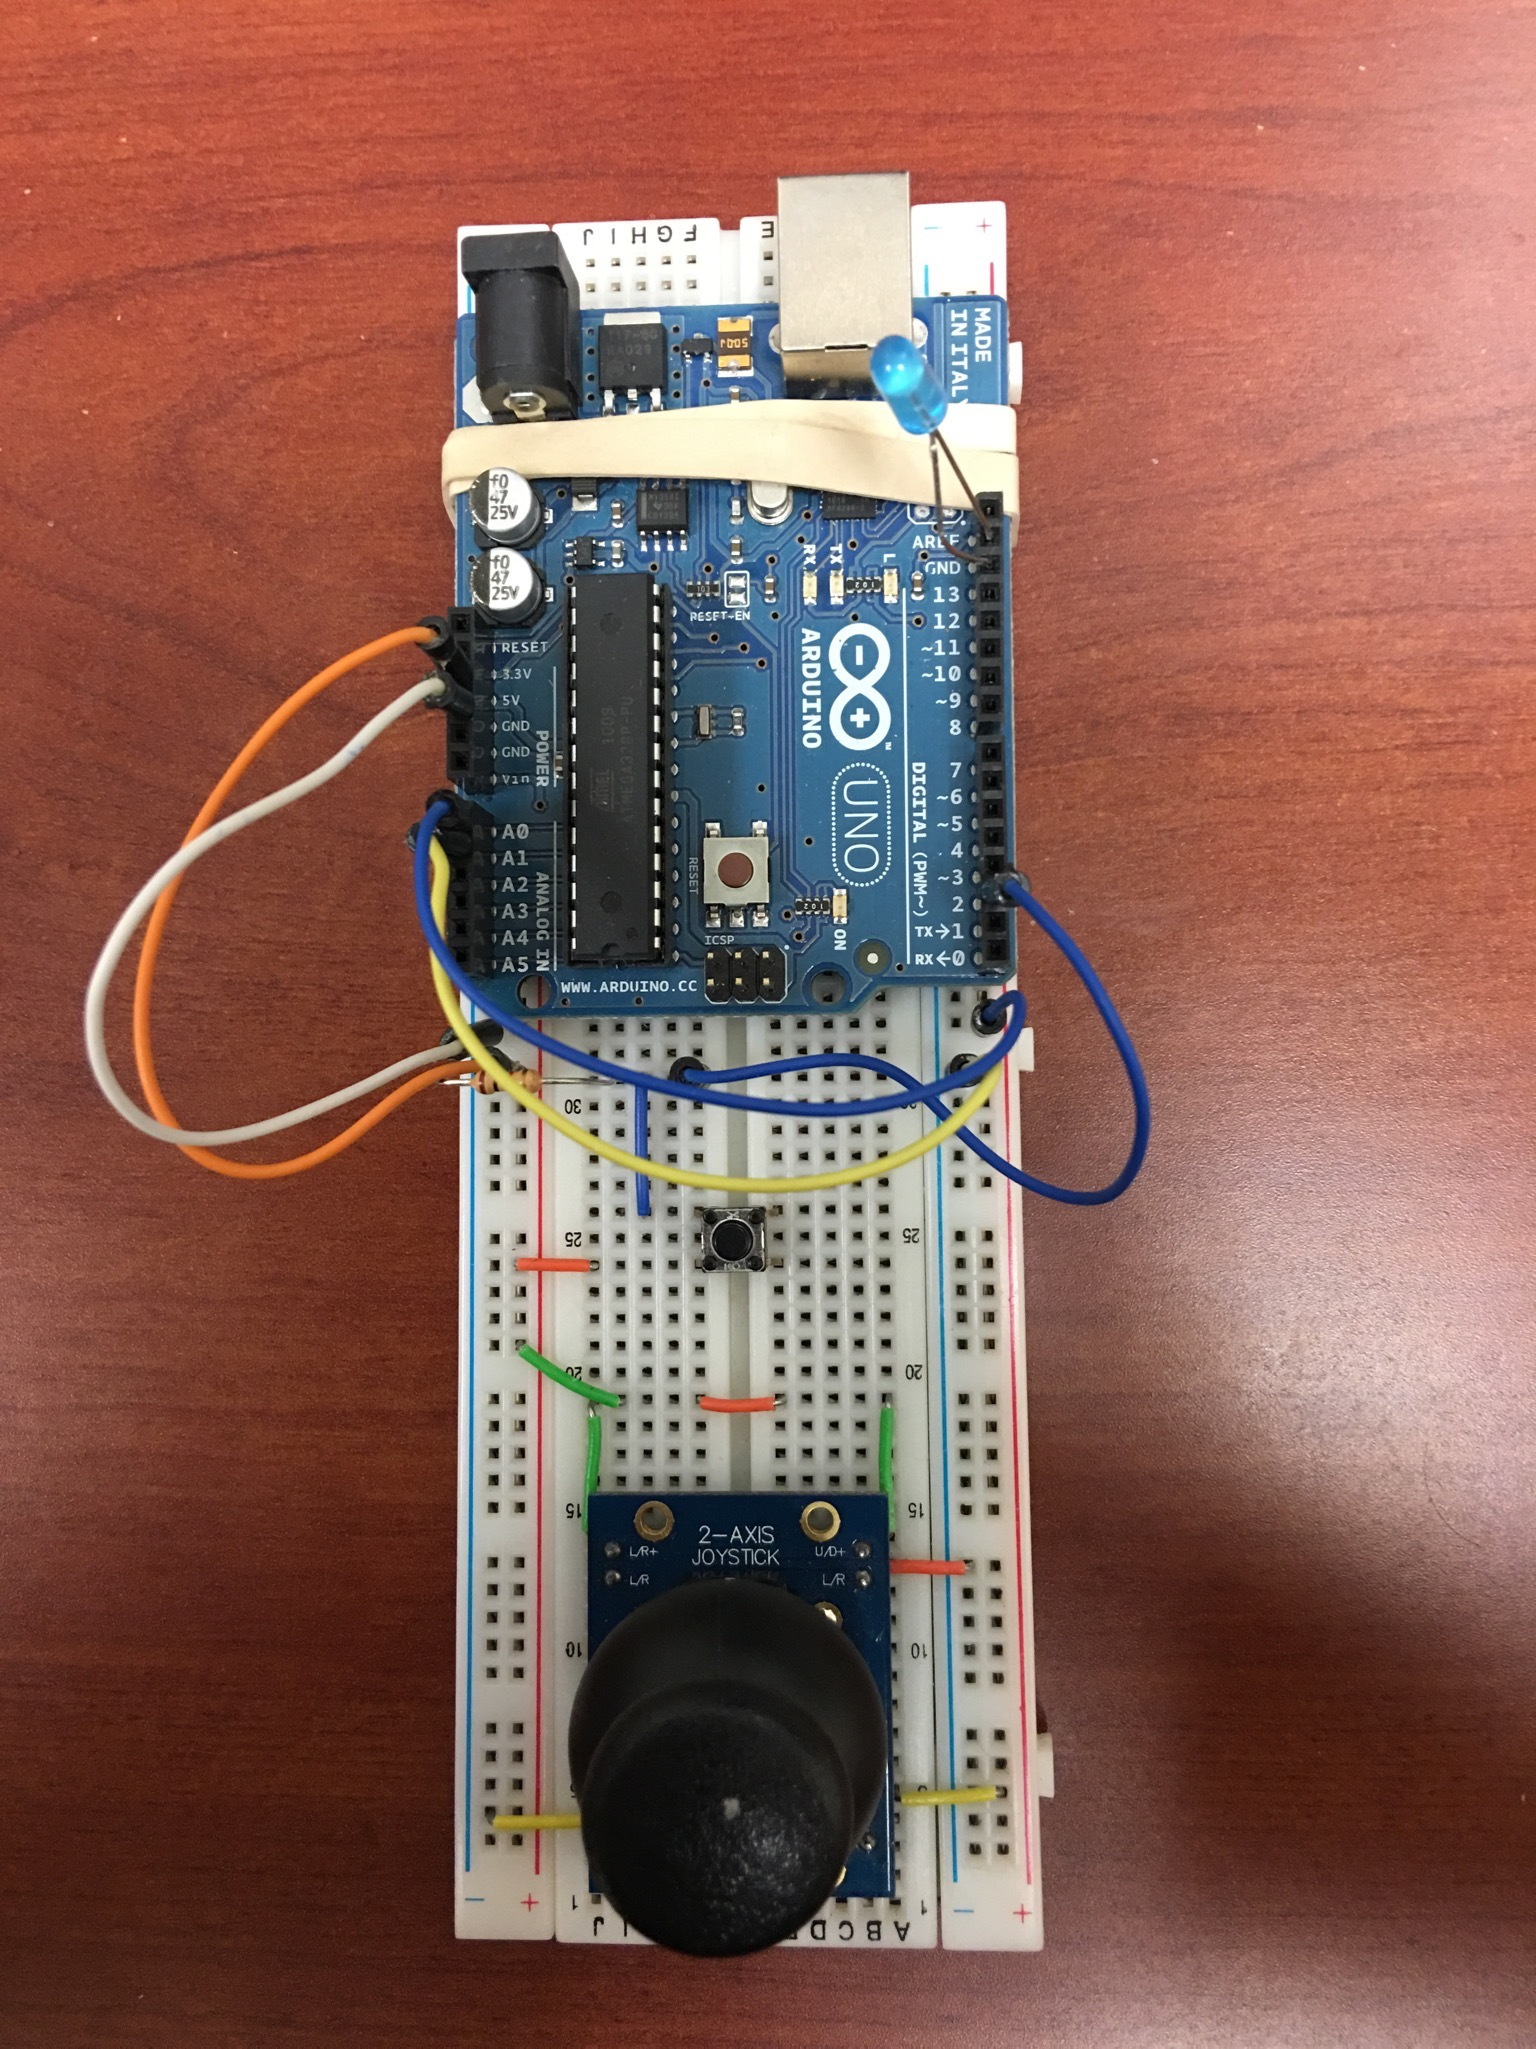
\includegraphics[scale=0.1]{arduino-gamecontroller/project}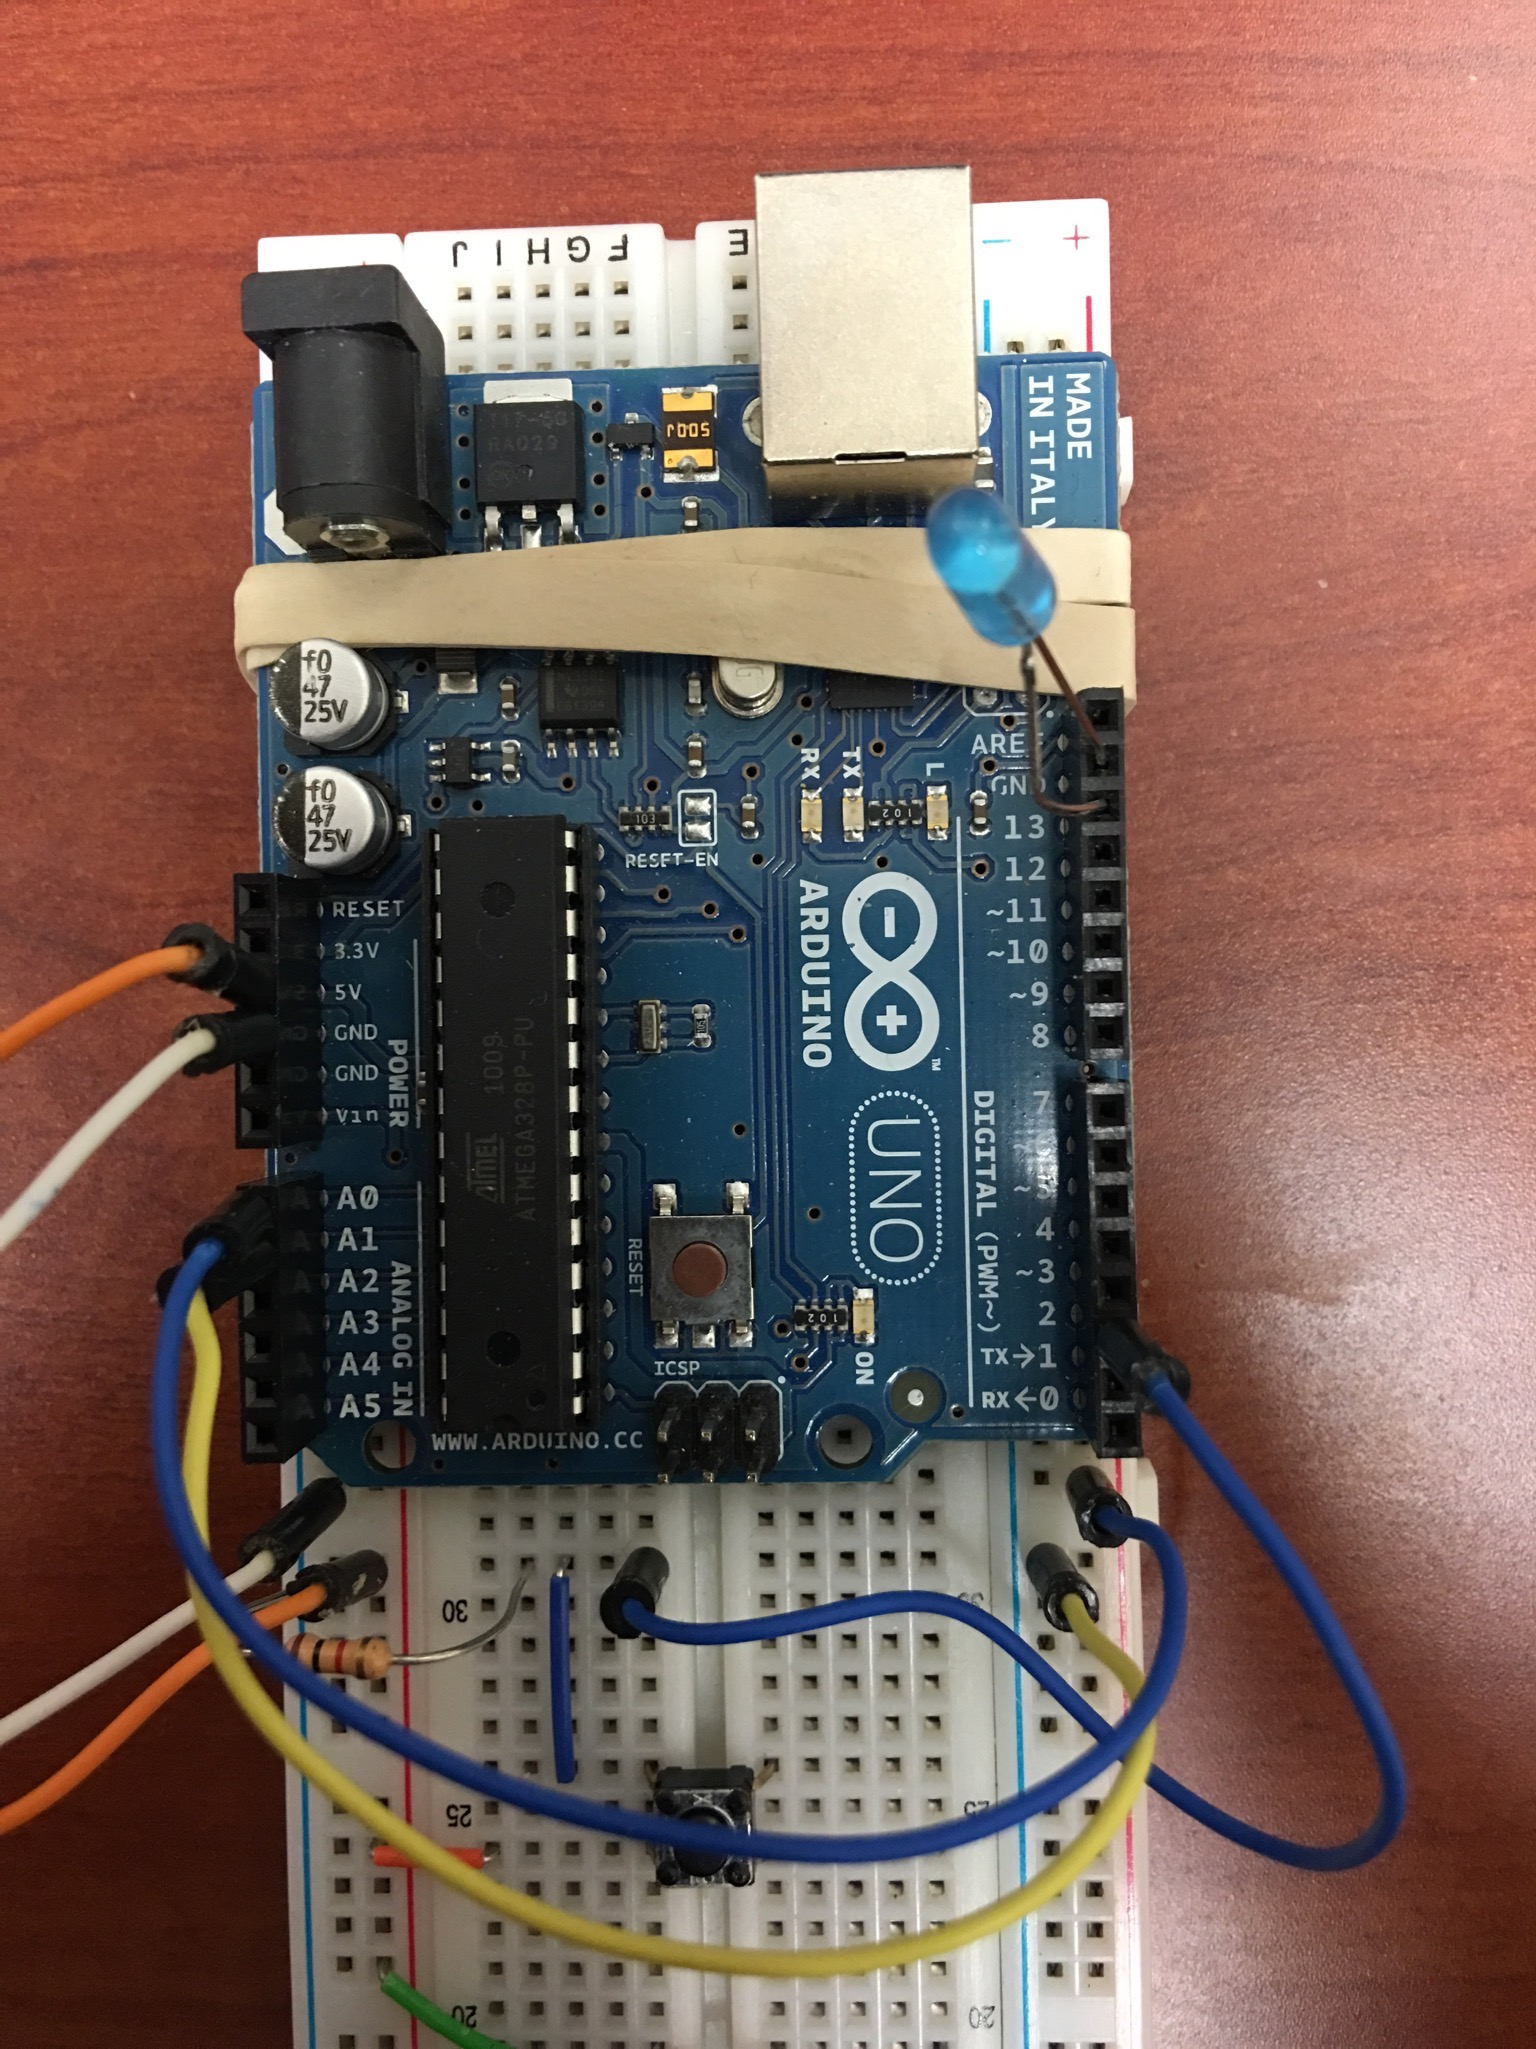
\includegraphics[scale=0.1]{arduino-gamecontroller/project-top}\\
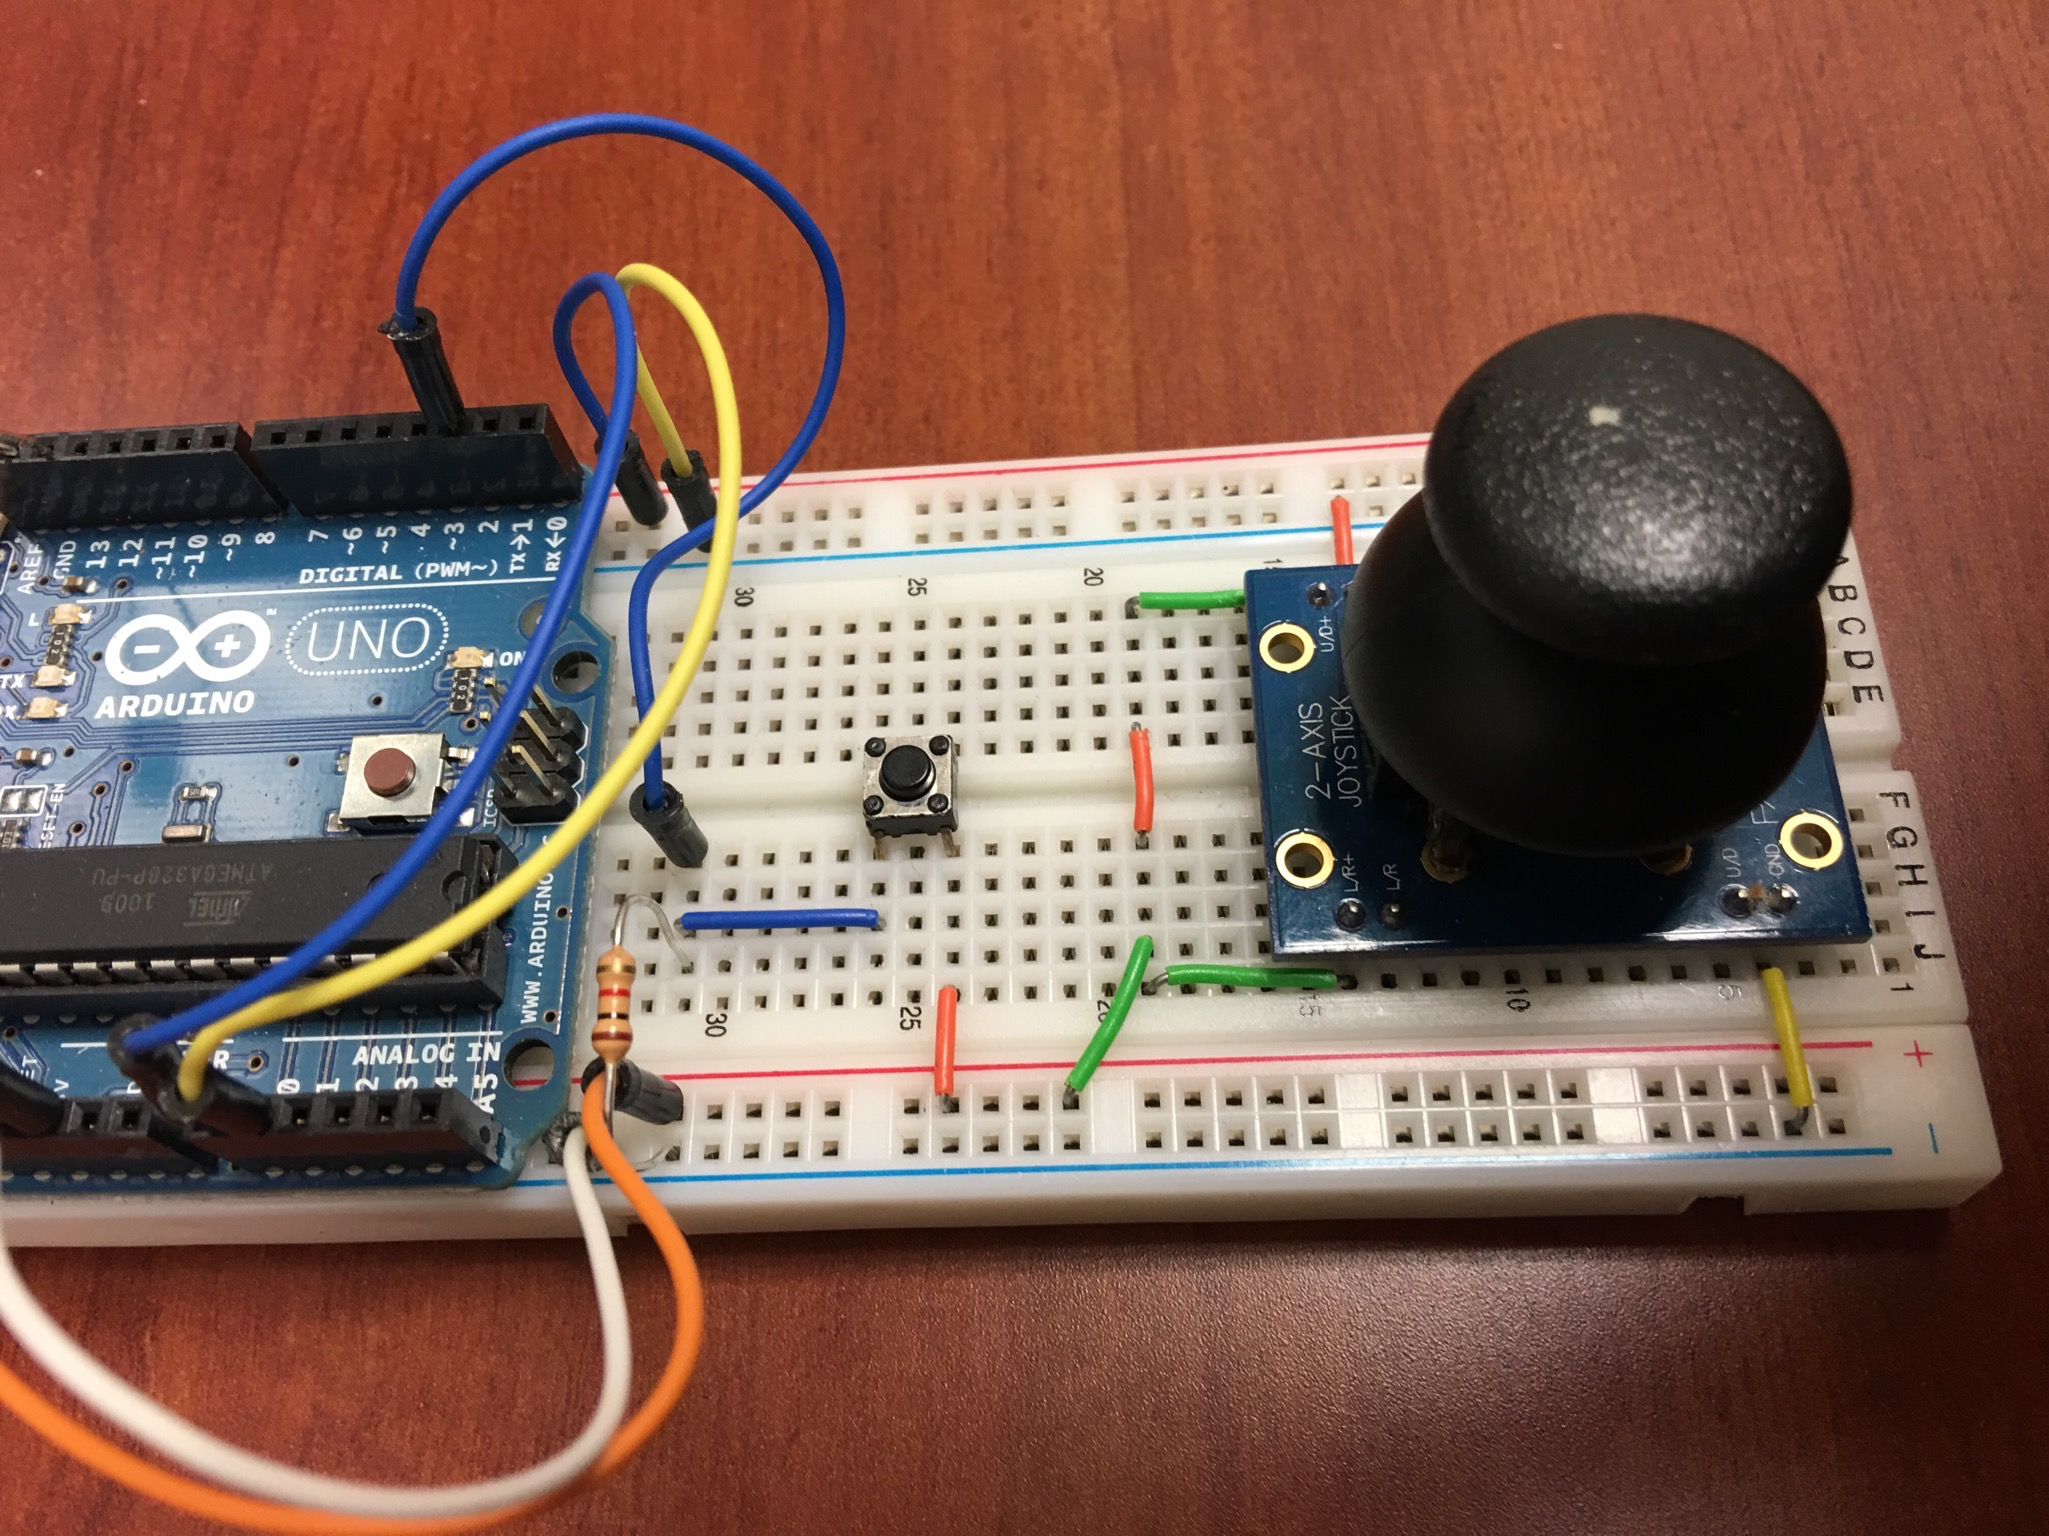
\includegraphics[scale=0.1]{arduino-gamecontroller/project-left}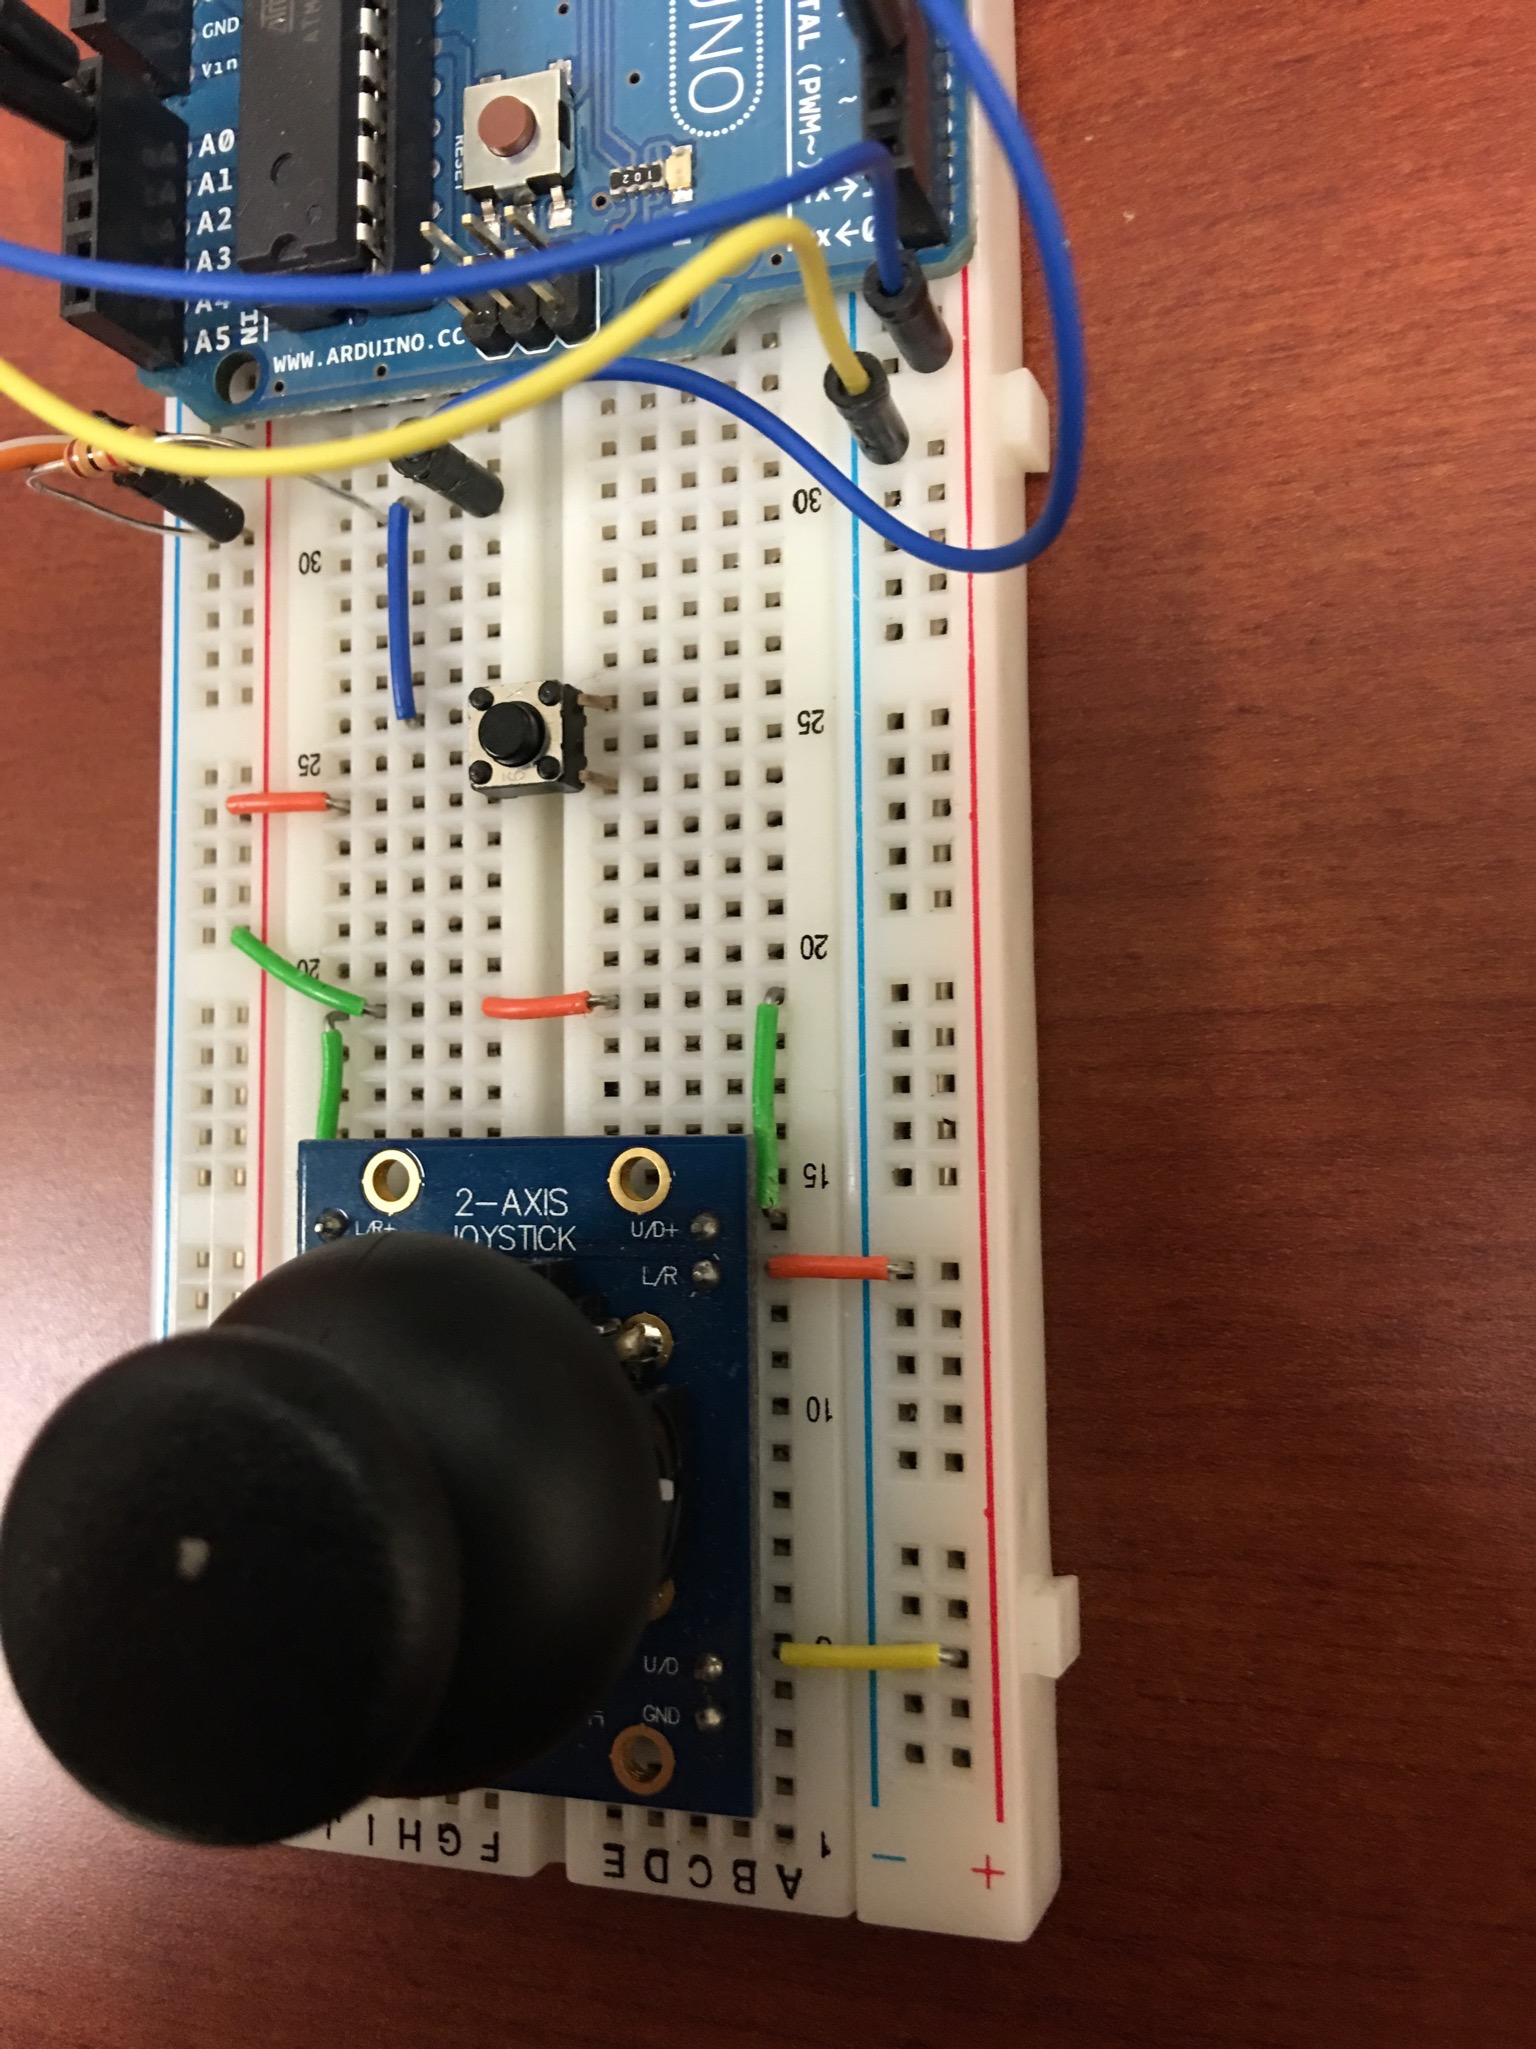
\includegraphics[scale=0.1]{arduino-gamecontroller/project-right}


\item Attach the Arduino to the breadboard with the rubber band.

\item Place the LED in pins 13 and GND. The LED has a long lead and a short lead. The long lead goes in pin 13 and the short lead goes in GND.

\item Run wires from GND (white wire) and +5 V (orange wire) pins on the left side of the Arduino to the -- and + columns on the left side of the breadboard, respectively. GND is wired to the -- column and 5 V is wired to the + column.

\item Run wires from pins A0 and A1 on the left side of the Arduino to the + and -- columns on the right side of the breadboard, respectively. A0 is wired to the +column an dA1 is wired to the -- column.

\item Attach the joystick to the breadboard. 

\item Wire the L/R+ and U/D+ pins on the joystick to +5 V (the + column on the left side of the breadboard).

\item Wire the GND pin on the joystick to GND (the -- column on the left side of the breadboard).

\item Wire the U/D pin on the joystick to pin A0 of the Arduino (the + column on the right side of the breadboard).

\item Wire the L/R pin on the joystick to pin A1 of the Arduino (the -- column on the right side of the breadboard).

\item The pushbutton switch, resistor, and the wire from pin 3 of the Arduino are not needed for the Lunar Lander game. You can add those parts later if you wish to fire bullets in Asteroids, for example.

\subsection*{Upload an Arduino program to the Arduino Uno}

We must upload a program to the Arduino that reads the voltage across each axis of the joystick and passed it to VPython when requested.

\item Download lunarLander.zip from our course web site. Here is the code.

\begin{arduinoblock}
#define UD A0
#define LR A1
int received;
char buffer[10];		  // input buffer
int N;			          // how many measurements to make
boolean done = false;


void setup() {
  Serial.begin(9600);
}

void loop() {
        received = 0;
    	buffer[received] = '\0';
    	done = false;
    
    	// Check input on serial line.
    	while (!done) {
    		if (Serial.available()) {	// Something is in the buffer
    			N = Serial.read();	// so get the number byte
    			done = true;
    		}
    	}
  
      int LRval = analogRead(LR);
      int UDval = analogRead(UD);
      Serial.print(LRval, DEC);
      Serial.print('\t');
      Serial.print(UDval, DEC);
      Serial.print('\n');
      delay(10);
}
\end{arduinoblock}

\item Open \code{lunarLander.ino}  with the Arduino software. The program looks like Figure \ref{arduino-gamecontroller/arduino-program}.

\scaledimage{arduino-gamecontroller/arduino-program}{An Arduino program running on the microprocessor.}{0.3}

\item Go to the \menu{Tools} menu and select \menu{Port}. One of these ports corresponds to the Arduino. Make sure  the correct one is checked, as shown in Figure \ref{arduino-gamecontroller/arduino-port}. This usually occurs by default.

\scaledimage{arduino-gamecontroller/arduino-port}{Select the serial port for your Arduiono}{0.3}

There are two important buttons in the top left corner of the menu bar. One is a checkmark and one is a right arrow, as shown in Figure \ref{arduino-gamecontroller/arduino-buttons}.

\scaledimage{arduino-gamecontroller/arduino-buttons}{Select the serial port for your Arduiono}{0.3}

\item The checkmark button is used to compile the Arduino program. It will tell you if there are any programming errors. Click the checkmark button to compile.

\item If there are no errors, then you are ready to upload the program to the microprocessor. Click the right arrow button to upload the program to the mircoprocessor.

The program should now be running on the microprocessor. It runs continuously in an infinite loop as long as it has power.

\subsection*{Running Lunar Lander with the Arduino game controller}

\item I have already created a Jupyter notebook that you can use as a template. Download the file \code{lunar-lander-nb.ipynb} from our course web site. Save the file (or move the file) into the folder where you stored your first Jupyter notebook file that you used to test the software.

\item  Go to the Jupyter browser window that shows your files and folders. Click on the file you just downloaded. It should open as a VPython notebook (as indicated in the top, right corner). 

\item Run the first cell. (It imports packages.)

\item The second cell has the code necessary to communicate with the Arduino. You need to get the serial port for your Arduino. Go to the Arduino software, click the \menu{Tools} menu and select \menu{Port}. Right down the name of the serial port that your Arduino is connected to. In your VPython notebook, edit the \code{port} variable to match the name of the port used by your Arduino. Mine is:

\begin{myvpython}
#serial port for the Arduino; get the name for the port from the Arduino software
port = '/dev/cu.usbmodem1a1221'
\end{myvpython}

Make sure the name of the port is contained within quotes since it is a string.

\item Run this cell and verify that there are no errors.

\item Run the third cell that contains the code for the game. You should see the lander, and you should be able to control it with your game controller.

%\scaledimage{arduino-gamecontroller/arduino-uno}{Arduino Uno microprocessor and breakout board.}{0.3}

\end{enumerate}

\pagebreak

\analysis

\begin{description}

\item[B] Complete this exercise and do the following.

\begin{enumerate}
	\item Upload a working notebook file produced at the end of this activity.
\end{enumerate}


\item[A] Do everything for {\bf B} with the following modifications and additions.

\begin{enumerate}
	\item Write a new game that uses the game controller and runs in a notebook.
\end{enumerate}




\end{description}




%Appendices
% Turn off lab numbering
\formatappendixtoc
%
%\myappendix{labnotebook}{Lab Notebook}

\bigskip
\noindent
The instructional laboratory serves various educational purposes which include

\begin{enumerate}
	\item training you to be a practicing scientist.
	\item training you to properly record your experiments in a lab notebook.
	\item covering essential topics such as proper use of equipment, safety, uncertainty in measurements and calculations, and graphical analysis.
	\item providing you with hands-on exercises that help you build conceptual models.
	\item challenging you with open-ended projects where you combine your knowledge and creativity to design an experiment or solve a problem.
	\item giving you additional opportunities to practice applying what you learn in the course.
\end{enumerate}

Your lab notebook should be:

\begin{enumerate}
	\item readable---A person should be able to pick up your lab notebook and completely reproduce the experiment. This requires proper detail, description, and organization. A picture is worth a thousand words, so use sketches regularly! But you don't have to follow proper grammar. (WHAT? That's heresy!) The lab notebook is not like a formal lab report or a journal article. It's a permanent, indisputable record of what you did in the laboratory. As long as your record is unambiguous to the point that someone else can reproduce the experiment, then it's clear enough. However, spelling is important because people hate reading misspelled words and because mispeling werds is imbarasing.
	\item complete---The lab notebook must contain the parts listed below for each experiment and follow proper rules for a lab notebook.
	\item accurate and precise---Experiments should be done with great care. ``\emph{Human error}" is not an acceptable excuse and is NOT the same as ``\emph{experimental error}." If there is human error, then redo the experiment. The quality of an experiment can be judged based on \emph{accuracy} and \emph{precision}.
\end{enumerate}

\subsection*{Elements of recording an experiment}

Each experiment in your lab notebook should have the following elements (taken from Dr. Bowman's guidelines used in CHM 299):

\begin{description}
	\item[Experiment or project number and date] The experiment, project number, or other method of identifying the experiment or test should be recorded here.
	\item[Title] A short descriptive title is very desirable.
	\item[Purpose] The purpose should indicate clearly the reason(s) for the experiment or the test.
	\item[Materials and source] It is important to properly identify the materials being used by part, Vendor (if possible), and any other appropriate description.
	\item[Procedure] Enter the exact procedure as completely and concisely as possible. Remember that enough detail should be included to permit someone else to carry out the experiment and obtain, essentially the same results.  Be as accurate and as quantitative as possible. Include all measurements with clear descriptions of those measurements. If data is stored electronically, then place the data file in an appropriate place on the computer with a descriptive name, and reference the path to the file in your lab notebook. You can even burn the file on a CD and include it with the lab notebook.  Do not hurry!  Take time to do this section right.  Your job may depend on it.
	\item[Drawing] If at all feasible, a well-labeled sketch or drawing (not necessarily to scale) should be prepared showing the equipment or arrangement of equipment used, particularly if special equipment or arrangements are involved.
	\item[Results obtained] Results include your own observations, test results, analyses, etc.  List the results obtained in a form that can be easily understood, e. g., tables, graphs, etc.  Give the details of any tests that were utilized to obtain the reported results. Printouts of graphs should be taped into the lab notebook, and the page number should be referenced. Electronic files of data, graphs, and/or analyses should be saved and referenced.
	\item[Conclusion or summary] Enter a short discussion of the significant results. The elements of invention are novelty, utility and unobviousness. State what you believe to be important about this result and what situations it might apply to. State the general idea to which the results allude.

Record the name of the person or persons who saw you carry out this work or to whom the results were described.  In this connection, it is entirely appropriate and even desirable, to call someone into your laboratory to see the experimental results, and if feasible, to repeat the experiment for someone's benefit in order to demonstrate the new result or product.

\item[Signature and date]

The record should be signed and dated immediately upon completion and no further additions' entered thereafter. Do not back date any record.

\item[Witness and date]

Remember that the witness must be able to testify that he or she read and understood the record in question on the day he or she signed as a witness. Therefore, the witness may be anyone who is able to understand what is written.  Usually this is someone in your research group.

The effective date of the record as it stands is the date of, corroboration, i.e.  the day it is witnessed. Ask someone to read and witness your record as soon as it is completed, but do not ask or allow the witness to backdate his or her signature.  Clearly, to obtain the earliest effective date, it is best to have the witness review your work often.  It is also courteous to reciprocate by reviewing the work of the witness.
\end{description}

\subsection*{Rules for keeping a lab notebook}

\begin{enumerate}
	\item Write in permanent ink.
	\item If you make a mistake, strike through the error once and initial.
	\item Include a table of contents at the beginning of the notebook. After adding a new experiment to your notebook, add an entry to the table of contents page that references the experiment.
	\item Leave no blank space in the notebook. If you wish to start at the top of the next page, then draw a line through the remaining blank space on the previous page.
	\item Use a Table of Contents at the beginning of the lab notebook and enter experiment names and the starting page numbers for those experiments. One should be able to open to the table of contents and see a list of experiments performed and recorded in the lab notebook.
\end{enumerate}

%\myappendix{functionsandgraphs}{Functions and Graphs}

When making a graph, you generally plot the independent variable on the x-axis and the dependent variable on the y-axis as shown in Figure \ref{appendix-functions-and-graphs/y-x}.  Since $y$ depends on x, then we can determine the functional relationship, $y=f(x)$ by analyzing the graph.

\scaledimage{appendix-functions-and-graphs/y-x}{Dependent variable on the $y$ axis and independent variable on the $x$ axis.}{0.8}

There are many relationships between $y$ and $x$ that are common in physics.  Here are a few typical ones.

\subsection*{y is directly proportional to x}

This relationship is described by the equation

\begin{eqnarray*}
	y & = & mx \\
\end{eqnarray*}

where $m$ is the slope of the graph. The result is a straight line of non-zero slope that passes through the origin, so that $y=$ at $x=0$, as shown in Figure \ref{appendix-functions-and-graphs/direct}.

\scaledimage{appendix-functions-and-graphs/direct}{$y$ is directly proportional to $x$}{0.8}

\subsection*{y is linearly related to x}

This relationship is described by the equation

\begin{eqnarray*}
	 y & = &  mx+b
\end{eqnarray*}	 

where $m$ is the slope and $b$ is the y-intercept.  The resulting graph is a line of constant, non-zero slope.  Note that the slope is not necessarily positive and the y-intercept is not necessarily zero.  In the graph in Figure \ref{appendix-functions-and-graphs/linear}, the slope is negative and the y-intercept is equal to 3.

\scaledimage{appendix-functions-and-graphs/linear}{y is linearly related to x.}{0.8}
 
\subsection*{y is proportional to the square root of x}

When $y^2$ is proportional to x, the graph is a side-opening parabola.  The equation that describes this relationship is

\begin{eqnarray*}
	 y^2 & = & Cx
\end{eqnarray*}	 
 
and the graph looks something like the one shown in Figure \ref{appendix-functions-and-graphs/y2-x}. Taking the square root of Eq. 3  and setting the constant $\sqrt{C}$ to the letter $A$ shows that $y$ is proportional to $\sqrt{x}$.

\begin{eqnarray*}
	 y& = & A\sqrt{x}
\end{eqnarray*}	

\scaledimage{appendix-functions-and-graphs/y2-x}{$y$ is proportional to $\sqrt{x}$}{0.8}


\subsection*{quadratic}

This relationship is a top-opening parabola like graph shown in Figure \ref{appendix-functions-and-graphs/y-x2}.


\scaledimage{appendix-functions-and-graphs/y-x2}{quadratic}{0.8}

 
The equation that describes this relationship is

\begin{eqnarray*}
	 y & = &  ax^2+bx+c
\end{eqnarray*}	 

The constant $a$ determines the value of $y$ at $x =0$. The constant $b$ determines the slope of a tangent line (i.e. line tangent to the function) at $x=0$. The constant $c$ determines the concavity of the parabola.  If $c$ is positive, the function has an upward concavity. If $c$ is negative, then the function has a downward concavity.  Can you figure out what the signs are for the constants $a$, $b$, and $c$ in the previous graph?

\subsection*{$y$ is inversely proportional to x}

For this relationship, as $x$ gets larger, $y$ gets smaller.  As $x$ gets smaller, $y$ gets larger.  The equation relating $y$ and $x$ is of the form:

\begin{eqnarray*}
	 y & = &  \frac{A}{x}
\end{eqnarray*}	 

This curve assymptically approaches $y=0$ as $x\to\infty$.  Also, notice that as $x$ approaches zero, $y$ becomes infinite. An example graph of $y$ vs. $x$ for an inverse relationship is shown in Figure \ref{appendix-functions-and-graphs/inverse}.

\scaledimage{appendix-functions-and-graphs/inverse}{$y$ is inversely proportional to $x$}{0.8}

\newpage

\subsection*{$y$ is proportional to the cosine (or sine) of x}

For this relationship, $y$ ``oscillates."  The equation relating $y$ and $x$ is

\begin{eqnarray*}
	 y & = &  Acos(\omega x + \phi) + C
\end{eqnarray*}	 

This relationship is referred to as \emph{sinusoidal} regardless of whether you choose to use the cosine or sine function. The constant, $A$, is called the amplitude.  $\omega$ is called the angular frequency. $\phi$ is called the phase.  Whether the equation is written with a cosine function or with a sine function is unimportant. It simply alters the value of the phase. The constant, $C$, shifts the entire function upward or downward on the graph.

An example graph of $y$ vs. $x$ for a sinusoidal relationship is shown in Figure \ref{appendix-functions-and-graphs/sine}.

\scaledimage{appendix-functions-and-graphs/sine}{$y$ is sinusoidal}{0.8}


\subsection*{No relationship between $y$ and $x$}

If there is no relationship between $y$ and x, then changing $x$ will not result in a change in $y$.  In other words, $y$ is constant, regardless of the value of $x$.  What does a graph look like if $y$ is constant?  It is a straight line of zero slope as shown in Figure \ref{appendix-functions-and-graphs/no-relationship}.


\scaledimage{appendix-functions-and-graphs/no-relationship}{$y$ is not related to $x$}{0.8}


\myappendix{tracker}{Tracker Cheat Sheet}

\subsection*{Description}

This one-page ``cheat sheet'' will show you the most common steps required to analyze videos with Tracker.Tracker is developed by Doug Brown and is available from \url{http://www.cabrillo.edu/~dbrown/tracker/}.

\subsection*{Preliminary Steps}

\begin{enumerate}
	\item Go to \menu{Video$\to$Import\dots} and select the video you wish to analyze.
	
	\scaledimage{./appendix-tracker/import}{Import your video.}{0.3}
	
	\item Click the movie settings icon 
\includegraphics[scale=0.8]{./appendix-tracker/movie-settings} and set the frame rate, start frame, and end frame. Note that setting the start frame and end frame is quite useful for trimming the movie to just the part that is of interest.
	
	\item Click the calibration icon 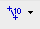
\includegraphics[scale=0.7]{./appendix-tracker/calibration} and select one of the calibration tools. Stretch the tool across an object of known length, such as a meterstick, that is in the plane of the motion. Click on the numeric indicator for the length of the tool and change the value to be the length of your standard object in the video.
	
	\item Click the coordinate system icon 
\includegraphics[scale=0.7]{./appendix-tracker/coord-sys} and move the origin of the coordinate system to the desired location. Grab the x-axis and rotate it in order to set the direction of the coordinate system. 	
	
\end{enumerate}

\subsection*{Mark an object}

\begin{enumerate}
	\item Click the \button{Create} button and select \menu{Point Mass}.
	\item In the toolbar, a menu for \menu{mass A} will appear.  
\includegraphics[scale=0.5]{./appendix-tracker/massA} Click on \menu{mass A} in order to select its \menu{Name\dots}, \menu{Color\dots}, or other parameters.
	\item {\bf \emph{While holding the shift key}}, click on the object. A mark will appear, and the video will advance to the next frame.
\end{enumerate}

\subsection*{Analyze a graph}

\begin{enumerate}
	\item Right-click on the graph and select \menu{Analyze\dots}. The Data Tool window will pop up. 
	\item Check \button{\ding{51}}Fit, and the Fit menus and parameters will appear. 
	\item Check \button{\ding{51}}Autofit for the Data Tool to automatically calculate the best-fit parameters.
	\item To fit a curve to a portion of the data, select the data in the graph or data table.
\end{enumerate}


\myappendix{project1}{Project 1 -- Developing your first game with constant velocity motion}

\longgoal

For this project, you will develop a game using objects that move with constant velocity. The result will count toward your Quiz 1 grade.

\section*{Project Guidelines}

You will develop a game that involves objects that move with constant velocity. It is due at 3 PM in Feb. 9. Upload your game via Moodle. On Thursday, Feb 2 and Tuesday, Feb. 7, you can get help with your program. You can also get help from Zach Shore on Monday and Wednesday in Rm 102 from 4:15 PM -- 5:15 PM.\\

\noindent
There are four categories that the project's grade is based on.

\begin{enumerate}
	\item level of difficulty (i.e. "Is the game more interesting than just a ball bouncing back and forth on the screen?" and "Is it sufficiently different from the one developed in class?" and "Is the game fun to play?").  Note that you should be creative, but don't try writing a game that exceeds your abilities at this point. My criteria for projects are to choose something that is (1) doable and (2) interesting.
	\item level of independence.  Using resources is good, but you can't copy another program or have someone else write the code for you. Always cite your references, including people who help you.
	\item completeness (i.e.  "Does the simulation run?" or  or "Did the program include objects that move with constant velocity?" or "Does the program work as expected?")
	\item quality of documentation ("Did you include relevant references?" or "Did others test your game?")
\end{enumerate}

\noindent
You should:

\begin{enumerate}
	\item write a VPython program that includes objects that move with constant velocity.
	\item test your game by having others play it and by asking them for feedback.
	\item answer the questions below in a Word document.
\end{enumerate}

\section*{Documentation}

You must write a document in Word that answers the following questions. The document should be complete; it should have correct grammar; and it should be easy to read and understand. Quality writing and organization is expected.

\begin{enumerate}
	\item What is the purpose of your game?
	\item What are the rules of your game?
	\item How must the game be played (i.e. keystrokes, etc.)?
	\item Is this game like any other game that you've seen or played?
	\item Who played your game and what did you learn as a result of their feedback?
	\item What resources did you use to help you in writing the game?  If you used web sites, people (such as Dr. T or the S.I.), books, or any other resources, you must reference them.
	\item What did you personally get out of this project?
\end{enumerate}


\myappendix{project-final}{Final Project -- Developing an Original Game}

\longgoal

For this project, you will develop an original game that incorporates moving objects that obey the laws of physics. This includes objects that move with constant velocity or constant acceleration, objects with correct relative motion (such as bullets shot from a moving shooter), projectiles, and objects that explode into pieces (like in the game Asteroids).

\section*{Project Guidelines}

You will develop a game that involves moving objects that obey the laws of physics. It is due on at the beginning of our Final Exam time.\\

\noindent
There are six categories that the project's grade is based on.

\begin{enumerate}
	\item level of difficulty (``How does your game compare to the ones written for this class in terms of difficulty?'' or ``Is the code written for your project similar to A-level exercises in our class in terms of difficulty?'' or ``Does your game include competitive aspects?'')
	\item level of creativity (``Is this game exactly like ones we've done in class or have you reached to do something innovative?'' or ``Did you try to duplicate other popular games?'' or ``Did you add correct physics to a popular game that did not have correct physics?'')
	\item level of independence.  Using resources is good, but you can't copy another program or having someone else write the code for you. Always cite your references, including people who help you. Be sure to cite the page numbers from our class handouts that were used for your project. 
	\item completeness (i.e.  "Does the simulation run?" or  or "Did the program include objects that move with constant velocity?" or "Does the program work as expected?")
	\item quality of documentation ("Did you include relevant references?" or "Did others test your game?")
	\item quality of your presentation (``Did you discuss the purpose of the game?'' or ``Did you discuss the rules of the game?'' or ``Did you discuss the physics principles used in the game?'')
\end{enumerate}

\noindent
You should:

\begin{enumerate}
	\item write a VPython program that includes objects that move.
	\item test your game by having others play it and by asking them for feedback.
	\item answer the questions below in a Word document.
	\item create and deliver a presentation about the game.
\end{enumerate}

\section*{Documentation}

You must write a document in Microsoft Word or pdf format that answers the following questions. The document should be complete; it should have correct grammar; and it should be easy to read and understand. Quality writing and organization is expected. Detail is required. Terse responses will not receive significant credit. 

\begin{enumerate}
	\item What is the purpose of your game?
	\item What are the rules of your game?
	\item How must the game be played (i.e. keystrokes, etc.)?
	\item Is this game like any other game that you've seen or played?
	\item What physics principles were used in your game in order to make it realistic?  Be sure to cite the physics principle(s) (such as projectile motion, constant velocity motion, constant acceleration motion, relative motion, center of mass motion, etc.) and where these principles were discussed in our course handouts. Be sure to reference the page number(s).
	\item Does your game violate any laws of physics? (Note that sometimes this is desirable for playability or artistry.)
	\item Who played your game and what did you learn as a result of their feedback?
	\item How might you improve your game in the future?
	\item What resources did you use to help you in writing the game?  If you used web sites, people (such as Dr. T or Zach), books, or any other resources, you must reference them.
	\item What did you personally get out of this project?
\end{enumerate}

\section*{Presentation}

You will give a seven minute presentation. Five minutes will be for the presentation and two minutes will be for questions. You are expected to create a Keynote, Powerpoint, or pdf document that:

\begin{enumerate}
	\item describes the purpose of the game.
	\item describes the rules of the game.
	\item describes how the game is played.
	\item describes which physics principles were used in the game.
	\item how the game can be improved.
\end{enumerate}

You are also expected to demonstrate your game by playing the game.

Your presentation will be graded on:

\begin{enumerate}
	\item whether others acted interested in your game by giving feedback or asking questions.
	\item whether you spoke clearly and were organized in your presentation.
	\item whether you addressed the items above in your presentation.
	\item whether you demonstrated relative aspects of your game.
	\item whether you were enthusiastic about your game.
\end{enumerate}



\end{document}